% Options for packages loaded elsewhere
\PassOptionsToPackage{unicode}{hyperref}
\PassOptionsToPackage{hyphens}{url}
%
\documentclass[
]{book}
\usepackage{lmodern}
\usepackage{amsmath}
\usepackage{ifxetex,ifluatex}
\ifnum 0\ifxetex 1\fi\ifluatex 1\fi=0 % if pdftex
  \usepackage[T1]{fontenc}
  \usepackage[utf8]{inputenc}
  \usepackage{textcomp} % provide euro and other symbols
  \usepackage{amssymb}
\else % if luatex or xetex
  \usepackage{unicode-math}
  \defaultfontfeatures{Scale=MatchLowercase}
  \defaultfontfeatures[\rmfamily]{Ligatures=TeX,Scale=1}
\fi
% Use upquote if available, for straight quotes in verbatim environments
\IfFileExists{upquote.sty}{\usepackage{upquote}}{}
\IfFileExists{microtype.sty}{% use microtype if available
  \usepackage[]{microtype}
  \UseMicrotypeSet[protrusion]{basicmath} % disable protrusion for tt fonts
}{}
\makeatletter
\@ifundefined{KOMAClassName}{% if non-KOMA class
  \IfFileExists{parskip.sty}{%
    \usepackage{parskip}
  }{% else
    \setlength{\parindent}{0pt}
    \setlength{\parskip}{6pt plus 2pt minus 1pt}}
}{% if KOMA class
  \KOMAoptions{parskip=half}}
\makeatother
\usepackage{xcolor}
\IfFileExists{xurl.sty}{\usepackage{xurl}}{} % add URL line breaks if available
\IfFileExists{bookmark.sty}{\usepackage{bookmark}}{\usepackage{hyperref}}
\hypersetup{
  pdftitle={ImpactTB/BAA: Standard Operating Procedures for Data Analysis},
  pdfauthor={Colorado State University Coding Team},
  hidelinks,
  pdfcreator={LaTeX via pandoc}}
\urlstyle{same} % disable monospaced font for URLs
\usepackage{color}
\usepackage{fancyvrb}
\newcommand{\VerbBar}{|}
\newcommand{\VERB}{\Verb[commandchars=\\\{\}]}
\DefineVerbatimEnvironment{Highlighting}{Verbatim}{commandchars=\\\{\}}
% Add ',fontsize=\small' for more characters per line
\usepackage{framed}
\definecolor{shadecolor}{RGB}{248,248,248}
\newenvironment{Shaded}{\begin{snugshade}}{\end{snugshade}}
\newcommand{\AlertTok}[1]{\textcolor[rgb]{0.94,0.16,0.16}{#1}}
\newcommand{\AnnotationTok}[1]{\textcolor[rgb]{0.56,0.35,0.01}{\textbf{\textit{#1}}}}
\newcommand{\AttributeTok}[1]{\textcolor[rgb]{0.77,0.63,0.00}{#1}}
\newcommand{\BaseNTok}[1]{\textcolor[rgb]{0.00,0.00,0.81}{#1}}
\newcommand{\BuiltInTok}[1]{#1}
\newcommand{\CharTok}[1]{\textcolor[rgb]{0.31,0.60,0.02}{#1}}
\newcommand{\CommentTok}[1]{\textcolor[rgb]{0.56,0.35,0.01}{\textit{#1}}}
\newcommand{\CommentVarTok}[1]{\textcolor[rgb]{0.56,0.35,0.01}{\textbf{\textit{#1}}}}
\newcommand{\ConstantTok}[1]{\textcolor[rgb]{0.00,0.00,0.00}{#1}}
\newcommand{\ControlFlowTok}[1]{\textcolor[rgb]{0.13,0.29,0.53}{\textbf{#1}}}
\newcommand{\DataTypeTok}[1]{\textcolor[rgb]{0.13,0.29,0.53}{#1}}
\newcommand{\DecValTok}[1]{\textcolor[rgb]{0.00,0.00,0.81}{#1}}
\newcommand{\DocumentationTok}[1]{\textcolor[rgb]{0.56,0.35,0.01}{\textbf{\textit{#1}}}}
\newcommand{\ErrorTok}[1]{\textcolor[rgb]{0.64,0.00,0.00}{\textbf{#1}}}
\newcommand{\ExtensionTok}[1]{#1}
\newcommand{\FloatTok}[1]{\textcolor[rgb]{0.00,0.00,0.81}{#1}}
\newcommand{\FunctionTok}[1]{\textcolor[rgb]{0.00,0.00,0.00}{#1}}
\newcommand{\ImportTok}[1]{#1}
\newcommand{\InformationTok}[1]{\textcolor[rgb]{0.56,0.35,0.01}{\textbf{\textit{#1}}}}
\newcommand{\KeywordTok}[1]{\textcolor[rgb]{0.13,0.29,0.53}{\textbf{#1}}}
\newcommand{\NormalTok}[1]{#1}
\newcommand{\OperatorTok}[1]{\textcolor[rgb]{0.81,0.36,0.00}{\textbf{#1}}}
\newcommand{\OtherTok}[1]{\textcolor[rgb]{0.56,0.35,0.01}{#1}}
\newcommand{\PreprocessorTok}[1]{\textcolor[rgb]{0.56,0.35,0.01}{\textit{#1}}}
\newcommand{\RegionMarkerTok}[1]{#1}
\newcommand{\SpecialCharTok}[1]{\textcolor[rgb]{0.00,0.00,0.00}{#1}}
\newcommand{\SpecialStringTok}[1]{\textcolor[rgb]{0.31,0.60,0.02}{#1}}
\newcommand{\StringTok}[1]{\textcolor[rgb]{0.31,0.60,0.02}{#1}}
\newcommand{\VariableTok}[1]{\textcolor[rgb]{0.00,0.00,0.00}{#1}}
\newcommand{\VerbatimStringTok}[1]{\textcolor[rgb]{0.31,0.60,0.02}{#1}}
\newcommand{\WarningTok}[1]{\textcolor[rgb]{0.56,0.35,0.01}{\textbf{\textit{#1}}}}
\usepackage{longtable,booktabs}
\usepackage{calc} % for calculating minipage widths
% Correct order of tables after \paragraph or \subparagraph
\usepackage{etoolbox}
\makeatletter
\patchcmd\longtable{\par}{\if@noskipsec\mbox{}\fi\par}{}{}
\makeatother
% Allow footnotes in longtable head/foot
\IfFileExists{footnotehyper.sty}{\usepackage{footnotehyper}}{\usepackage{footnote}}
\makesavenoteenv{longtable}
\usepackage{graphicx}
\makeatletter
\def\maxwidth{\ifdim\Gin@nat@width>\linewidth\linewidth\else\Gin@nat@width\fi}
\def\maxheight{\ifdim\Gin@nat@height>\textheight\textheight\else\Gin@nat@height\fi}
\makeatother
% Scale images if necessary, so that they will not overflow the page
% margins by default, and it is still possible to overwrite the defaults
% using explicit options in \includegraphics[width, height, ...]{}
\setkeys{Gin}{width=\maxwidth,height=\maxheight,keepaspectratio}
% Set default figure placement to htbp
\makeatletter
\def\fps@figure{htbp}
\makeatother
\setlength{\emergencystretch}{3em} % prevent overfull lines
\providecommand{\tightlist}{%
  \setlength{\itemsep}{0pt}\setlength{\parskip}{0pt}}
\setcounter{secnumdepth}{5}
\usepackage{booktabs}
\usepackage{amsthm}
\makeatletter
\def\thm@space@setup{%
  \thm@preskip=8pt plus 2pt minus 4pt
  \thm@postskip=\thm@preskip
}
\makeatother
\ifluatex
  \usepackage{selnolig}  % disable illegal ligatures
\fi
\usepackage[]{natbib}
\bibliographystyle{apalike}

\title{ImpactTB/BAA: Standard Operating Procedures for Data Analysis}
\author{Colorado State University Coding Team}
\date{2022-12-06}

\begin{document}
\maketitle

{
\setcounter{tocdepth}{1}
\tableofcontents
}
\hypertarget{overview}{%
\chapter{Overview}\label{overview}}

\hypertarget{about-the-project}{%
\section{About the project}\label{about-the-project}}

The objective of the Immune Mechanisms of Protection against Mycobacterium tuberculosis (IMPAc-TB) program is to get a thorough understanding of the immune responses necessary to avoid initial infection with \emph{Mycobacterium tuberculosis (Mtb)}, formation of latent infection, and progression to active TB illness. To achieve these goals, the National Institute of Allergy and Infectious Diseases awarded substantial funding and established multidisciplinary research teams that will analyze immune responses against \emph{Mtb} in animal models (mice, guinea pigs, and non-human primates) and humans, as well as immune responses elicited by promising vaccine candidates. The contract awards establish and give up to seven years of assistance for IMPAc-TB Centers to explain the immune responses required for \emph{Mtb} infection protection.

The seven centers that are part of the study are (in alphabetical order):

\begin{enumerate}
\def\labelenumi{\arabic{enumi}.}
\tightlist
\item
  Colorado State University
\item
  Harvard T.H. Chan School of Public Health
\item
  Seattle Children Hospital
\item
  {[}more{]}
\end{enumerate}

Colorado State University Team and role of each member:

\begin{itemize}
\tightlist
\item
  Dr.~Marcela Henao-Tamayo: Principal Investigator
\item
  Dr.~Brendan Podell: Principal Investigator
\item
  Dr.~Andres Obregon-Henao: Research Scientist-III
\item
  Dr.~Taru S. Dutt: Research Scientist-I
\item
  {[}more{]}
\end{itemize}

\hypertarget{about-this-book}{%
\section{About this book}\label{about-this-book}}

The aim of this book is to provide data protocols and data collection templates
for key types of data that are collected over the course of this project. By using
standard templates to record data, as well as starting from defined pipelines to
process and analyze the data, we aim to standardize the collection and processing
of data across this project.

Here, we have built a comprehensive guide to wet lab data collection, sample processing, and computational tool creation for robust and efficient data analysis and dissemination.

\hypertarget{experimental-metadata}{%
\chapter{Experimental metadata}\label{experimental-metadata}}

Metadata for an experiment:

\begin{itemize}
\tightlist
\item
  \texttt{species}
\item
  \texttt{start\_date}
\item
  \texttt{end\_date}
\item
  \texttt{experimental\_groups}
\end{itemize}

\hypertarget{animal-initial-conditions-and-weekly-weights}{%
\chapter{Animal initial conditions and weekly weights}\label{animal-initial-conditions-and-weekly-weights}}

\hypertarget{downloads}{%
\subsection{Downloads}\label{downloads}}

The downloads for this chapter are:

\begin{itemize}
\tightlist
\item
  \href{https://github.com/csu-impactb/CODING-TEAM-BOOKDOWN-/raw/main/templates/data_collection_templates/body_weights_template.xlsx}{Data collection template} for collecting initial information about the experimental animals and regular weight measurements, cage changes, and adverse events throughout the experiment
\item
  \href{https://raw.githubusercontent.com/csu-impactb/CODING-TEAM-BOOKDOWN-/main/templates/report_templates/animal_weights.Rmd}{Report template} to process data collected with the template (when you go to this link, go to the ``File'' bar in your browser's menu bar, chose ``Save As'', then save the file as ``animal\_weights.Rmd'')
\item
  \href{https://github.com/csu-impactb/CODING-TEAM-BOOKDOWN-/raw/main/templates/report_templates/animal_weights.docx}{Example output} from the report template
\end{itemize}

\hypertarget{overview-1}{%
\subsection{Overview}\label{overview-1}}

We use the template in this section to record information about each animal
used in the experiment. This includes the species, sex, and experimental group.
It also includes some information to identify the animal, which in the case
of mice includes a code describing the pattern of notches put in the mouse's
ear and the cage that the animal is assigned to at the beginning of the
experiment. These are all values that can be determined at the start of the
experiment, when the mice are first assigned to groups.

This template is also used to record some data over the course of the
experiment. This includes adverse events and cases where an animal is moved from
one cage to another during the experiment.

In addition, in our experiments, we are measuring the mice every week to record
their weight over the course of the experiment. This weight measuring begins
before the first vaccination and continues through until the last mouse is
sacrificed. We have used ear notches to identify each mouse, and between the ear
notch and the mouse's cage number, we can uniquely track each mouse in the
study.

There are a few reasons that we are measuring these mouse weights. The first is
to help us manage the mice, particularly in terms of animal welfare. If there
are mice that are losing a lot of weight, that can be an indication that they
may need to be euthanized. For example, some animal care standards consider that
an adult animal that has lost 20\% or more of its weight compared to its baseline
weight is indicating a clear sign of morbidity or suffering.

A second reason is that the weight measure might provide a record of each
mouse's general health over the course of the study. In the study, mice are
weighed in grams weekly to monitor clinical status, as one potential sign of
tuberculosis infection and severity is weight loss.

In humans, tuberculosis patients frequently display weight loss as a clinical
symptom associated with disease progression. In particular, extreme weight loss
and loss of muscle mass, also known as cachexia, can present as a result of
chronic inflammatory illnesses like tuberculosis \citep{baazim2022interplay}. This
cachexia is part of a systemic response to inflammation, and in humans has been
linked to upregulation of pro-inflammatory cytokines including tumor necrosis
factor, interleukin-6, and interferon-gamma \citep{baazim2022interplay}.
Additionally, studies support a role in cachexia of key immune cell populations
such as cytotoxic T-cells which, when depleted, counteract muscle and fat
deterioration \citep{baazim2019cd8}, suggest that thsi type of T-cells may
metabolically reprogram adipose tissue.

Given these relationships between weight loss, diseases, and immune processes,
it is possible that mouse weight might provide a regularly measurable insight
into the severity of disease in each animal. While many of data points
are collected to measure the final disease state of each animal, fewer are
available before the animal is sacrificed. We are hoping that mouse weights
will provide one measure that, while it may not perfectly capture disease
severity, may provide some information throughout the experiment that is
correlated to disease severity at regular time intervals.

Other studies that use a mouse model of tuberculosis have collected mouse
weights, as well \citep{smith2022host, segueni2016controlled}. We plan to
investigate these data to visualize the trajectory of weight gain / loss in
each mouse both before and after they are challenged with tuberculosis.
We also plan to test whether each mouse's weight change after challenge
is correlated with other metrics of the severity of disease and immune response.
We will do this by testing the correlation between the percent change in
weight between challenge and sacrifice with CFUs at sacrifice as well as
expression of cytokines and other biological markers \citep{smith2022host}.

\hypertarget{template-description}{%
\subsection{Template description}\label{template-description}}

Both the animals' initial conditions and their weekly measures (adverse events,
cage changes, and weights) should be recorded in an excel worksheet. You can
download a copy of the template
\href{https://github.com/csu-impactb/CODING-TEAM-BOOKDOWN-/raw/main/templates/data_collection_templates/body_weights_template.xlsx}{here}.

The worksheet is divided into sheets. The first sheet is recorded at the first
time point when the mice are measured and is used to record information about
the mice that will remain unchanged over the course of the study, like species
and sex. Here is what the first sheet of the template looks like:

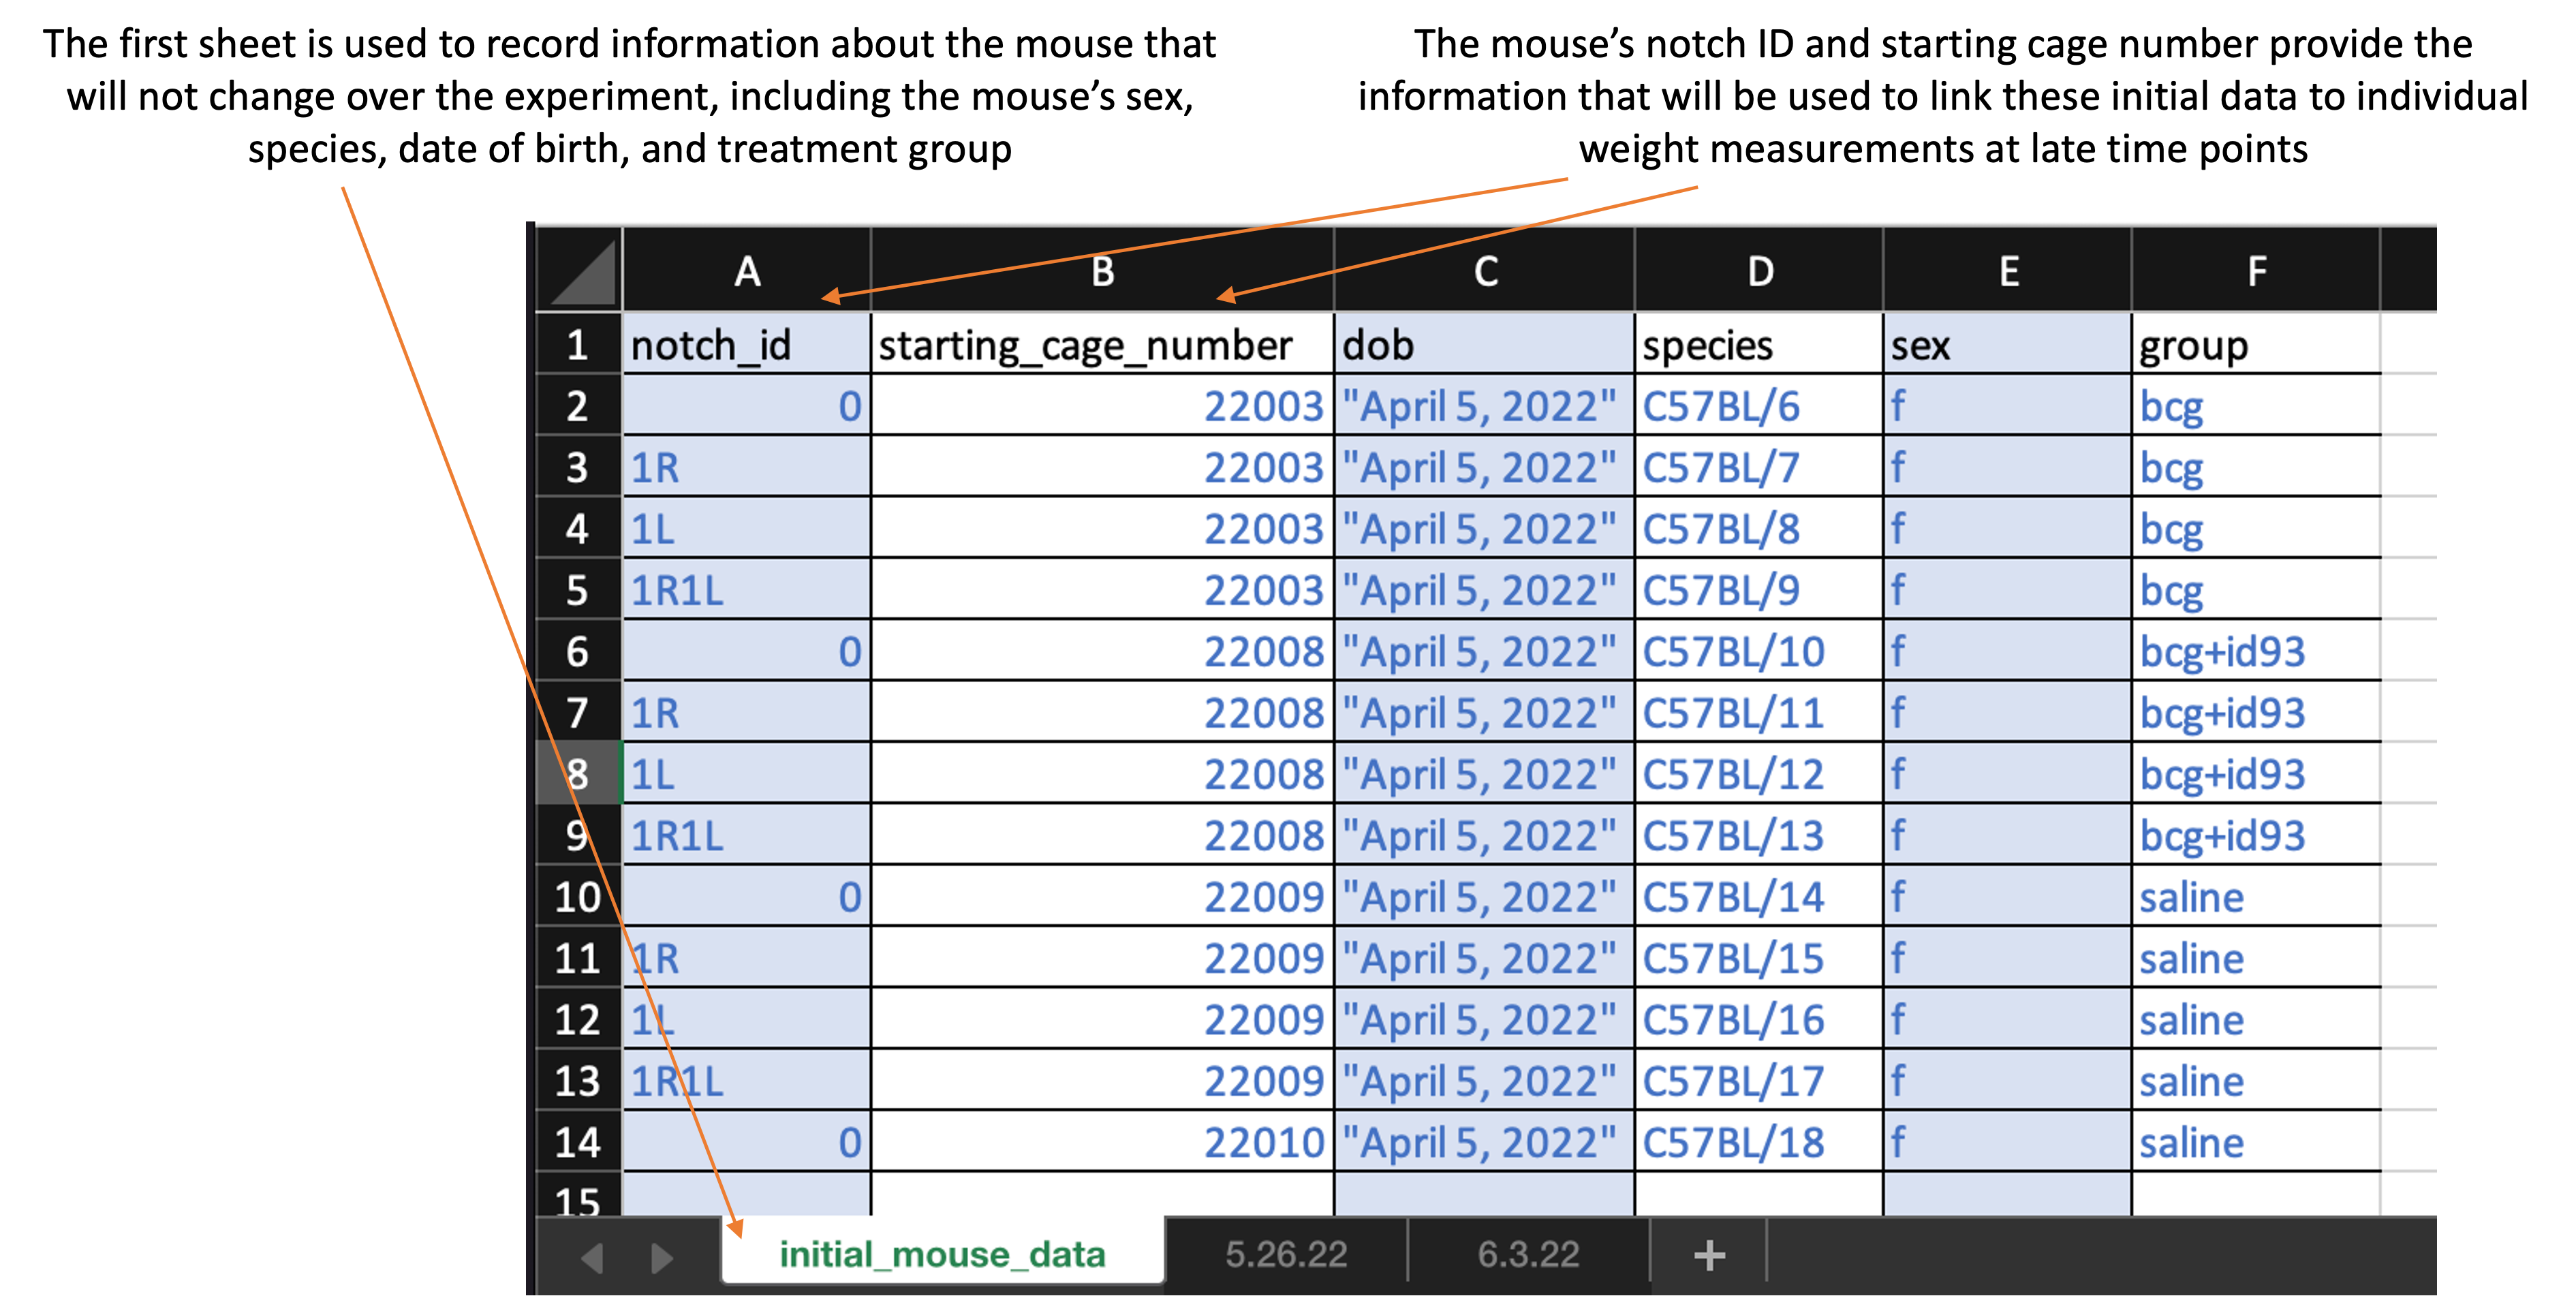
\includegraphics[width=1\linewidth]{figures/weight_template_initial}

The second and later sheets are used to record the weight at each measured timepoint.
The second sheet will record the weights on the first date they are measured, so
it should be recorded at the same time as the first sheet---with initial mouse
information---is completed. Here is what the first sheet of the template looks like:

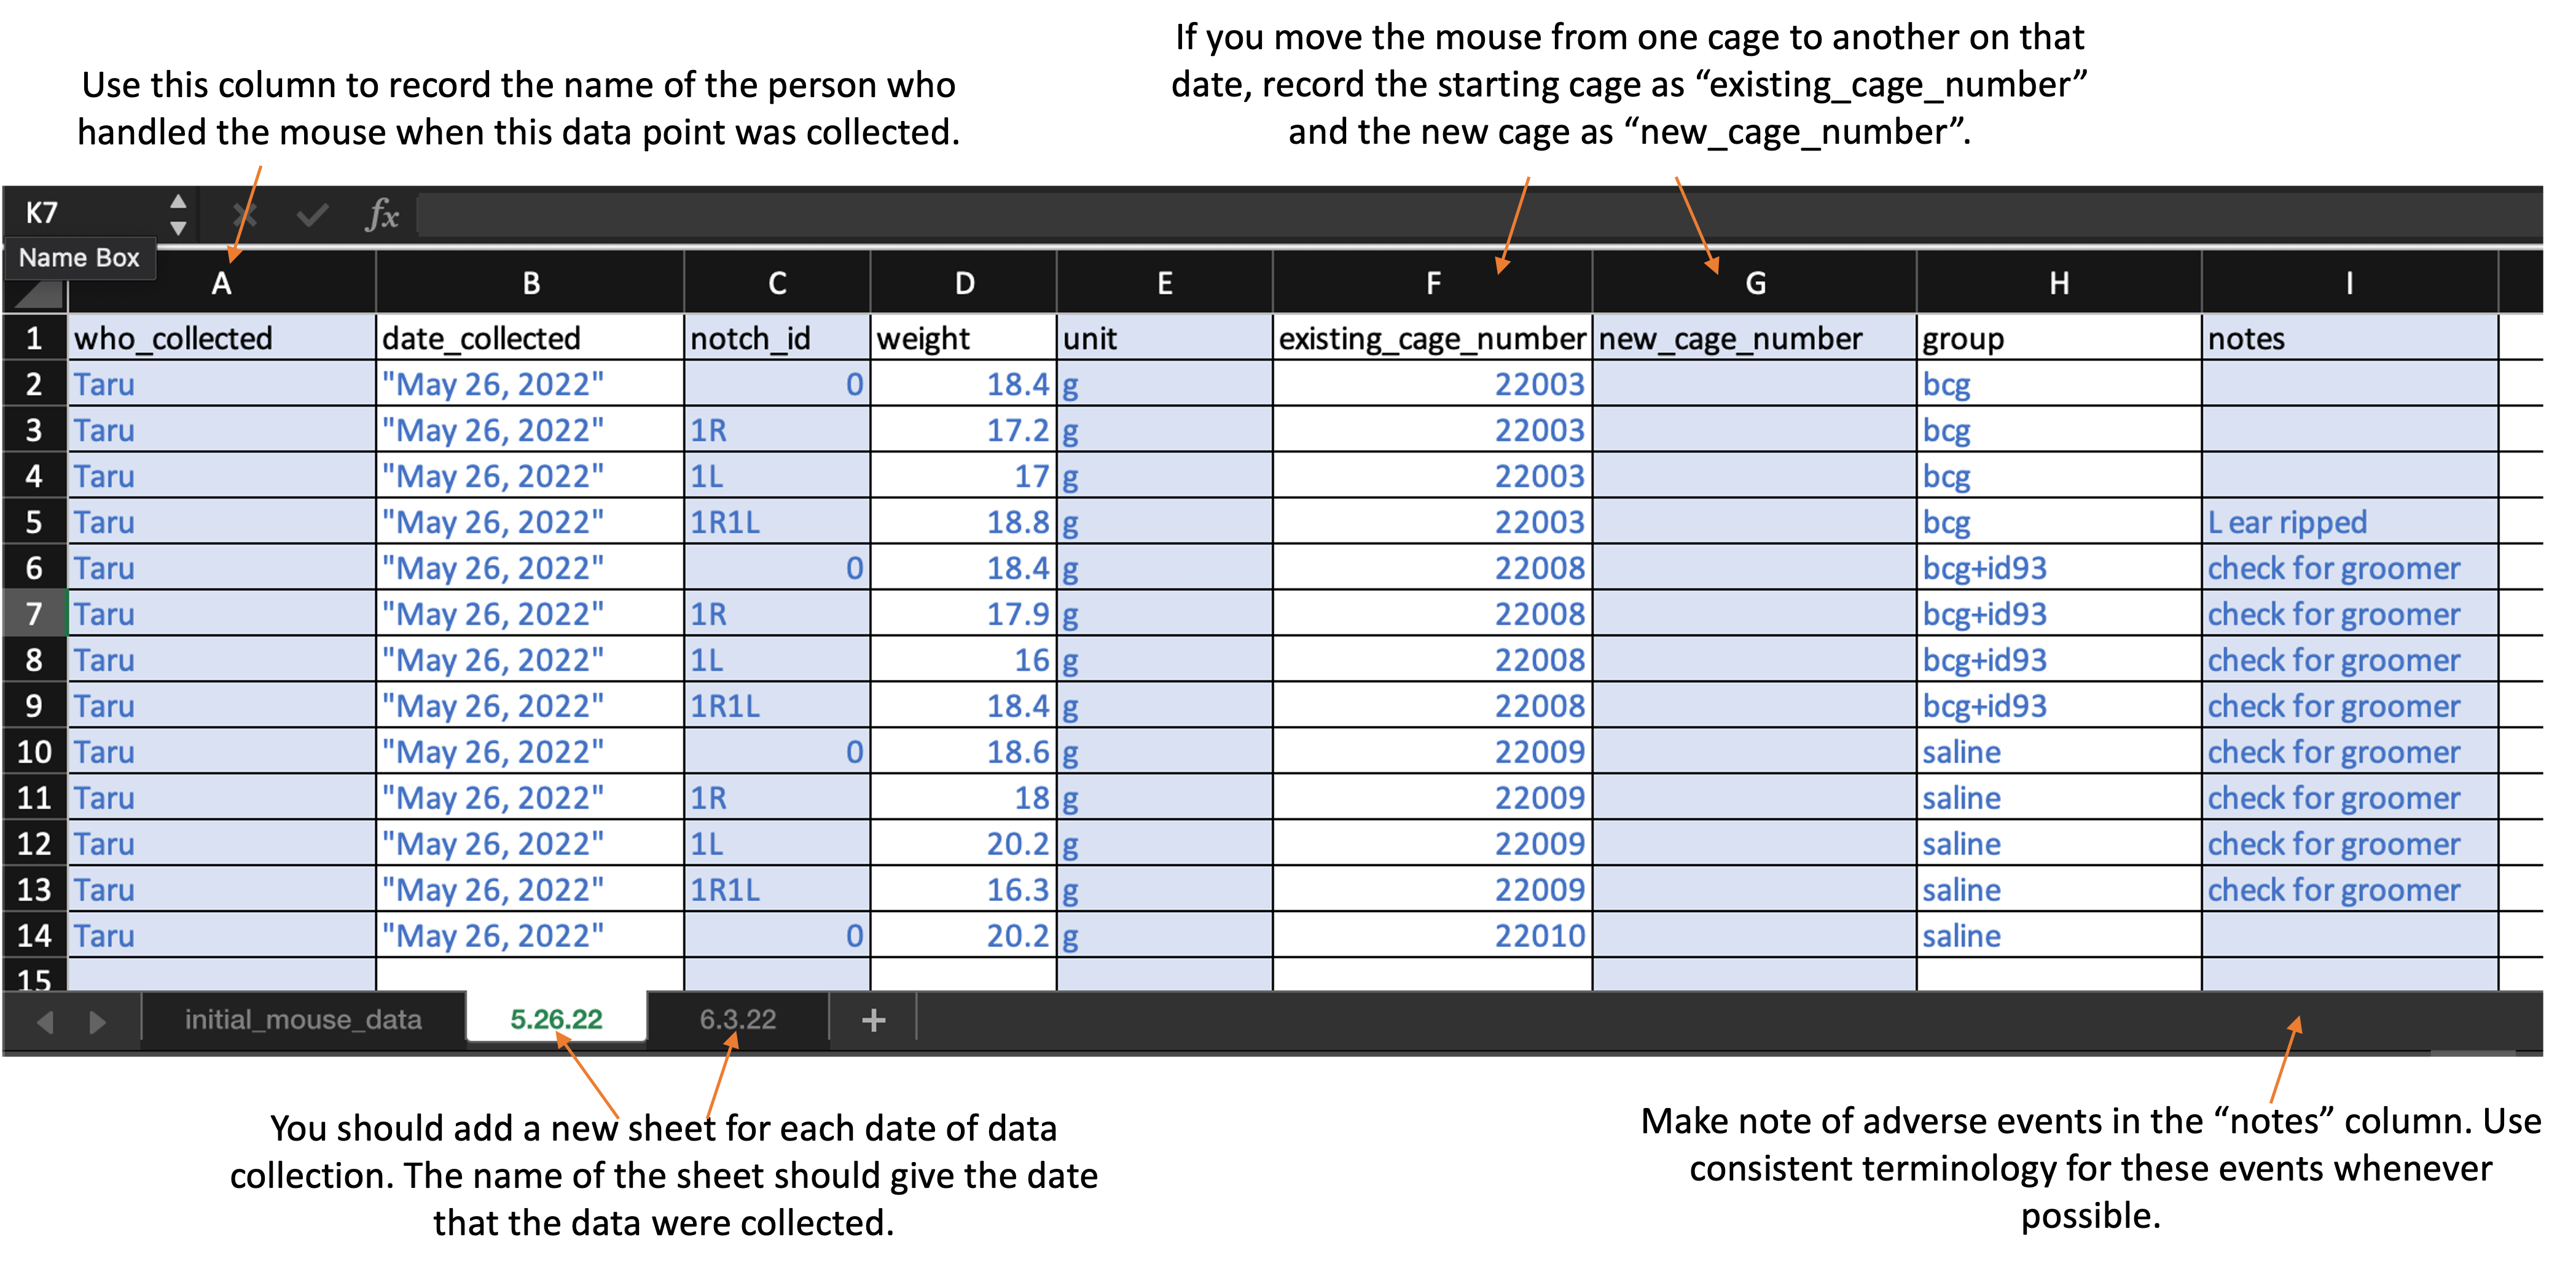
\includegraphics[width=1\linewidth]{figures/weight_template_page}

As you continue to measure at new timepoints, you should add a sheet at each
timepoint, with each new sheet following the format of the second sheet in the
template. The second and later sheets should be labeled with the date when those
weights were measured (e.g., ``5.26.22'' for weights measured on May 26, 2022).

When you download the template, it will have example values filled out in blue.
Use these to get an idea for how to record your own data. When you are ready
to record your own data, delete these example values and replace them with
data collected from your own experiment.

Column titles are as follows. First, in the first sheet, you will record:

\begin{itemize}
\tightlist
\item
  \texttt{notch\_id}: Record the ear notch pattern in the mouse. Make sure that you
  record consistently across all timepoints, so that each mouse can be tracked
  across dates. If you are doing single notches, for example, this might be ``0''
  for no notches, ``1R'' for one notch in the right ear, ``1L'' for one notch in the
  left ear, and ``1R1L'' for one notch in each ear.
\item
  \texttt{starting\_cage\_number}: Record the number of the cage that the mouse is put
  into at the start of the experiment. In combination with the mouse's \texttt{notch\_id},
  this will provide a unique identifier for each mouse at the start of the
  experiment.
\item
  \texttt{dob}: Record the date the mouse was born.
\item
  \texttt{species}: Record the species of the mouse (e.g., ``C57BL/6'' for C57 black 6 mice or
  ``CBA'' for CBA mice).
\item
  \texttt{sex}: Record as ``m'' for male or ``f'' for female
\item
  \texttt{group}: Provide the experimental group of the mouse. Be sure that you use the
  same abbreviation or notation across each timepoint. Examples of group
  designations might be: bcg, saline, bcg+id93, saline+id93, saline+noMtb
\end{itemize}

For the second and later sheets, you will record:

\begin{itemize}
\tightlist
\item
  \texttt{who\_collected}: Record the first name of the person who actually handled the mouse from the scale.
\item
  \texttt{date\_collected}: Record the date using quotation marks, with the month, then day, then year. For example, ``May 31, 2022''.
\item
  \texttt{weight}: Record as a number, without a unit in this column. The next column will be used for the units.\\
\item
  \texttt{unit}: Provide the units that were used to take the weight (e.g., ``g'' for grams). Be consistent across all animals and timepoints in the abbreviation that you use (e.g., always use ``g'' for grams, not ``g'' sometimes and ``grams'' sometimes)
\item
  \texttt{existing\_cage\_number}: Provide the cage number that the mouse is in when you start weighing at that time point. If the mouse is moved to another cage on this day, you will specify that in the next column. If the animal was moved from one cage to another between the last weighing and the date of the timepoint you are measuring, put in this column the cage number that the animal was in the last time it was weighed.
\item
  \texttt{new\_cage\_number}: If the animal is moved to a new cage on the date of the timepoint you are measuring, then use this column to record the number of the cage you move it too. Similarly, if the animal moved cages between the last measured timepoint and this one, use this column to record the cage it was moved to. Otherwise, if the animal stays in the same cage that it was at the last measured time point, leave this column empty.
\item
  \texttt{group}: Provide the experimental group of the mouse. Be sure that you use the same abbreviation or notation across each timepoint. Examples of group designations might be: bcg, saline, bcg+id93, saline+id93, saline+noMtb
\item
  \texttt{notes}: Record information regarding clinical observations (e.g., ``back is balding'', ``barbering'', ``excessive grooming'', ``euthanized'').
\end{itemize}

\hypertarget{processing-collected-data}{%
\subsection{Processing collected data}\label{processing-collected-data}}

Once data are collected, the file can be run through an R workflow. This workflow
will convert the data into a format that is easier to work with for data analysis
and visualization. It will also produce a report on the data in the spreadsheet, and
ultimately it will also write relevant results in a format that can be used
to populate a global database for all experiments in the project.

The next section provides the details of the pipeline. It aims to explain the
code that processes the data and generates visualizations. You do not need to
run this code step-by-step, but instead can access a script with the full
code \href{https://raw.githubusercontent.com/csu-impactb/CODING-TEAM-BOOKDOWN-/main/templates/report_templates/animal_weights.Rmd}{here}.

To use this reporting template, you need to download it to your computer and
save it in the file directory where you saved the data you collected with the
data collection template. You can then open RStudio and navigate so that you are
working within this directory. You should also make sure that you have installed
a few required packages on R on the computer you are using to run the report.
These packages are: \texttt{tidyverse}, \texttt{purrr}, \texttt{lubridate}, \texttt{readxl}, \texttt{knitr}, and
\texttt{ggbeeswarm}.

Within RStudio, open the report template file. There is one spot where you will
need to change the code in the template file, so it will read in the data from
the version of the template that you saved, which you may have renamed.
In the YAML of the report template file, change the file path beside ``data:''
so that it is the file name of your data file.

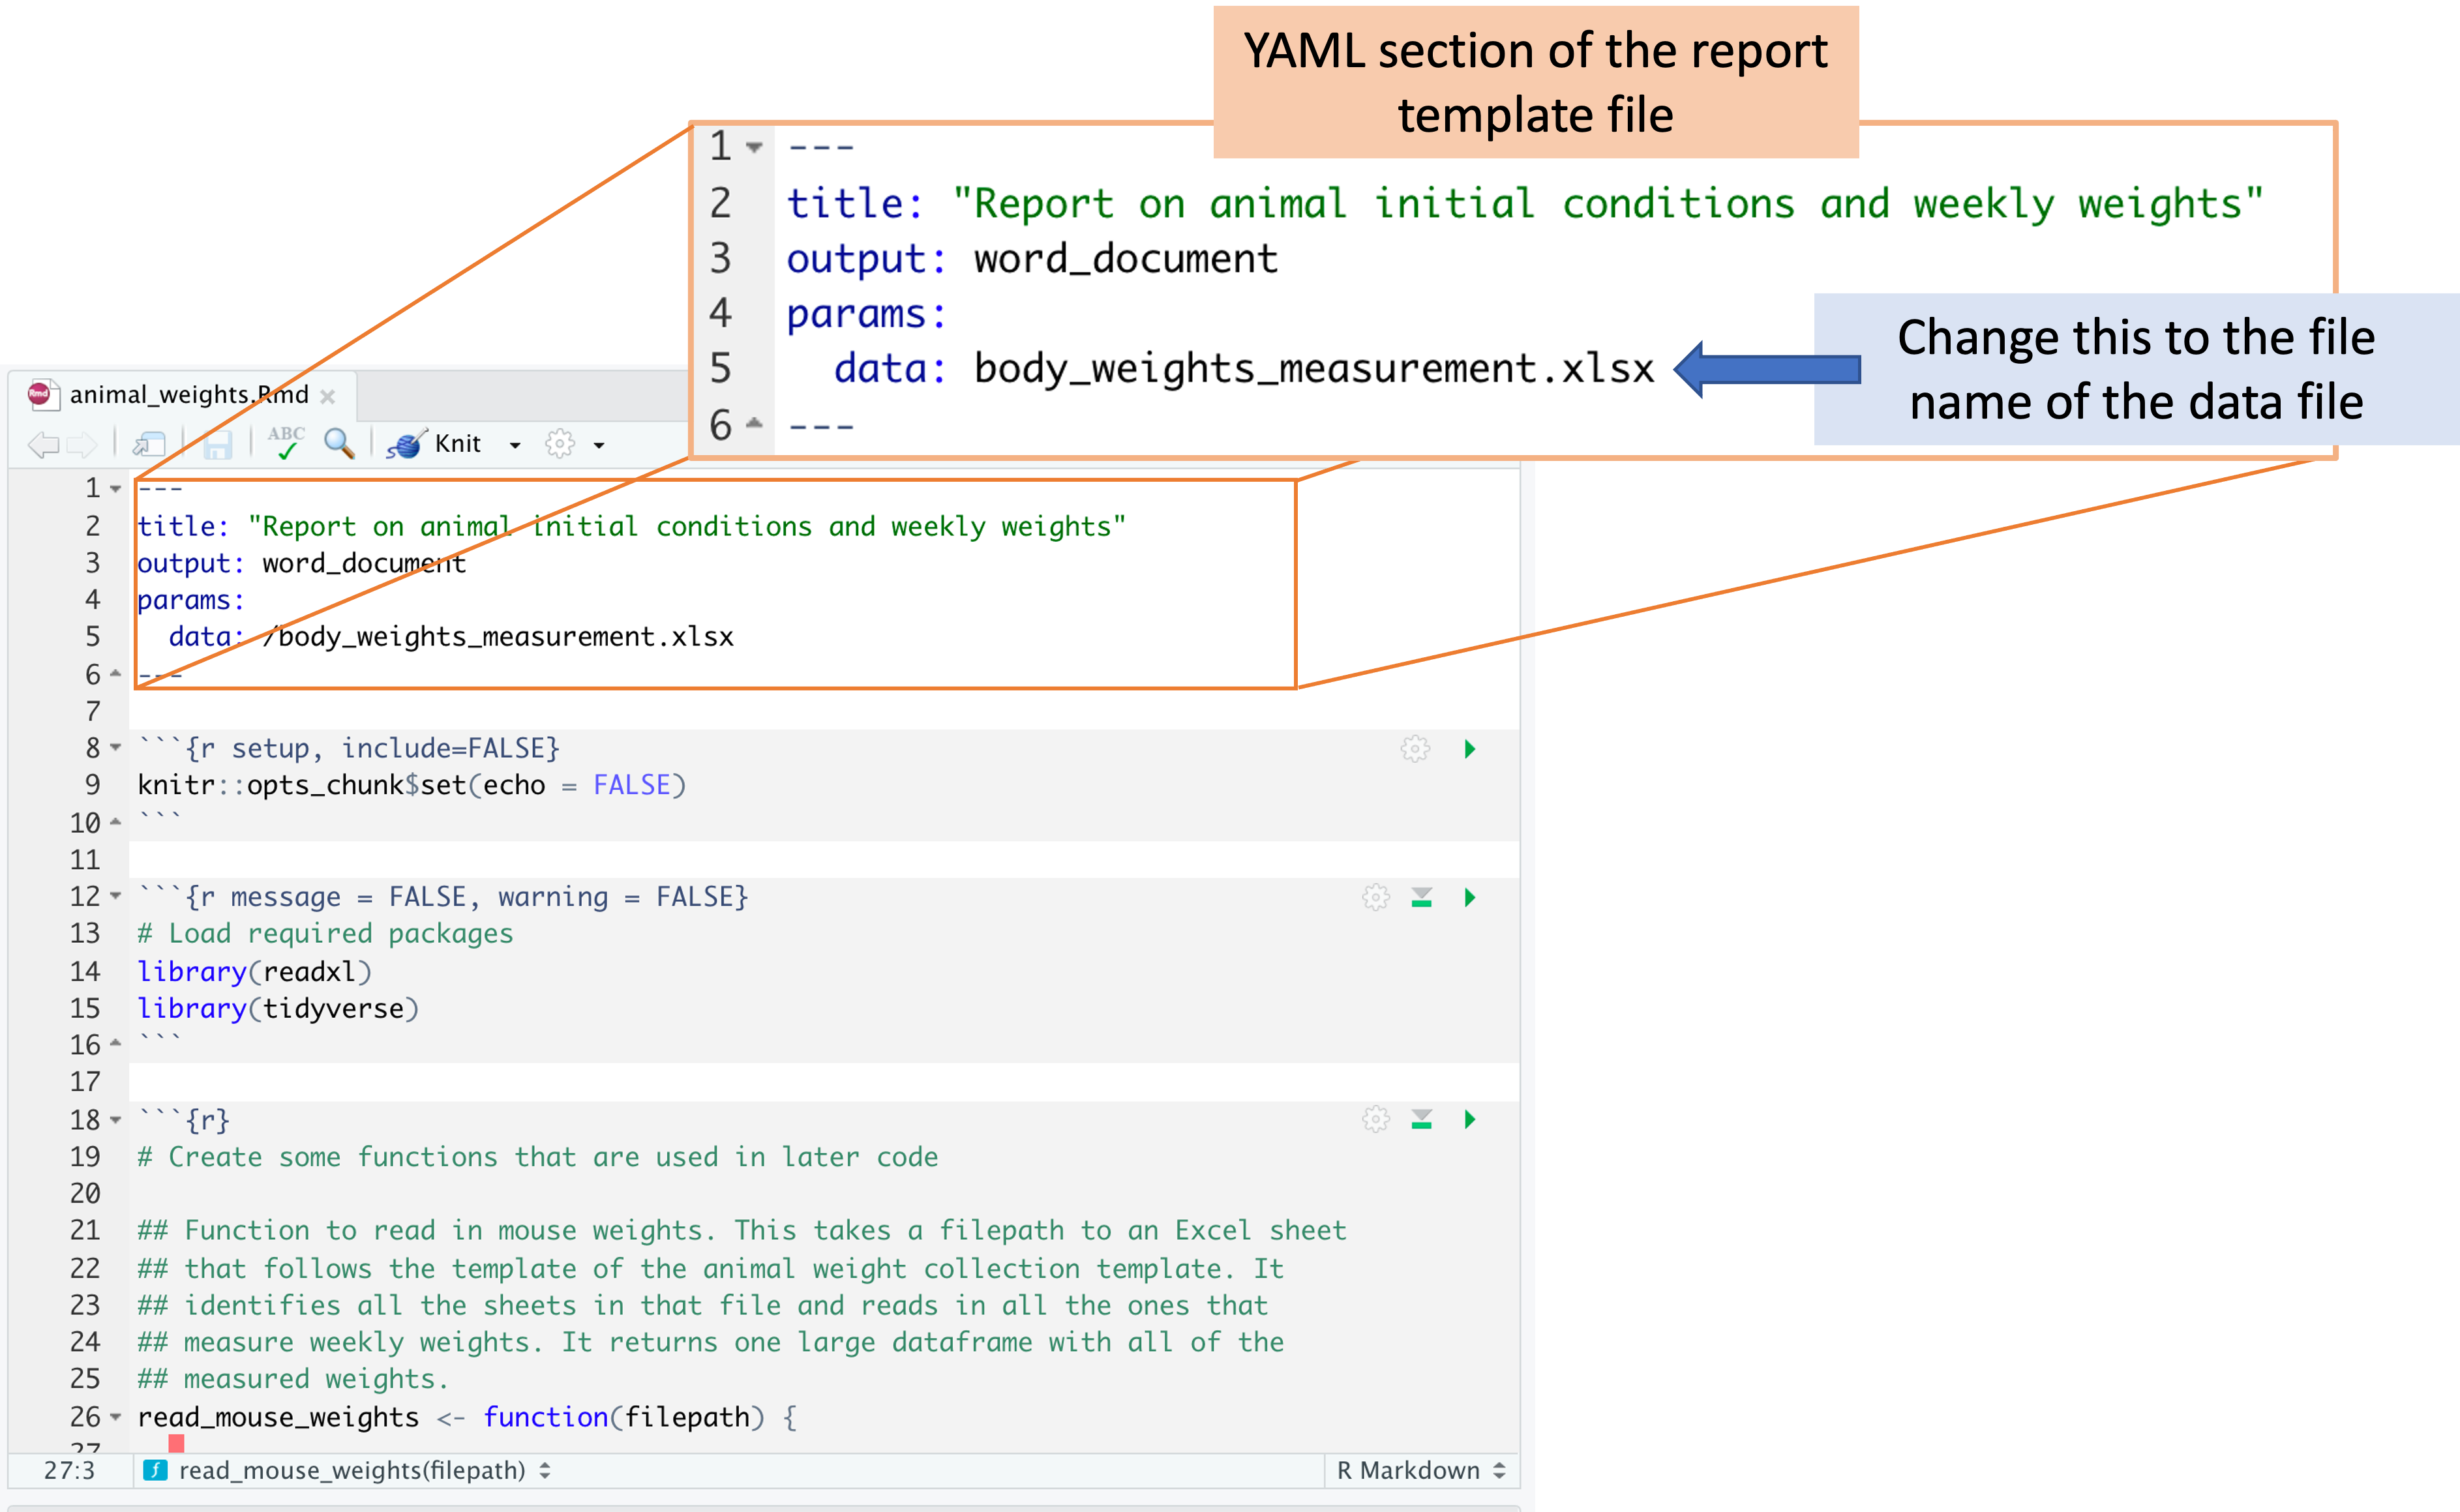
\includegraphics[width=1\linewidth]{figures/changing_file_path_weights_report_template}

Once you've made this change, you can use the ``Knit'' button in RStudio to
create a report from the data file and the report template file.

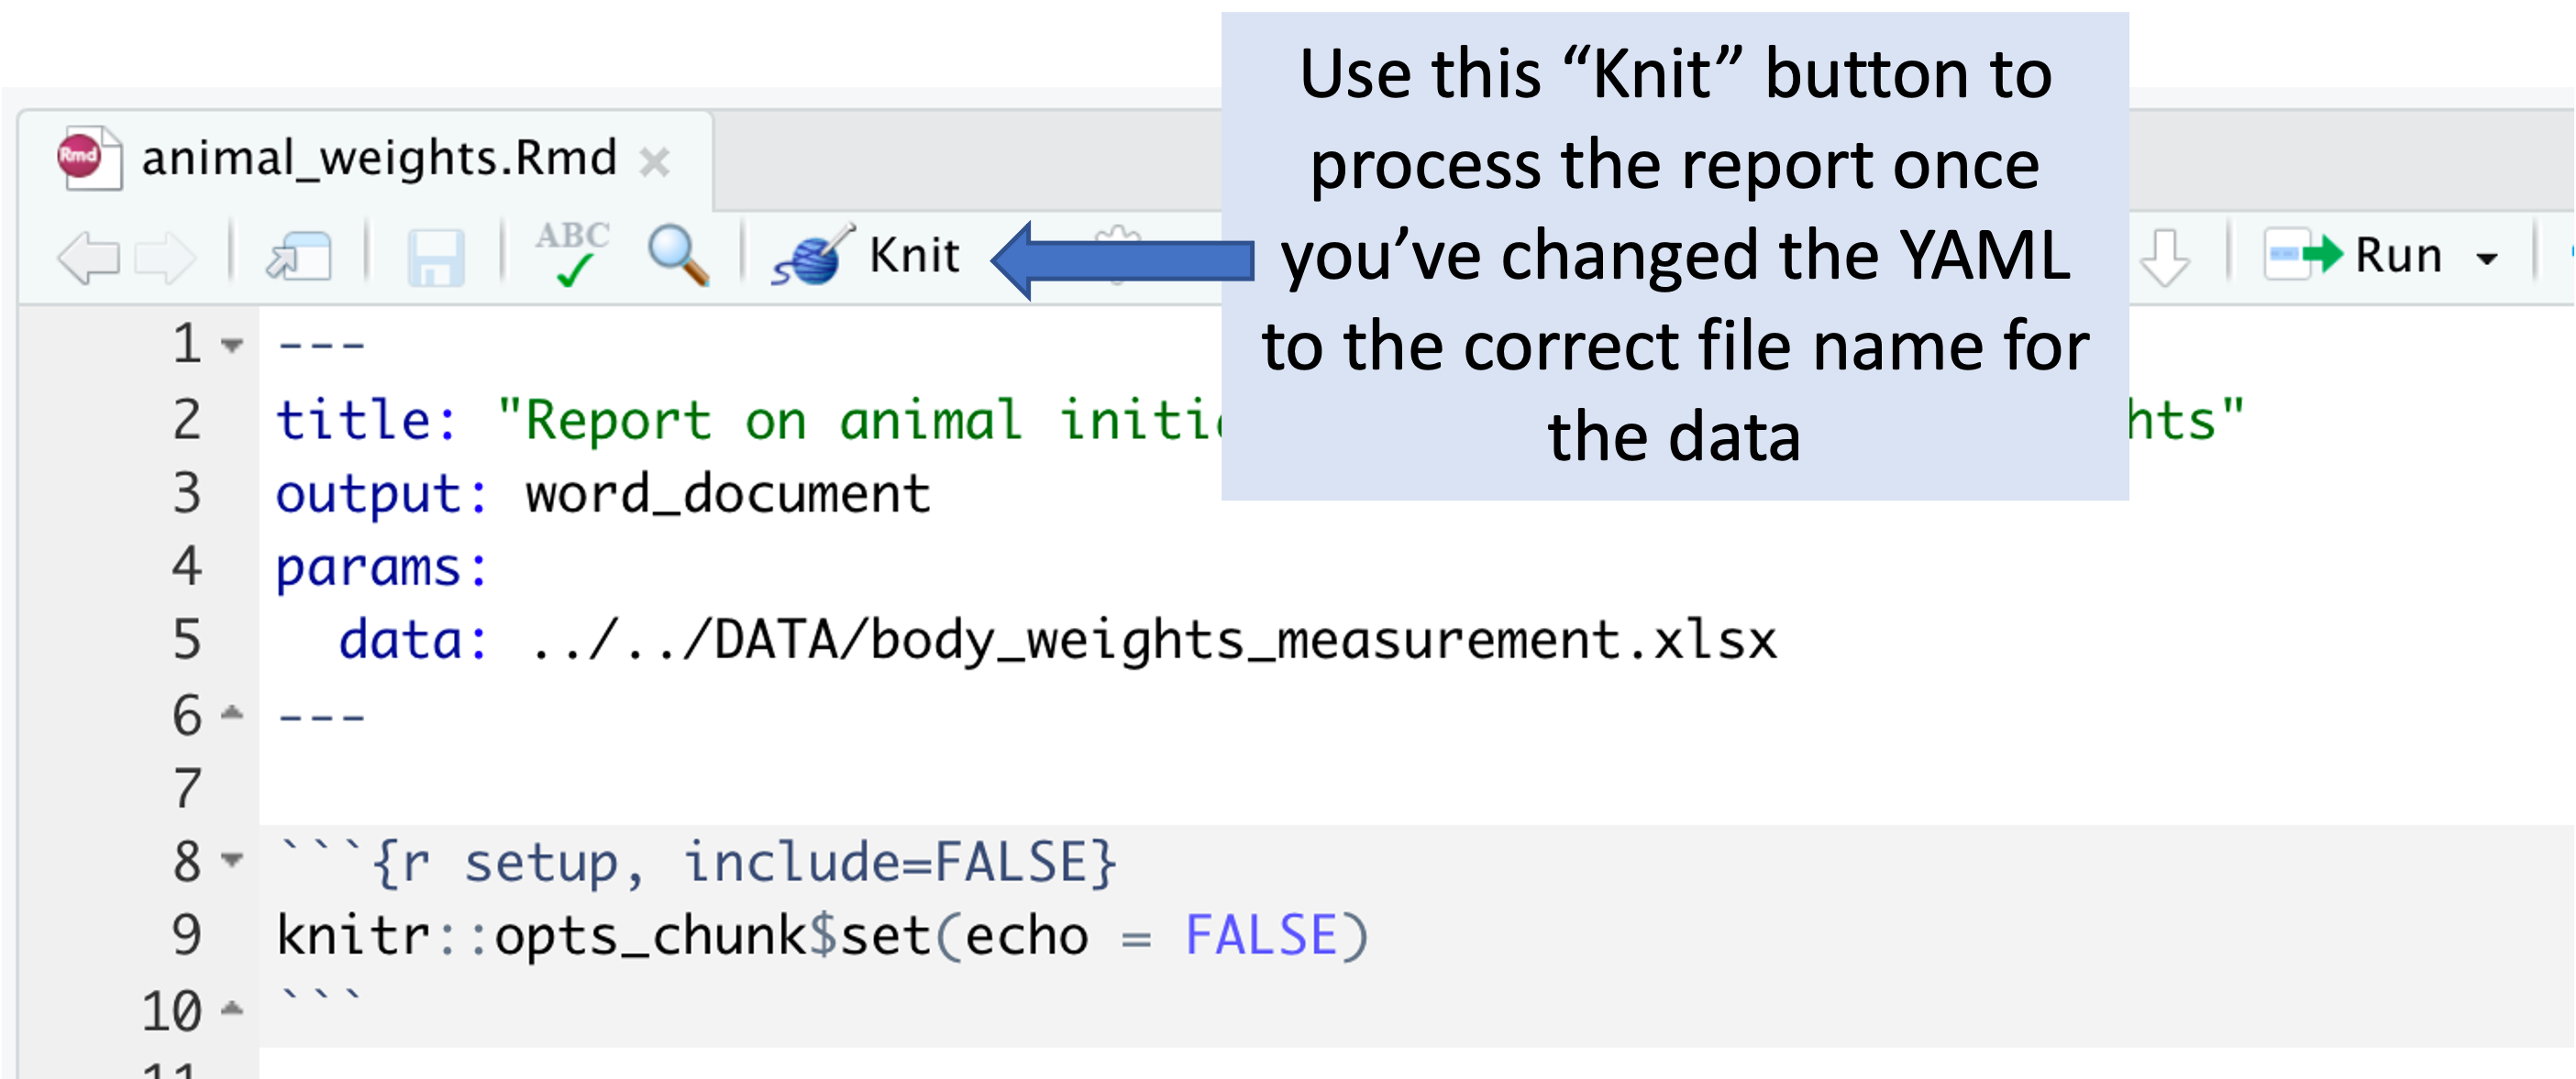
\includegraphics[width=1\linewidth]{figures/knit_button_for_weight_report}

The report includes the following elements:

\begin{itemize}
\tightlist
\item
  Summary table of animals at the start of the experiment
\item
  Time series plots of animal weights over the experiment, grouped by
  experimental group
\item
  Boxplots of the distribution of animal weights within each experimental
  group at the last available time point
\item
  Plot of measured weight, identified by the person who was handling the
  animal, to help determine if there are consistent differences by handler
\item
  Table of all the animals in the experiment at the last measured time point,
  ordered by their weight change since the previous measurement. This table
  is meant to help in identifying animals that may need to be euthanized for
  animal welfare reasons.
\end{itemize}

You can download an example of a report created using this template by
clicking \href{https://github.com/csu-impactb/CODING-TEAM-BOOKDOWN-/raw/main/templates/report_templates/animal_weights.docx}{here}.

When you knit to create the report, it will create a Word file in the
same file directory where you put your data file and report template.
It will also create and output a version of the data that has been
processed (in the case of the weights data, this mainly involves
tracking mice as they change cages, to link all weights that are from
a single animal). This output fill will be named ``\ldots{}'' and, like
the report file, will be saved in the same file directory as the
data file and the report template.

\hypertarget{details-of-processing-script}{%
\subsection{Details of processing script}\label{details-of-processing-script}}

This section goes through the code within the report template. It
explains each part of the code in detail. You do not need to understand
these details to use the report template. However, if you have questions
about how the data are being processed, or how the outputs are created,
all those details are available in this section.

As a note, there are two places in the following code where there's a small
change compared to the report template. In the report, you incorporate the path
to the data file using the \texttt{data:} section in the YAML at the top of the
document. In the following code, we've instead used the path of some example
data within this book's file directory, so the code will run for this chapter as
well.

First, the workflow loads some additional R libraries. You may need to install
these on your local R session if you do not already have them installed.

\begin{Shaded}
\begin{Highlighting}[]
\FunctionTok{library}\NormalTok{(readxl)}
\FunctionTok{library}\NormalTok{(tidyverse)}
\FunctionTok{library}\NormalTok{(ggbeeswarm)}
\end{Highlighting}
\end{Shaded}

These packages bring in some useful functions that are not available in the
base installation of R. They are all open source. To cite any of them, you
can use the \texttt{citation} function. For example, to get the information you would
need to cite the \texttt{readxl} package, in R you can run:

\begin{Shaded}
\begin{Highlighting}[]
\FunctionTok{citation}\NormalTok{(}\StringTok{"readxl"}\NormalTok{)}
\end{Highlighting}
\end{Shaded}

\begin{verbatim}
## 
## To cite package 'readxl' in publications use:
## 
##   Hadley Wickham and Jennifer Bryan (2019). readxl: Read Excel Files. R
##   package version 1.3.1. https://CRAN.R-project.org/package=readxl
## 
## A BibTeX entry for LaTeX users is
## 
##   @Manual{,
##     title = {readxl: Read Excel Files},
##     author = {Hadley Wickham and Jennifer Bryan},
##     year = {2019},
##     note = {R package version 1.3.1},
##     url = {https://CRAN.R-project.org/package=readxl},
##   }
\end{verbatim}

Next, the code in the report template creates a few custom functions to
help process the data from the data collection template. The first of these
functions checks the data collection template to identify all the timepoints
that were collected and then reads each in, ultimately joining data from
all time points into one large dataset.

The data collection template requires you to use a new sheet in the spreadsheet
for each weight collection time point, with a first sheet that records
initial information about the animals. If you only take weights at three
time points, there would only be three time point sheets in the final file.
Conversely, if you collect weight data at twenty time points, there would be
twenty sheets in the final file. The first function, called ``, reads the data file, checks
to find all the weight recording sheets, whether it's three or twenty, and then
reads the data in from all the sheets and binds them together into a single
dataframe.

\begin{Shaded}
\begin{Highlighting}[]
\DocumentationTok{\#\# Function to read in mouse weights. This takes a filepath to an Excel sheet}
\DocumentationTok{\#\# that follows the template of the animal weight collection template. It }
\DocumentationTok{\#\# identifies all the sheets in that file and reads in all the ones that }
\DocumentationTok{\#\# measure weekly weights. It returns one large dataframe with all of the }
\DocumentationTok{\#\# measured weights. }
\NormalTok{read\_mouse\_weights }\OtherTok{\textless{}{-}} \ControlFlowTok{function}\NormalTok{(filepath) \{}
  
  \CommentTok{\# getting info about all excel sheets}
\NormalTok{  mouse\_weights\_sheets }\OtherTok{\textless{}{-}}\NormalTok{ readxl}\SpecialCharTok{::}\FunctionTok{excel\_sheets}\NormalTok{(filepath)[}\SpecialCharTok{{-}}\DecValTok{1}\NormalTok{] }\CommentTok{\# First sheet is initial data, not mouse weights}
  
\NormalTok{  mouse\_weights }\OtherTok{\textless{}{-}}\NormalTok{ purrr}\SpecialCharTok{::}\FunctionTok{map}\NormalTok{(mouse\_weights\_sheets, }
                              \SpecialCharTok{\textasciitilde{}}\NormalTok{ readxl}\SpecialCharTok{::}\FunctionTok{read\_excel}\NormalTok{(filepath, }\AttributeTok{sheet =}\NormalTok{ .x, }
                                                   \AttributeTok{col\_types =} \FunctionTok{c}\NormalTok{(}\StringTok{"text"}\NormalTok{,   }\CommentTok{\# who\_collected}
                                                                 \StringTok{"text"}\NormalTok{,   }\CommentTok{\# date\_collected}
                                                                 \StringTok{"text"}\NormalTok{,   }\CommentTok{\# notch\_id}
                                                                 \StringTok{"numeric"}\NormalTok{, }\CommentTok{\# weight}
                                                                 \StringTok{"text"}\NormalTok{,   }\CommentTok{\# unit}
                                                                 \StringTok{"text"}\NormalTok{,   }\CommentTok{\# existing\_cage\_number}
                                                                 \StringTok{"text"}\NormalTok{,   }\CommentTok{\# new\_cage\_number}
                                                                 \StringTok{"text"}\NormalTok{,   }\CommentTok{\# group}
                                                                 \StringTok{"text"}    \CommentTok{\# notes}
\NormalTok{                                                                 ))) }\SpecialCharTok{\%\textgreater{}\%} 
\NormalTok{    dplyr}\SpecialCharTok{::}\FunctionTok{bind\_rows}\NormalTok{() }\SpecialCharTok{\%\textgreater{}\%} 
    \FunctionTok{mutate}\NormalTok{(}\AttributeTok{date\_collected =}\NormalTok{ lubridate}\SpecialCharTok{::}\FunctionTok{mdy}\NormalTok{(date\_collected))}

  \FunctionTok{return}\NormalTok{(mouse\_weights)}
\NormalTok{\}}
\end{Highlighting}
\end{Shaded}

The remaining functions are all functions to help track a mouse over the
experiment even if it changes cages. In processing this data, the key challenge
is to track a single mouse over the experiment. The mice are identified by a
pattern of notches in their ears. However, there are a limited number of notches
that can be distinguished, so the notch information does not distinctly identify
every mouse in the study, just every mouse within a certain cage. By knowing
both an ear notch ID and a cage number, you can distinctly identify each mouse
in the study.

However, mice are moved from one cage to another in some cases during a study.
If mice within a cage are fighting, or if they are showing signs of
excessive grooming, these can be reasons to move a mouse to a new cage once
the experiment has started. The cage moves need to be resolved when
processing the data so that each mouse can be tracked even as they move.

In the data collection template, we have created a design that aims to include
information about cage moves, but to do so in a way that is as simple as
possible for the person who is recording the data. The weights are recorded for
each time point in a separate sheet of the data collection template. On the
sheet for a time point, there are also columns to give the mouse's cage at the
start of that data collection time point, as well as the cage the mouse was
moved to, if it was moved. The report template code then uses this information
to create a unique ID for each mouse (one that is constant across the
experiment), and then attach it to the mouse's measurements even as the mouse is
moved from one cage to another. The following two functions both help with
this process:

\begin{Shaded}
\begin{Highlighting}[]
\CommentTok{\# Function to get the next cage number based on the }
\CommentTok{\# existing cage number and notch ID. If the mouse does not}
\CommentTok{\# switch cages again, the output is a vector of length 0. }
\CommentTok{\# This takes the dataframe and existing identifiers (notch id and}
\CommentTok{\# existing cage number) as inputs. It returns the next cage}
\CommentTok{\# that the mouse was moved to. If the mouse has not moved}
\CommentTok{\# from the existing case, the output has length 0.}
\NormalTok{get\_next\_cage }\OtherTok{\textless{}{-}} \ControlFlowTok{function}\NormalTok{(existing\_cage\_number, notch\_id, }
                          \AttributeTok{df =}\NormalTok{ our\_mouse\_weights)\{}
\NormalTok{  next\_cage }\OtherTok{\textless{}{-}}\NormalTok{ df }\SpecialCharTok{\%\textgreater{}\%} 
    \FunctionTok{filter}\NormalTok{(.data}\SpecialCharTok{$}\NormalTok{existing\_cage\_number }\SpecialCharTok{==}\NormalTok{ \{\{existing\_cage\_number\}\} }\SpecialCharTok{\&}
\NormalTok{             .data}\SpecialCharTok{$}\NormalTok{notch\_id }\SpecialCharTok{==}\NormalTok{ \{\{notch\_id\}\} }\SpecialCharTok{\&} 
             \SpecialCharTok{!}\FunctionTok{is.na}\NormalTok{(.data}\SpecialCharTok{$}\NormalTok{new\_cage\_number)) }\SpecialCharTok{\%\textgreater{}\%} 
    \FunctionTok{pull}\NormalTok{(new\_cage\_number)}
  
  \FunctionTok{return}\NormalTok{(next\_cage)}
\NormalTok{\}}

\CommentTok{\# Function to get the full list of cages for each individual }
\CommentTok{\# mouse, over the course of all data collected to date. This }
\CommentTok{\# inputs the starting identifiers of the mouse (starting cage ID }
\CommentTok{\# and notch ID). It then works through any cage changes to create}
\CommentTok{\# a list for that mouse of all cages it was put in over the }
\CommentTok{\# course of the experiment. }
\NormalTok{get\_mouse\_cages }\OtherTok{\textless{}{-}} \ControlFlowTok{function}\NormalTok{(mouse\_starting\_cage, mouse\_notch\_id, }
                            \AttributeTok{df =}\NormalTok{ our\_mouse\_weights)\{}
\NormalTok{  mouse\_cage\_list }\OtherTok{\textless{}{-}}\NormalTok{ mouse\_starting\_cage}
\NormalTok{  i }\OtherTok{\textless{}{-}} \DecValTok{1}
  
  \ControlFlowTok{while}\NormalTok{(}\ConstantTok{TRUE}\NormalTok{)\{}
\NormalTok{    next\_cage }\OtherTok{\textless{}{-}} \FunctionTok{get\_next\_cage}\NormalTok{(}\AttributeTok{existing\_cage\_number =}
\NormalTok{                               mouse\_cage\_list[i],}
                               \AttributeTok{notch\_id =}\NormalTok{ mouse\_notch\_id, }
                               \AttributeTok{df =}\NormalTok{ df)}
    \ControlFlowTok{if}\NormalTok{(}\FunctionTok{length}\NormalTok{(next\_cage) }\SpecialCharTok{==} \DecValTok{0}\NormalTok{) \{}
      \ControlFlowTok{break}
\NormalTok{      \}}
\NormalTok{    i }\OtherTok{\textless{}{-}}\NormalTok{ i }\SpecialCharTok{+} \DecValTok{1}
\NormalTok{    mouse\_cage\_list[i] }\OtherTok{\textless{}{-}}\NormalTok{ next\_cage}
\NormalTok{    \}}
  
  \FunctionTok{return}\NormalTok{(mouse\_cage\_list)}
\NormalTok{\}}
\end{Highlighting}
\end{Shaded}

Next, the report template code gets to the workflow itself, where it uses
both these custom functions and other R code to process the data and then
to provide summaries and visualizations of the data.

The first step in the workflow is to read in the data from the spreadsheet.
As long as the data are collected following the template that was described
earlier, this code should be able to read it in correctly and create a
master dataset with the data from all sheets of the spreadsheet. This step
of the pipeline uses one of the custom functions that was defined at the start
of the report template code:

\begin{Shaded}
\begin{Highlighting}[]
\CommentTok{\# Read in the mouse weights from the Excel template. This creates one large}
\CommentTok{\# dataframe with the weights from all the timepoints. }
\NormalTok{our\_mouse\_weights }\OtherTok{\textless{}{-}} \FunctionTok{read\_mouse\_weights}\NormalTok{(}\AttributeTok{filepath =}
                                          \StringTok{"DATA/body\_weights\_measurement.xlsx"}\NormalTok{)}
\end{Highlighting}
\end{Shaded}

Next, the code runs through a number of steps to create a unique ID for
each mouse and then apply that ID to each time point, even if a mouse
changes cages.

\begin{Shaded}
\begin{Highlighting}[]
\CommentTok{\# Add a unique mouse ID for the first time point. This will become each mouse\textquotesingle{}s}
\CommentTok{\# unique ID across all measured timepoints.}
\NormalTok{our\_mouse\_weights }\OtherTok{\textless{}{-}}\NormalTok{ our\_mouse\_weights }\SpecialCharTok{\%\textgreater{}\%} 
  \FunctionTok{mutate}\NormalTok{(}\AttributeTok{mouse\_id =} \DecValTok{1}\SpecialCharTok{:}\FunctionTok{n}\NormalTok{(), }
         \AttributeTok{mouse\_id =} \FunctionTok{ifelse}\NormalTok{(date\_collected }\SpecialCharTok{==}
                                    \FunctionTok{first}\NormalTok{(date\_collected), }
\NormalTok{                                  mouse\_id, }
                                  \ConstantTok{NA}\NormalTok{))}

\CommentTok{\# Create a dataframe that lists all mice at the first time point, }
\CommentTok{\# as well as a list of all the cages they have been in over the}
\CommentTok{\# experiment}
\NormalTok{mice\_cage\_lists }\OtherTok{\textless{}{-}}\NormalTok{ our\_mouse\_weights }\SpecialCharTok{\%\textgreater{}\%} 
  \FunctionTok{filter}\NormalTok{(date\_collected }\SpecialCharTok{==} \FunctionTok{first}\NormalTok{(date\_collected)) }\SpecialCharTok{\%\textgreater{}\%} 
  \FunctionTok{select}\NormalTok{(notch\_id, existing\_cage\_number, mouse\_id) }\SpecialCharTok{\%\textgreater{}\%} 
  \FunctionTok{mutate}\NormalTok{(}\AttributeTok{cage\_list =} \FunctionTok{map2}\NormalTok{(}\AttributeTok{.x =}\NormalTok{ existing\_cage\_number, }
                          \AttributeTok{.y =}\NormalTok{ notch\_id, }
                          \AttributeTok{.f =} \SpecialCharTok{\textasciitilde{}} \FunctionTok{get\_mouse\_cages}\NormalTok{(.x, .y, }\AttributeTok{df =}\NormalTok{ our\_mouse\_weights)))}

\CommentTok{\# Add a column with the latest cage to the weight dataframe}
\NormalTok{our\_mouse\_weights}\SpecialCharTok{$}\NormalTok{latest\_cage }\OtherTok{\textless{}{-}} \ConstantTok{NA}

\CommentTok{\# Loop through all the individual mice, based on mice with a }
\CommentTok{\# measurement at the first time point. Add the unique ID for }
\CommentTok{\# each mouse, which will apply throughout the experiment. Also }
\CommentTok{\# add the most recent cage ID, so the mouse can be identified}
\CommentTok{\# by lab members based on it\textquotesingle{}s current location}
\ControlFlowTok{for}\NormalTok{(i }\ControlFlowTok{in} \DecValTok{1}\SpecialCharTok{:}\FunctionTok{nrow}\NormalTok{(mice\_cage\_lists))\{}
\NormalTok{  this\_notch\_id }\OtherTok{\textless{}{-}}\NormalTok{ mice\_cage\_lists[i, ]}\SpecialCharTok{$}\NormalTok{notch\_id}
\NormalTok{  this\_cage\_list }\OtherTok{\textless{}{-}}\NormalTok{ mice\_cage\_lists[i, ]}\SpecialCharTok{$}\NormalTok{cage\_list[[}\DecValTok{1}\NormalTok{]]}
\NormalTok{  this\_unique\_id }\OtherTok{\textless{}{-}}\NormalTok{ mice\_cage\_lists[i, ]}\SpecialCharTok{$}\NormalTok{mouse\_id}
\NormalTok{  latest\_cage }\OtherTok{\textless{}{-}}\NormalTok{ this\_cage\_list[}\FunctionTok{length}\NormalTok{(this\_cage\_list)]}
  
\NormalTok{  our\_mouse\_weights}\SpecialCharTok{$}\NormalTok{mouse\_id[our\_mouse\_weights}\SpecialCharTok{$}\NormalTok{notch\_id }\SpecialCharTok{==}\NormalTok{ this\_notch\_id }\SpecialCharTok{\&} 
\NormalTok{                       our\_mouse\_weights}\SpecialCharTok{$}\NormalTok{existing\_cage\_number }\SpecialCharTok{\%in\%} 
\NormalTok{                       this\_cage\_list] }\OtherTok{\textless{}{-}}\NormalTok{ this\_unique\_id}
  
\NormalTok{  our\_mouse\_weights}\SpecialCharTok{$}\NormalTok{latest\_cage[our\_mouse\_weights}\SpecialCharTok{$}\NormalTok{notch\_id }\SpecialCharTok{==}\NormalTok{ this\_notch\_id }\SpecialCharTok{\&} 
\NormalTok{                       our\_mouse\_weights}\SpecialCharTok{$}\NormalTok{existing\_cage\_number }\SpecialCharTok{\%in\%} 
\NormalTok{                       this\_cage\_list] }\OtherTok{\textless{}{-}}\NormalTok{ latest\_cage}
\NormalTok{\}}

\CommentTok{\# Add a label for each mouse based on its notch\_id and latest cage}
\NormalTok{our\_mouse\_weights }\OtherTok{\textless{}{-}}\NormalTok{ our\_mouse\_weights }\SpecialCharTok{\%\textgreater{}\%} 
  \FunctionTok{mutate}\NormalTok{(}\AttributeTok{mouse\_label =} \FunctionTok{paste}\NormalTok{(}\StringTok{"Cage:"}\NormalTok{, latest\_cage, }
                             \StringTok{"Notch:"}\NormalTok{, notch\_id))}
\end{Highlighting}
\end{Shaded}

Ultimately, this creates both a unique ID for each mouse (in a column of the
dataframe called \texttt{mouse\_id}), as well as creates a unique label that can be used
in plots and tables (given in the \texttt{mouse\_label} column). The unique ID is set at
the beginning of the study for each mouse and remains the same throughout the
study. The label, on the other hand, is based on the mouse's ear notch pattern
and the most recent cage it was recorded to be in. We made this choice for a
labeling identifier, because it will help the researchers to quickly identify a
mouse in the study based on it's current, rather than starting, cage.

The next part of the code reads in the initial data that were recorded for each
animal in the experiment. The code then pulls in information from the processed
weights dataset to match these initial data with each animals unique ID.
Ultimately, these starting data are incorporated into the large dataset of mouse
weights, creating a single large dataset to work with (\texttt{our\_mouse\_weights}) that
includes all the information that was recorded in the data collection template.

\begin{Shaded}
\begin{Highlighting}[]
\CommentTok{\# Read in the data from the original file with the initial animal }
\CommentTok{\# characteristics}
\NormalTok{mouse\_initial }\OtherTok{\textless{}{-}}\NormalTok{ readxl}\SpecialCharTok{::}\FunctionTok{read\_excel}\NormalTok{(}\StringTok{"DATA/body\_weights\_measurement.xlsx"}\NormalTok{, }
                                      \AttributeTok{sheet =} \DecValTok{1}\NormalTok{, }
                                      \AttributeTok{col\_types =} \FunctionTok{c}\NormalTok{(}\StringTok{"text"}\NormalTok{, }\CommentTok{\# notch\_id}
                                                    \StringTok{"text"}\NormalTok{, }\CommentTok{\# starting\_cage\_number}
                                                    \StringTok{"text"}\NormalTok{, }\CommentTok{\# dob}
                                                    \StringTok{"text"}\NormalTok{, }\CommentTok{\# species}
                                                    \StringTok{"text"}\NormalTok{, }\CommentTok{\# sex}
                                                    \StringTok{"text"} \CommentTok{\# group}
\NormalTok{                                                    )) }\SpecialCharTok{\%\textgreater{}\%}
  \FunctionTok{mutate}\NormalTok{(}\AttributeTok{dob =}\NormalTok{ lubridate}\SpecialCharTok{::}\FunctionTok{mdy}\NormalTok{(dob), }
         \AttributeTok{sex =}\NormalTok{ forcats}\SpecialCharTok{::}\FunctionTok{as\_factor}\NormalTok{(sex))}

\CommentTok{\# Figure out the starting cage for each mouse, so they can be incorporated}
\CommentTok{\# with the initial data so we can get the mouse ID that was added for the }
\CommentTok{\# starting time point}
\NormalTok{mouse\_ids }\OtherTok{\textless{}{-}}\NormalTok{ our\_mouse\_weights }\SpecialCharTok{\%\textgreater{}\%} 
  \FunctionTok{filter}\NormalTok{(date\_collected }\SpecialCharTok{==} \FunctionTok{first}\NormalTok{(date\_collected)) }\SpecialCharTok{\%\textgreater{}\%} 
  \FunctionTok{select}\NormalTok{(notch\_id, existing\_cage\_number, mouse\_id) }\SpecialCharTok{\%\textgreater{}\%} 
  \FunctionTok{rename}\NormalTok{(}\AttributeTok{starting\_cage\_number =}\NormalTok{ existing\_cage\_number)}

\CommentTok{\# Merge in the mouse IDs with the dataframe of initial mouse characteristics}
\NormalTok{mouse\_initial }\OtherTok{\textless{}{-}}\NormalTok{ mouse\_initial }\SpecialCharTok{\%\textgreater{}\%} 
  \FunctionTok{left\_join}\NormalTok{(mouse\_ids, }\AttributeTok{by =} \FunctionTok{c}\NormalTok{(}\StringTok{"notch\_id"}\NormalTok{, }\StringTok{"starting\_cage\_number"}\NormalTok{))}

\CommentTok{\# Join the initial data with the weekly weights data into one large dataset}
\NormalTok{our\_mouse\_weights }\OtherTok{\textless{}{-}}\NormalTok{ our\_mouse\_weights }\SpecialCharTok{\%\textgreater{}\%} 
  \FunctionTok{left\_join}\NormalTok{(mouse\_initial, }\AttributeTok{by =} \FunctionTok{c}\NormalTok{(}\StringTok{"mouse\_id"}\NormalTok{, }\StringTok{"notch\_id"}\NormalTok{, }\StringTok{"group"}\NormalTok{))}
\end{Highlighting}
\end{Shaded}

At this point, the first few rows of this large dataset look like this:

\begin{Shaded}
\begin{Highlighting}[]
\NormalTok{our\_mouse\_weights }\SpecialCharTok{\%\textgreater{}\%} 
  \FunctionTok{slice}\NormalTok{(}\DecValTok{1}\SpecialCharTok{:}\DecValTok{5}\NormalTok{)}
\end{Highlighting}
\end{Shaded}

\begin{verbatim}
## # A tibble: 5 x 16
##   who_collected date_collected notch_id weight unit  existing_cage_number
##   <chr>         <date>         <chr>     <dbl> <chr> <chr>               
## 1 Taru          2022-05-26     0          18.4 g     22003               
## 2 Taru          2022-05-26     1R         17.2 g     22003               
## 3 Taru          2022-05-26     1L         17   g     22003               
## 4 Taru          2022-05-26     1R1L       18.8 g     22003               
## 5 Taru          2022-05-26     0          18.4 g     22004               
## # ... with 10 more variables: new_cage_number <chr>, group <chr>, notes <chr>,
## #   mouse_id <int>, latest_cage <chr>, mouse_label <chr>,
## #   starting_cage_number <chr>, dob <date>, species <chr>, sex <fct>
\end{verbatim}

The rest of the code in the report template will create summaries and graphs of the
data. First, there is some code that provides summaries of the research animals at
the start of the experiment. It uses the \texttt{mouse\_initial} dataset (which pulled
in data from the first sheet of the data collection template). It uses a
\texttt{summarize} call to summarize details from this sheet of data, including the
species of the animal, the total number of animals, how many were males versus
females, and which experimental groups were included. It uses some additional
code to format the data so the resulting table will be clearer, and then
uses the \texttt{kable} function to output the results as a nicely formatted table.

\begin{Shaded}
\begin{Highlighting}[]
\CommentTok{\# Create a table that summarizes the animals at the start of the experiment}
\NormalTok{mouse\_initial }\SpecialCharTok{\%\textgreater{}\%} 
  \FunctionTok{summarize}\NormalTok{(}\AttributeTok{Species =} \FunctionTok{paste}\NormalTok{(}\FunctionTok{unique}\NormalTok{(species), }\AttributeTok{collapse =} \StringTok{", "}\NormalTok{), }
            \StringTok{\textasciigrave{}}\AttributeTok{Total animals}\StringTok{\textasciigrave{}} \OtherTok{=} \FunctionTok{n}\NormalTok{(), }
            \StringTok{\textasciigrave{}}\AttributeTok{Sex distribution}\StringTok{\textasciigrave{}} \OtherTok{=} \FunctionTok{paste0}\NormalTok{(}\StringTok{"male: "}\NormalTok{, }\FunctionTok{sum}\NormalTok{(sex }\SpecialCharTok{==} \StringTok{"m"}\NormalTok{), }
                                      \StringTok{", female: "}\NormalTok{, }\FunctionTok{sum}\NormalTok{(sex }\SpecialCharTok{==} \StringTok{"f"}\NormalTok{)),}
            \StringTok{\textasciigrave{}}\AttributeTok{Experimental groups}\StringTok{\textasciigrave{}} \OtherTok{=} \FunctionTok{paste}\NormalTok{(}\FunctionTok{unique}\NormalTok{(group), }\AttributeTok{collapse =} \StringTok{", "}\NormalTok{),}
            \StringTok{\textasciigrave{}}\AttributeTok{N. of starting cages}\StringTok{\textasciigrave{}} \OtherTok{=}
              \FunctionTok{length}\NormalTok{(}\FunctionTok{unique}\NormalTok{(starting\_cage\_number))) }\SpecialCharTok{\%\textgreater{}\%} 
  \FunctionTok{mutate\_all}\NormalTok{(as.character) }\SpecialCharTok{\%\textgreater{}\%} 
  \FunctionTok{pivot\_longer}\NormalTok{(}\FunctionTok{everything}\NormalTok{()) }\SpecialCharTok{\%\textgreater{}\%} 
  \FunctionTok{mutate}\NormalTok{(}\AttributeTok{name =} \FunctionTok{paste0}\NormalTok{(name, }\StringTok{":"}\NormalTok{)) }\SpecialCharTok{\%\textgreater{}\%} 
\NormalTok{  knitr}\SpecialCharTok{::}\FunctionTok{kable}\NormalTok{(}\AttributeTok{col.names =} \FunctionTok{c}\NormalTok{(}\StringTok{""}\NormalTok{, }\StringTok{""}\NormalTok{), }
               \AttributeTok{caption =} \StringTok{"Summary of experimental animals at the start of the experiment"}\NormalTok{, }
               \AttributeTok{align =} \FunctionTok{c}\NormalTok{(}\StringTok{"r"}\NormalTok{, }\StringTok{"l"}\NormalTok{))}
\end{Highlighting}
\end{Shaded}

\begin{table}

\caption{\label{tab:unnamed-chunk-14}Summary of experimental animals at the start of the experiment}
\centering
\begin{tabular}[t]{r|l}
\hline
 & \\
\hline
Species: & C57BL/6\\
\hline
Total animals: & 140\\
\hline
Sex distribution: & male: 60, female: 80\\
\hline
Experimental groups: & bcg, bcg+id93, saline, saline+id93, saline+noMtb\\
\hline
N. of starting cages: & 34\\
\hline
\end{tabular}
\end{table}

The next piece of code creates a time series of mouse weights over time. The points
for each mouse are connected to create a line, so it's easy to see both variation
across mice at a single time point and variation in a single mouse over the study.
The lines are colored to distinguish male from female mouse (and there is a clear
difference in average weights in the two groups). The plot is faceted so that the
time series for mice in each experimental group are shown in different small
``facets'' of the plot, but with the same axis ranges used on each small plot to
help comparisons across plots.

\begin{Shaded}
\begin{Highlighting}[]
\CommentTok{\# Create a plot of mouse weights over time}
\NormalTok{our\_mouse\_weights }\SpecialCharTok{\%\textgreater{}\%} 
  \FunctionTok{ggplot}\NormalTok{(}\FunctionTok{aes}\NormalTok{(}\AttributeTok{x =}\NormalTok{ date\_collected, }\AttributeTok{y =}\NormalTok{ weight, }
             \AttributeTok{group =}\NormalTok{ mouse\_id, }\AttributeTok{color =}\NormalTok{ sex)) }\SpecialCharTok{+} 
  \FunctionTok{geom\_line}\NormalTok{() }\SpecialCharTok{+} 
  \FunctionTok{facet\_wrap}\NormalTok{(}\SpecialCharTok{\textasciitilde{}}\NormalTok{ group) }\SpecialCharTok{+} 
  \FunctionTok{ggtitle}\NormalTok{(}\StringTok{"Animal weights over time by experiment group"}\NormalTok{) }\SpecialCharTok{+}
  \FunctionTok{labs}\NormalTok{(}\AttributeTok{x =} \StringTok{"Date collected"}\NormalTok{, }
       \AttributeTok{y =} \StringTok{"Weight (g)"}\NormalTok{)}
\end{Highlighting}
\end{Shaded}

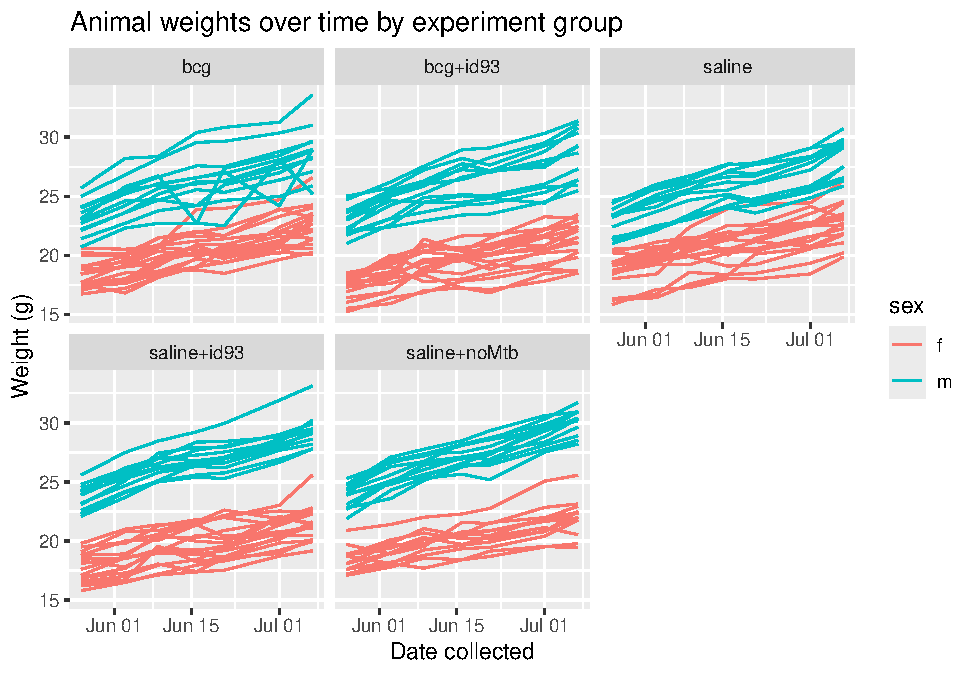
\includegraphics{csu-impactb_files/figure-latex/unnamed-chunk-15-1.pdf}

Next, the code creates boxplots that focus on differences in weights at the
latest available timepoint. One boxplot is created for each experimental
group, and the points for individual mice are shown behind the boxplot, to
provide a better idea of the pattern of variation in individual mice. These
points are colored based on sex, to help explore patterns by sex.

\begin{Shaded}
\begin{Highlighting}[]
\CommentTok{\# Plot animal weight boxplots for the latest time point }
\NormalTok{our\_mouse\_weights }\SpecialCharTok{\%\textgreater{}\%} 
  \FunctionTok{filter}\NormalTok{(date\_collected }\SpecialCharTok{==} \FunctionTok{last}\NormalTok{(date\_collected)) }\SpecialCharTok{\%\textgreater{}\%} 
  \FunctionTok{ggplot}\NormalTok{(}\FunctionTok{aes}\NormalTok{(}\AttributeTok{x =}\NormalTok{ group, }\AttributeTok{y =}\NormalTok{ weight)) }\SpecialCharTok{+} 
  \FunctionTok{geom\_beeswarm}\NormalTok{(}\FunctionTok{aes}\NormalTok{(}\AttributeTok{color =}\NormalTok{ sex)) }\SpecialCharTok{+} 
  \FunctionTok{geom\_boxplot}\NormalTok{(}\AttributeTok{fill =} \ConstantTok{NA}\NormalTok{, }\AttributeTok{color =} \StringTok{"dodgerblue"}\NormalTok{) }\SpecialCharTok{+} 
  \FunctionTok{ggtitle}\NormalTok{(}\StringTok{"Animal weights at last collection by experimental group"}\NormalTok{) }\SpecialCharTok{+} 
  \FunctionTok{labs}\NormalTok{(}\AttributeTok{x =} \StringTok{"Experimental group"}\NormalTok{, }
       \AttributeTok{y =} \StringTok{"Weight (g)"}\NormalTok{)}
\end{Highlighting}
\end{Shaded}

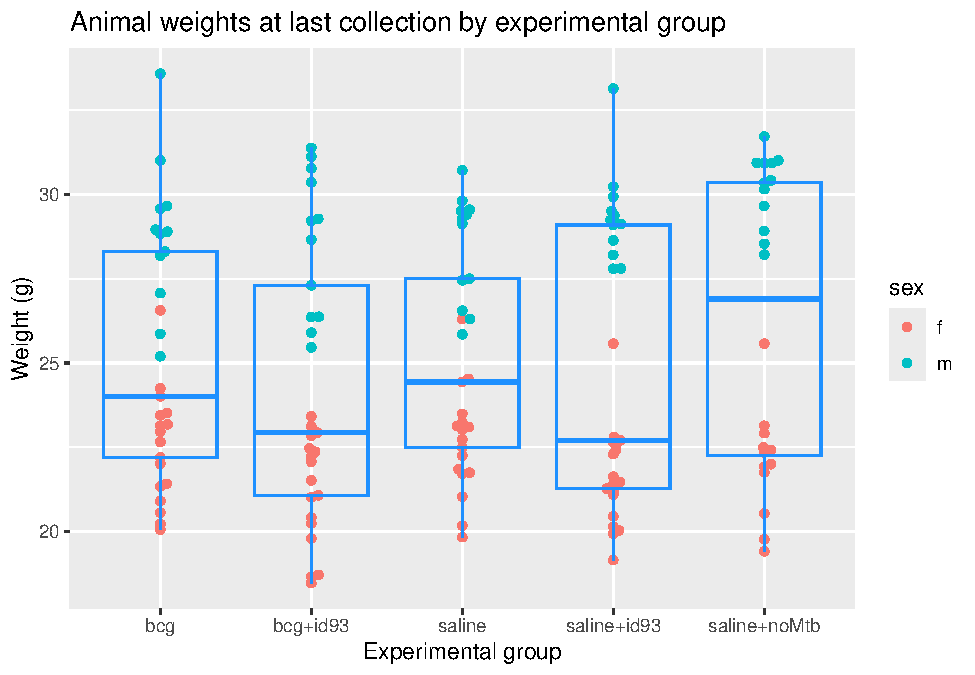
\includegraphics{csu-impactb_files/figure-latex/unnamed-chunk-16-1.pdf}

The next piece of code shows how mouse weights vary by the person who was
handling the animals at a certain time point. Different handlers may have small
differences in how they handle and weight the mice. If there are noticable
differences in the measured weights, this is something that could be corrected
through statisical modeling in later analysis, so we included it as a potential
check.

\begin{Shaded}
\begin{Highlighting}[]
\CommentTok{\# Plot animal weights by animal handler}
\NormalTok{our\_mouse\_weights }\SpecialCharTok{\%\textgreater{}\%} 
  \FunctionTok{ggplot}\NormalTok{(}\FunctionTok{aes}\NormalTok{(}\AttributeTok{x =}\NormalTok{ date\_collected, }\AttributeTok{y =}\NormalTok{ weight, }\AttributeTok{color =}\NormalTok{ who\_collected)) }\SpecialCharTok{+} 
  \FunctionTok{geom\_point}\NormalTok{() }\SpecialCharTok{+} 
  \FunctionTok{ggtitle}\NormalTok{(}\StringTok{"Animal weights by animal handler"}\NormalTok{) }\SpecialCharTok{+} 
  \FunctionTok{labs}\NormalTok{(}\AttributeTok{x =} \StringTok{"Date collected"}\NormalTok{, }
       \AttributeTok{y =} \StringTok{"Weight (g)"}\NormalTok{,}
       \AttributeTok{color =} \StringTok{"Person who}\SpecialCharTok{\textbackslash{}n}\StringTok{handled the}\SpecialCharTok{\textbackslash{}n}\StringTok{animal"}\NormalTok{)}
\end{Highlighting}
\end{Shaded}

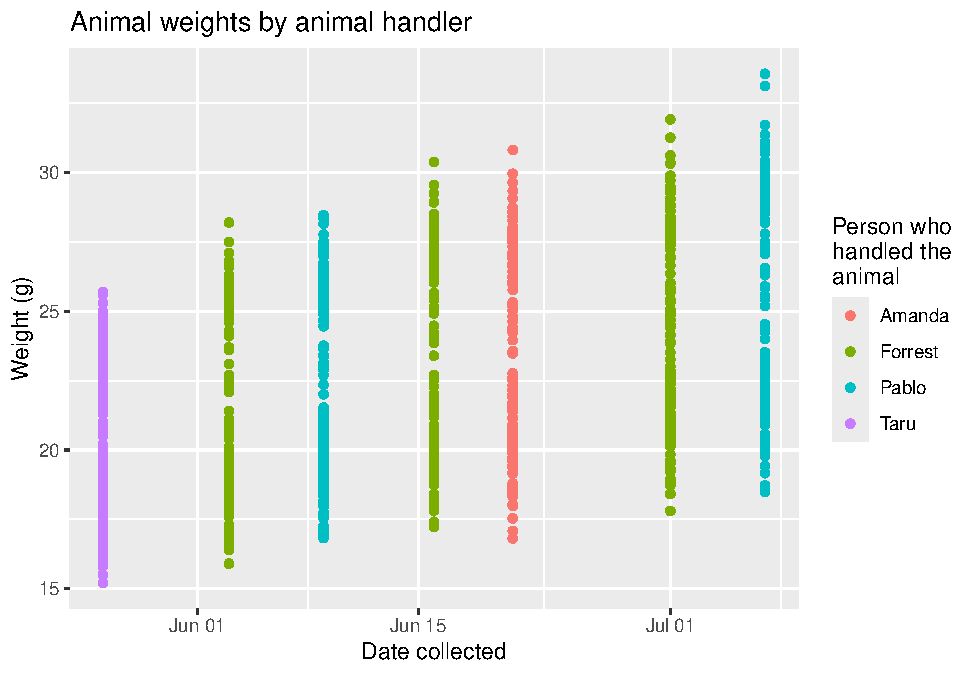
\includegraphics{csu-impactb_files/figure-latex/unnamed-chunk-17-1.pdf}

The next piece of code creates a table with each of the animals that was still
tracked at the last time point (if animals were sacrificed prior to the last
recorded time point, they would not be included here). This table focuses on the
weight change since the previous measured time point. It is ordered by the
change in weight, from the largest decrease to the largest increase. It is meant
as an aide in identifying mice that are showing signs of suffering and may need
to be considered for being euthanized. The animals are labeled in this table by
their most recent cage location, so it will be easier to find them if necessary.
For this example code, we've shown only a sample of 15 animals, but the report
will show data for all animals.

\begin{Shaded}
\begin{Highlighting}[]
\CommentTok{\# Create table of animal weight changes since previous time point}
\NormalTok{our\_mouse\_weights }\SpecialCharTok{\%\textgreater{}\%} 
  \FunctionTok{select}\NormalTok{(date\_collected, weight, group, mouse\_label, sex) }\SpecialCharTok{\%\textgreater{}\%} 
  \FunctionTok{group\_by}\NormalTok{(mouse\_label) }\SpecialCharTok{\%\textgreater{}\%} 
  \FunctionTok{mutate}\NormalTok{(}\AttributeTok{weight\_change =}\NormalTok{ (weight }\SpecialCharTok{{-}} \FunctionTok{lag}\NormalTok{(weight)) }\SpecialCharTok{/} \FunctionTok{lag}\NormalTok{(weight)) }\SpecialCharTok{\%\textgreater{}\%} 
  \FunctionTok{ungroup}\NormalTok{() }\SpecialCharTok{\%\textgreater{}\%} 
  \FunctionTok{filter}\NormalTok{(date\_collected }\SpecialCharTok{==} \FunctionTok{last}\NormalTok{(date\_collected)) }\SpecialCharTok{\%\textgreater{}\%} 
  \FunctionTok{mutate}\NormalTok{(}\AttributeTok{formatted\_weight\_change =} \FunctionTok{paste0}\NormalTok{(}\FunctionTok{formatC}\NormalTok{(weight\_change }\SpecialCharTok{*} \DecValTok{100}\NormalTok{, }
                                                  \AttributeTok{digits =} \DecValTok{1}\NormalTok{, }\AttributeTok{format =} \StringTok{"f"}\NormalTok{), }\StringTok{"\%"}\NormalTok{)) }\SpecialCharTok{\%\textgreater{}\%} 
  \FunctionTok{arrange}\NormalTok{(weight\_change) }\SpecialCharTok{\%\textgreater{}\%} 
  \FunctionTok{select}\NormalTok{(mouse\_label, group, sex, weight, formatted\_weight\_change) }\SpecialCharTok{\%\textgreater{}\%} 
  \FunctionTok{slice}\NormalTok{(}\DecValTok{1}\SpecialCharTok{:}\DecValTok{15}\NormalTok{) }\SpecialCharTok{\%\textgreater{}\%}  \CommentTok{\# Only for the chapter{-}{-}show a sample, not all}
\NormalTok{  knitr}\SpecialCharTok{::}\FunctionTok{kable}\NormalTok{(}\AttributeTok{col.names =} \FunctionTok{c}\NormalTok{(}\StringTok{"Mouse"}\NormalTok{, }\StringTok{"Experimental group"}\NormalTok{, }\StringTok{"Sex"}\NormalTok{, }
                             \StringTok{"Weight (g)"}\NormalTok{, }\StringTok{"Weight change since last measure"}\NormalTok{), }
               \AttributeTok{caption =} \StringTok{"Individual data on weight changes in mice between current measurement and previous measurement."}\NormalTok{)}
\end{Highlighting}
\end{Shaded}

\begin{table}

\caption{\label{tab:unnamed-chunk-18}Individual data on weight changes in mice between current measurement and previous measurement.}
\centering
\begin{tabular}[t]{l|l|l|r|l}
\hline
Mouse & Experimental group & Sex & Weight (g) & Weight change since last measure\\
\hline
Cage: 22021 Notch: 1R & bcg & m & 25.20 & -10.4\%\\
\hline
Cage: 22017 Notch: 1R & saline & f & 23.13 & -4.1\%\\
\hline
Cage: 22015 Notch: 1L & bcg & f & 23.18 & -3.1\%\\
\hline
Cage: 22476 Notch: 1R1L & saline+noMtb & f & 20.54 & -2.8\%\\
\hline
Cage: 22014 Notch: 1L & saline+id93 & f & 21.47 & -2.8\%\\
\hline
Cage: 22014 Notch: 0 & saline+id93 & f & 21.40 & -2.7\%\\
\hline
Cage: 22006 Notch: 1R1L & bcg+id93 & f & 21.02 & -2.4\%\\
\hline
Cage: 22015 Notch: 0 & bcg & f & 20.06 & -1.0\%\\
\hline
Cage: 22004 Notch: 1R & bcg & f & 21.42 & -1.0\%\\
\hline
Cage: 22006 Notch: 0 & bcg+id93 & f & 18.67 & -0.7\%\\
\hline
Cage: 22476 Notch: 0 & saline+noMtb & f & 19.42 & -0.6\%\\
\hline
Cage: 22016 Notch: 1R1L & bcg+id93 & f & 23.13 & -0.5\%\\
\hline
Cage: 22012 Notch: 1R & saline+id93 & f & 22.44 & -0.4\%\\
\hline
Cage: 22015 Notch: 2L & bcg & f & 20.56 & -0.3\%\\
\hline
Cage: 22013B Notch: 1L & saline+id93 & f & 20.46 & -0.2\%\\
\hline
\end{tabular}
\end{table}

As a last step, the code in the template writes a CSV file with the processed
data. This file will be an input into a script that will format the data to
add to a database where we are collecting and integrating data from all the CSU
experiments, and ultimately from there into project-wide storage.

\begin{Shaded}
\begin{Highlighting}[]
\CommentTok{\# Write out processed data into a CSV file}
\FunctionTok{write\_csv}\NormalTok{(our\_mouse\_weights, }\StringTok{"example\_mouse\_output.csv"}\NormalTok{)}
\end{Highlighting}
\end{Shaded}

\hypertarget{colony-forming-units-to-determine-bacterial-counts}{%
\chapter{Colony forming units to determine bacterial counts}\label{colony-forming-units-to-determine-bacterial-counts}}

\hypertarget{downloads-1}{%
\subsection{Downloads}\label{downloads-1}}

The downloads for this chapter are:

\begin{itemize}
\tightlist
\item
  {[}Data collection template{]} for recording colony forming units counted on each
  plate or section of plate in the laboratory
\item
  {[}Report template{]} to process data collected with the data template (when you go to this link, go to the ``File'' bar in your browser's menu bar, chose ``Save As'', then save the file as ``animal\_weights.Rmd'')
\item
  {[}Example output{]} from the report template
\end{itemize}

\hypertarget{overview-2}{%
\subsection{Overview}\label{overview-2}}

In the experiments, we will need to estimate the bacterial load of
\emph{Mycobacterium tuberculosis} in organs---including lungs and spleens---of
animals from experiments. These measurements help us assess how well a vaccine
has worked in comparison to controls.

We will be estimating bacterial load in an animal organ using the plate count
method with serial dilutions. Serial dilutions allow you to create a
highly diluted sample without needing a massive amount of diluent: as you
increase the dilution one step at a time, you can steadily bring the samples
down to lower bacterial loads per volume. This method is common across
laboratories that study tuberculosis drug efficacy as a method for estimating
bacterial load in animal organs \citep{franzblau2012comprehensive} and is a
well-established method across microbiology in general, dating back to Koch in
the late 1800s \citep{wilson1922proportion, ben2014estimation}.

With this method, we homogenize part of the organ, and then create several
increasingly dilute samples. Each dilution is then spread on a plate with a
medium in which \emph{Mycobacterium tuberculosis} can grow and left to grow for
several weeks at a temperature conducive to \emph{Mycobacterium tuberculosis} growth.
The idea is that individual bacteria from the original sample end up randomly
spread across the surface of the plate, and any bacteria that are viable
(able to reproduce) will form a new colony that, after a while, you'll be able
to see \citep{wilson1922proportion, goldman2015practical}. At the end of this
incubation period, you can count the number of these colony-forming units
(CFUs) on each plate.

To count the number of CFUs, you need a ``just right'' dilution (and
we often won't know what this is until after plating) to have a countable
plate. If you have too high of a dilution (i.e., one with very few viable
bacteria), randomness will play a big role in the CFU count, and you'll estimate
the original with more variability, which isn't ideal. If you have too low
of a dilution (i.e., one with lots of viable bacteria), it will be difficult to
identify separate colonies, and they may compete for resources. (The pattern
you see when the dilution is too low (i.e., too concentrated with bacteria) is
called a lawn---colonies merge together).

Once you identify a good dilution for each sample, the CFU count from this
dilution can be used to estimate the bacterial load in the animal's organ. To
translate from diluted concentration to original concentration, you do a
back-calculation, incorporating both the number of colonies counted at that
dilution and how dilute the sample was \citep{ben2014estimation, goldman2015practical}.

\hypertarget{template-description-1}{%
\subsection{Template description}\label{template-description-1}}

The data are collected in a spreadsheet with multiple sheets. The first sheet
(named ``metadata'') is used to record some metadata for the experiment, while the
following sheets are used to record CFUs counts from the plates used for samples
from each organ, with one sheet per organ. For example, if you plated data
from both the lung and spleen, there would be three sheets in the file: one
with the metadata, one with the plate counts for the lung, and one with the
plate counts for the spleen.

The first sheet, which is the metadata sheet is shown below:

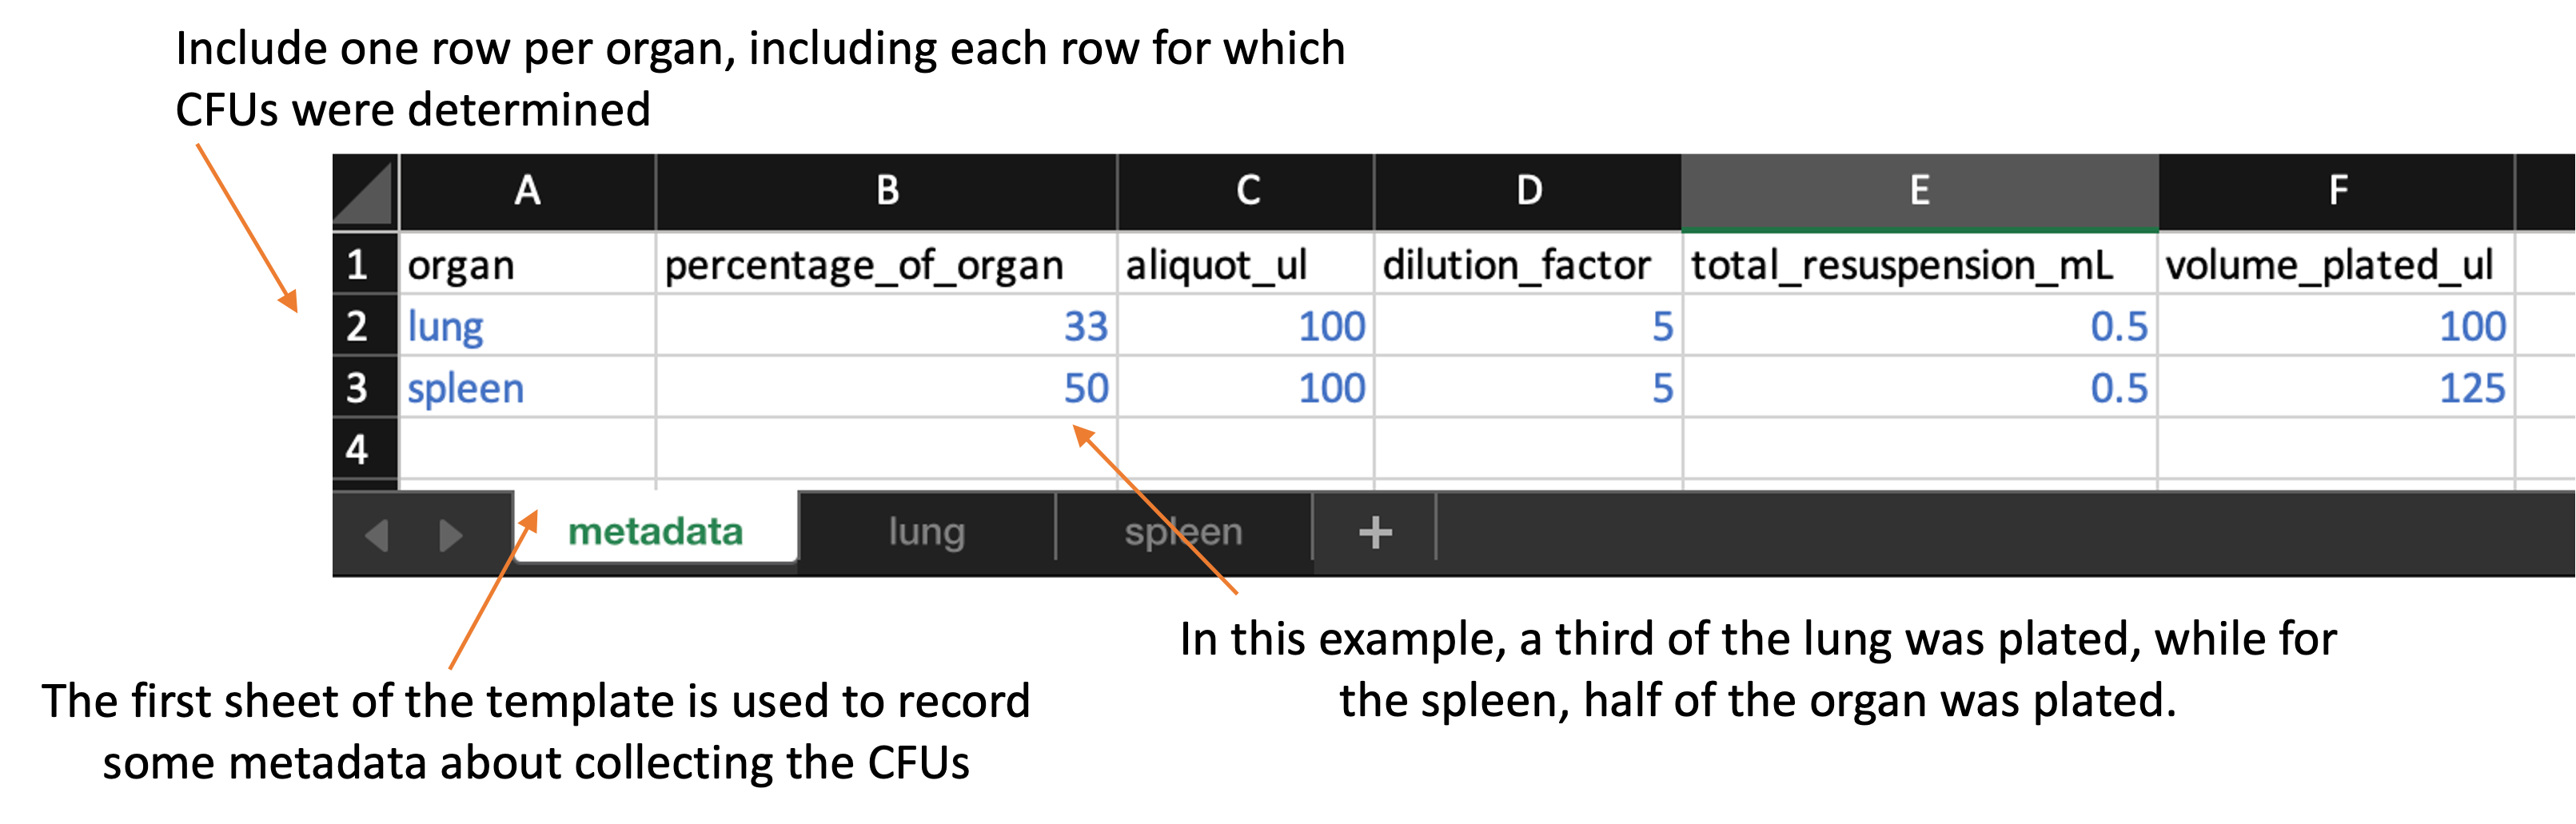
\includegraphics[width=1\linewidth]{figures/cfu_template_metadata}

This metadata sheet is used to record information about the overall process of
plating the data. Values from this sheet will be used in calculating the bacterial
load in the original sample based on the CFU counts. This spreadsheet includes
the following columns:

\begin{itemize}
\tightlist
\item
  \texttt{organ}: Include one row for each organ that was plated in the experiment.
  You should name the organ all in lowercase (e.g., ``lung'', ``spleen''). You
  should use the same name to also name the sheet that records data for that organ
  for example, if you have rows in the metadata sheet for ``lung'' and ``spleen'',
  then you should have two other sheets in the file, one sheet named ``lung'' and
  one named ``spleen'', which you'll use to store the plate counts for each of those
  organs.
\item
  \texttt{percentage\_of\_organ}: In this column, give the proportion of that organ that
  was plated. For example, if you plated half the lung, then in the ``lung'' row
  of this spread sheet, you should put 0.5 in the \texttt{prop\_resuspended} column.
\item
  \texttt{aliquot\_ul}: 100 uL of the total\_resuspended slurry would be considered an original aliquot and is used to peform serial dilutions.
\item
  \texttt{dilution\_factor}: Amount of the original stock solution that is present in the
  total solution, after dilution(s)
\item
  \texttt{total\_resuspended\_mL}: This column contains an original volume of tissue homogenate. For example, raw lung tissue is homogenized in 0.5 mL of PBS in a tube containing metal beads.
\item
  \texttt{volume\_plated\_ul}: Amount of suspension + diluent plated on section of solid agar
\end{itemize}

Following this first sheet in the file, you should have one sheet for each
organ. The organs that you record in these sheets should match up with the rows
on the first, metadata sheet of the template.

Each of these organ-specific sheets should look like this:

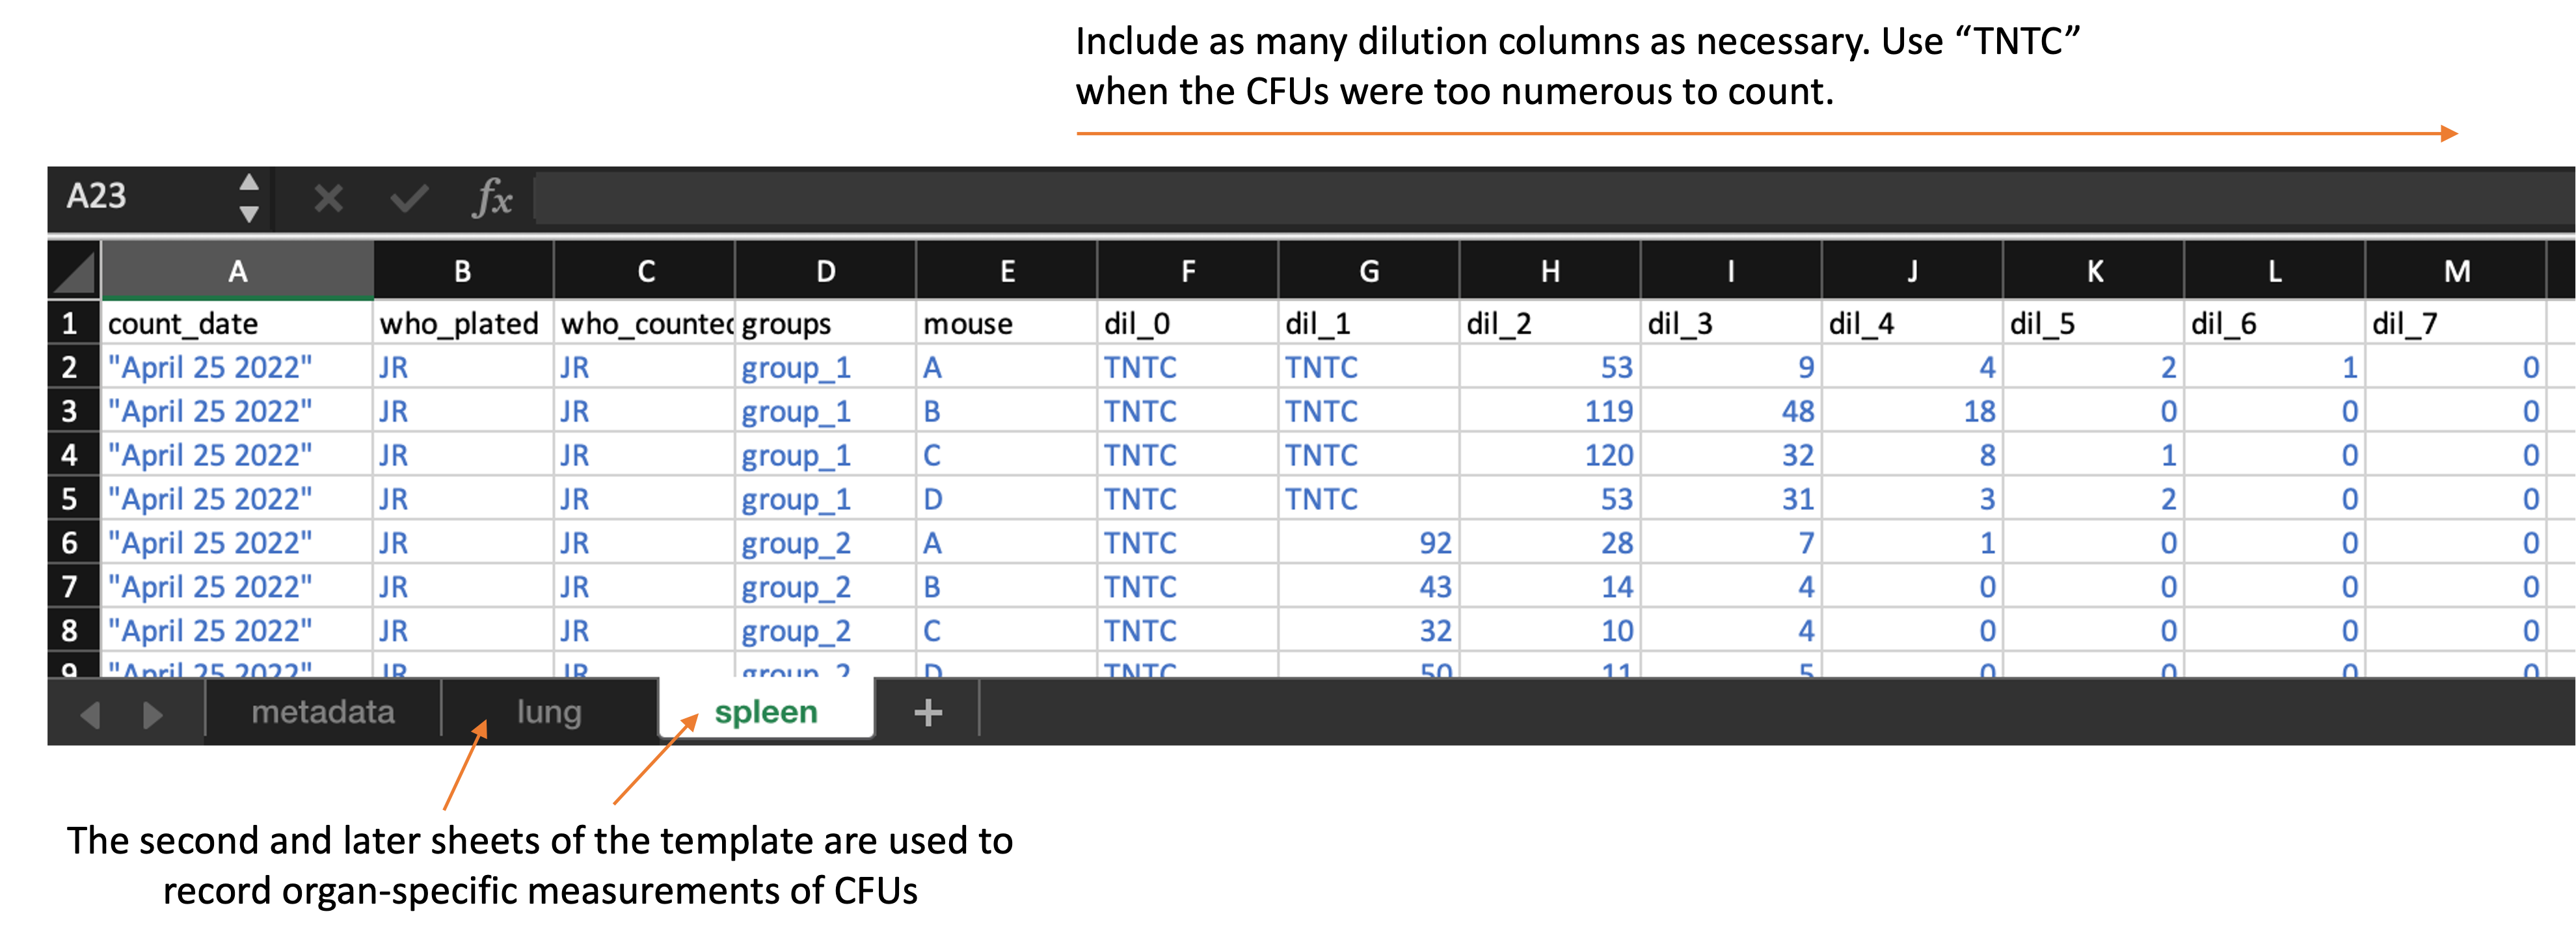
\includegraphics[width=1\linewidth]{figures/cfu_organ_sheet_example}

Each of these organ-specific sheets of the template include the following columns:

\begin{itemize}
\tightlist
\item
  \texttt{count\_date}: The date that the CFUs were counted. In some cases, the same plates
  may be counted at multiple dates.
\item
  \texttt{who\_plated}: An identifier for the researcher who plated the sample
\item
  \texttt{who\_counted}: An identifier for the researcher who counted the plate on this
  specific date
\item
  \texttt{groups}: The experimental group to which the mouse belonged to
\item
  \texttt{mouse}: An identifier for the unique mouse within the group (\emph{note: as we
  collect data from the new experiment, this can be a unique ID by mouse, based on
  notch ID and cage number})
\item
  \texttt{dil\_0}, \texttt{dil\_1}, \texttt{dil\_2}, \ldots: The count at each dilution. You can add additional
  columns if there were more dilutions that are in the template or take away
  dilution columns if there were fewer. However, all dilution columns should be
  named consistently, with ``dil\_'' followed by the dilution number (e.g., ``0'', ``1'',
  ``2''). If the CFUs were too numerous to count for a sample at a particular
  dilution, put ``TNTC'' in that cell of the spreadsheet.
\end{itemize}

When you download the template, it will have example values filled out in blue.
Use these to get an idea for how to record your own data. When you are ready
to record your own data, delete these example values and replace them with
data collected from your own experiment.

\hypertarget{processing-collected-data-1}{%
\subsection{Processing collected data}\label{processing-collected-data-1}}

\hypertarget{details-of-processing-script-1}{%
\subsection{Details of processing script}\label{details-of-processing-script-1}}

\hypertarget{read-in-data}{%
\section{Read in data}\label{read-in-data}}

\begin{Shaded}
\begin{Highlighting}[]
\FunctionTok{library}\NormalTok{(readxl)}
\FunctionTok{library}\NormalTok{(dplyr)}
\FunctionTok{library}\NormalTok{(purrr)}
\FunctionTok{library}\NormalTok{(tidyr)}
\FunctionTok{library}\NormalTok{(stringr)}
\FunctionTok{library}\NormalTok{(tidyverse)}
\FunctionTok{library}\NormalTok{(gridExtra)}
\FunctionTok{library}\NormalTok{(ggplot2)}
\FunctionTok{library}\NormalTok{(ggpubr)}

\CommentTok{\#Replace w/ path to CFU sheet}
\NormalTok{path }\OtherTok{\textless{}{-}} \FunctionTok{c}\NormalTok{(}\StringTok{"DATA/Copy of baa\_cfu\_sheet.xlsx"}\NormalTok{)}

\NormalTok{sheet\_names }\OtherTok{\textless{}{-}} \FunctionTok{excel\_sheets}\NormalTok{(path)}
\NormalTok{sheet\_names }\OtherTok{\textless{}{-}}\NormalTok{ sheet\_names[}\SpecialCharTok{!}\NormalTok{sheet\_names }\SpecialCharTok{\%in\%} \FunctionTok{c}\NormalTok{(}\StringTok{"metadata"}\NormalTok{)]}

\NormalTok{merged\_data }\OtherTok{\textless{}{-}} \FunctionTok{list}\NormalTok{()}

\ControlFlowTok{for}\NormalTok{(i }\ControlFlowTok{in} \DecValTok{1}\SpecialCharTok{:}\FunctionTok{length}\NormalTok{(sheet\_names))\{}
  
\NormalTok{  data }\OtherTok{\textless{}{-}} \FunctionTok{read\_excel}\NormalTok{(path, }\AttributeTok{sheet =}\NormalTok{ sheet\_names[i]) }\SpecialCharTok{\%\textgreater{}\%} 
    \FunctionTok{mutate}\NormalTok{(}\AttributeTok{organ =} \FunctionTok{paste0}\NormalTok{(sheet\_names[i]))}
  
\NormalTok{  data }\OtherTok{\textless{}{-}}\NormalTok{ data }\SpecialCharTok{\%\textgreater{}\%} 
    \CommentTok{\#mutate(missing\_col = NA) \%\textgreater{}\% }
    \FunctionTok{mutate\_if}\NormalTok{(is.double, as.numeric) }\SpecialCharTok{\%\textgreater{}\%} 
    \FunctionTok{mutate\_if}\NormalTok{(is.numeric, as.character) }\SpecialCharTok{\%\textgreater{}\%} 
    \FunctionTok{pivot\_longer}\NormalTok{(}\FunctionTok{starts\_with}\NormalTok{(}\StringTok{"dil\_"}\NormalTok{), }\AttributeTok{names\_to =} \StringTok{"dilution"}\NormalTok{,}
                 \AttributeTok{values\_to =} \StringTok{"CFUs"}\NormalTok{) }\SpecialCharTok{\%\textgreater{}\%} 
    \FunctionTok{mutate}\NormalTok{(}\AttributeTok{dilution =} \FunctionTok{str\_extract}\NormalTok{(dilution, }\StringTok{"[0{-}9]+"}\NormalTok{),}
           \AttributeTok{dilution =} \FunctionTok{as.numeric}\NormalTok{(dilution))}
    
  
\NormalTok{  merged\_data[[i]] }\OtherTok{\textless{}{-}}\NormalTok{ data}
  
  
\NormalTok{\}}
  
\NormalTok{all\_data }\OtherTok{\textless{}{-}} \FunctionTok{bind\_rows}\NormalTok{(merged\_data, }\AttributeTok{.id =} \StringTok{"column\_label"}\NormalTok{) }\SpecialCharTok{\%\textgreater{}\%} 
    \FunctionTok{select}\NormalTok{(}\SpecialCharTok{{-}}\NormalTok{column\_label)}
  
\FunctionTok{head}\NormalTok{(merged\_data)}
\end{Highlighting}
\end{Shaded}

\begin{verbatim}
## [[1]]
## # A tibble: 342 x 8
##    count_date           who_plated who_counted groups mouse organ dilution CFUs 
##    <chr>                <chr>      <chr>       <chr>  <chr> <chr>    <dbl> <chr>
##  1 "\"February 21 2022~ BK         BK          group~ A     lung         0 TNTC 
##  2 "\"February 21 2022~ BK         BK          group~ A     lung         1 TNTC 
##  3 "\"February 21 2022~ BK         BK          group~ A     lung         2 TNTC 
##  4 "\"February 21 2022~ BK         BK          group~ A     lung         3 53   
##  5 "\"February 21 2022~ BK         BK          group~ A     lung         4 9    
##  6 "\"February 21 2022~ BK         BK          group~ A     lung         5 4    
##  7 "\"February 21 2022~ BK         BK          group~ A     lung         6 2    
##  8 "\"February 21 2022~ BK         BK          group~ A     lung         7 1    
##  9 "\"February 21 2022~ BK         BK          group~ A     lung         8 0    
## 10 "\"February 21 2022~ BK         BK          group~ B     lung         0 TNTC 
## # ... with 332 more rows
## 
## [[2]]
## # A tibble: 112 x 8
##    count_date          who_plated who_counted groups  mouse organ dilution CFUs 
##    <chr>               <chr>      <chr>       <chr>   <chr> <chr>    <dbl> <chr>
##  1 "\"April 25 2022\"" JR         JR          group_1 A     sple~        0 TNTC 
##  2 "\"April 25 2022\"" JR         JR          group_1 A     sple~        1 TNTC 
##  3 "\"April 25 2022\"" JR         JR          group_1 A     sple~        2 53   
##  4 "\"April 25 2022\"" JR         JR          group_1 A     sple~        3 9    
##  5 "\"April 25 2022\"" JR         JR          group_1 A     sple~        4 4    
##  6 "\"April 25 2022\"" JR         JR          group_1 A     sple~        5 2    
##  7 "\"April 25 2022\"" JR         JR          group_1 A     sple~        6 1    
##  8 "\"April 25 2022\"" JR         JR          group_1 A     sple~        7 0    
##  9 "\"April 25 2022\"" JR         JR          group_1 B     sple~        0 TNTC 
## 10 "\"April 25 2022\"" JR         JR          group_1 B     sple~        1 TNTC 
## # ... with 102 more rows
\end{verbatim}

\begin{Shaded}
\begin{Highlighting}[]
\FunctionTok{head}\NormalTok{(all\_data)}
\end{Highlighting}
\end{Shaded}

\begin{verbatim}
## # A tibble: 6 x 8
##   count_date            who_plated who_counted groups mouse organ dilution CFUs 
##   <chr>                 <chr>      <chr>       <chr>  <chr> <chr>    <dbl> <chr>
## 1 "\"February 21 2022\~ BK         BK          group~ A     lung         0 TNTC 
## 2 "\"February 21 2022\~ BK         BK          group~ A     lung         1 TNTC 
## 3 "\"February 21 2022\~ BK         BK          group~ A     lung         2 TNTC 
## 4 "\"February 21 2022\~ BK         BK          group~ A     lung         3 53   
## 5 "\"February 21 2022\~ BK         BK          group~ A     lung         4 9    
## 6 "\"February 21 2022\~ BK         BK          group~ A     lung         5 4
\end{verbatim}

\hypertarget{example-one}{%
\section{Example one}\label{example-one}}

\hypertarget{exploratory-analysis-and-quality-checks}{%
\section{Exploratory analysis and quality checks}\label{exploratory-analysis-and-quality-checks}}

\hypertarget{exploratory-analysis}{%
\section{Exploratory analysis}\label{exploratory-analysis}}

\textbf{Dimensions of input data:}

Based on the input data, data were collected for the following organ or
organs:

The following number of mice were included for each:

The following number of replicates were recorded at each count date for
each experimental group:

The following number of dilutions and dilution level were recorded for
each organ:

\textbf{People who plated and collected the data. Date or dates of counting:}

Based on the input data, the plates included in these data were counted by
the following person or persons:
Based on the input data, the plates included in these data were counted on
the following date or dates:

\begin{Shaded}
\begin{Highlighting}[]
\NormalTok{all\_data }\SpecialCharTok{\%\textgreater{}\%}
  \FunctionTok{select}\NormalTok{(organ, who\_plated, who\_counted, count\_date) }\SpecialCharTok{\%\textgreater{}\%}
  \FunctionTok{distinct}\NormalTok{()}
\end{Highlighting}
\end{Shaded}

\begin{verbatim}
## # A tibble: 3 x 4
##   organ  who_plated who_counted count_date            
##   <chr>  <chr>      <chr>       <chr>                 
## 1 lung   BK         BK          "\"February 21 2022\""
## 2 lung   BK         BK          "\"April 18 2022\""   
## 3 spleen JR         JR          "\"April 25 2022\""
\end{verbatim}

\begin{Shaded}
\begin{Highlighting}[]
\FunctionTok{head}\NormalTok{(all\_data)}
\end{Highlighting}
\end{Shaded}

\begin{verbatim}
## # A tibble: 6 x 8
##   count_date            who_plated who_counted groups mouse organ dilution CFUs 
##   <chr>                 <chr>      <chr>       <chr>  <chr> <chr>    <dbl> <chr>
## 1 "\"February 21 2022\~ BK         BK          group~ A     lung         0 TNTC 
## 2 "\"February 21 2022\~ BK         BK          group~ A     lung         1 TNTC 
## 3 "\"February 21 2022\~ BK         BK          group~ A     lung         2 TNTC 
## 4 "\"February 21 2022\~ BK         BK          group~ A     lung         3 53   
## 5 "\"February 21 2022\~ BK         BK          group~ A     lung         4 9    
## 6 "\"February 21 2022\~ BK         BK          group~ A     lung         5 4
\end{verbatim}

\textbf{Distribution of CFUs at each dilution:}

Here's a plot that shows how many plates were too numerous to count at each
dilution level:

Here is a plot that shows how the CFU counts were distributed by dilution
level in the data:

\hypertarget{identify-a-good-dilution-for-each-sample}{%
\section{Identify a good dilution for each sample}\label{identify-a-good-dilution-for-each-sample}}

\begin{Shaded}
\begin{Highlighting}[]
\CommentTok{\# Make all\_data into tidy data and filter for CFUs between 10{-}75}
  
\NormalTok{tidy\_cfu\_data }\OtherTok{\textless{}{-}}\NormalTok{ all\_data }\SpecialCharTok{\%\textgreater{}\%}
  \FunctionTok{mutate}\NormalTok{(}\AttributeTok{dilution =} \FunctionTok{str\_extract}\NormalTok{(dilution, }\StringTok{"[0{-}9]+"}\NormalTok{),}
         \AttributeTok{dilution =} \FunctionTok{as.numeric}\NormalTok{(dilution)) }\SpecialCharTok{\%\textgreater{}\%}
  \FunctionTok{filter}\NormalTok{((CFUs }\SpecialCharTok{\textgreater{}=} \DecValTok{5} \SpecialCharTok{\&}\NormalTok{ CFUs }\SpecialCharTok{\textless{}=} \DecValTok{95}\NormalTok{) }\SpecialCharTok{|}\NormalTok{ groups }\SpecialCharTok{==} \StringTok{"control"}\NormalTok{) }\SpecialCharTok{\%\textgreater{}\%}
  \FunctionTok{mutate}\NormalTok{(}\AttributeTok{CFUs =} \FunctionTok{as.numeric}\NormalTok{(CFUs)) }


\FunctionTok{head}\NormalTok{(tidy\_cfu\_data)}
\end{Highlighting}
\end{Shaded}

\begin{verbatim}
## # A tibble: 6 x 8
##   count_date            who_plated who_counted groups mouse organ dilution  CFUs
##   <chr>                 <chr>      <chr>       <chr>  <chr> <chr>    <dbl> <dbl>
## 1 "\"February 21 2022\~ BK         BK          group~ A     lung         3    53
## 2 "\"February 21 2022\~ BK         BK          group~ A     lung         4     9
## 3 "\"February 21 2022\~ BK         BK          group~ C     lung         5     8
## 4 "\"February 21 2022\~ BK         BK          group~ D     lung         3    53
## 5 "\"February 21 2022\~ BK         BK          group~ A     lung         2    92
## 6 "\"February 21 2022\~ BK         BK          group~ A     lung         4     7
\end{verbatim}

\hypertarget{calculate-cfus-from-best-dilutionestimate-bacterial-load-for-each-sample-based-on-good-dilution}{%
\section{Calculate CFUs from best dilution/Estimate bacterial load for each sample based on good dilution}\label{calculate-cfus-from-best-dilutionestimate-bacterial-load-for-each-sample-based-on-good-dilution}}

\begin{Shaded}
\begin{Highlighting}[]
\CommentTok{\# Calculating CFU/ml for every qualifying replicate between 10{-}75 CFUs. Column binding by organ name to the metadata sheet via inner\_join().}
\NormalTok{meta }\OtherTok{\textless{}{-}} \FunctionTok{read\_excel}\NormalTok{(path, }\AttributeTok{sheet =} \StringTok{"metadata"}\NormalTok{)}

\NormalTok{tidy\_cfu\_meta\_joined }\OtherTok{\textless{}{-}} \FunctionTok{inner\_join}\NormalTok{(meta, tidy\_cfu\_data) }\SpecialCharTok{\%\textgreater{}\%}
  \FunctionTok{group\_by}\NormalTok{(groups) }\SpecialCharTok{\%\textgreater{}\%} 
  \FunctionTok{mutate}\NormalTok{(}\AttributeTok{CFUs\_per\_ml =}\NormalTok{ (CFUs }\SpecialCharTok{*}\NormalTok{ (dilution\_factor}\SpecialCharTok{\^{}}\NormalTok{dilution) }\SpecialCharTok{*} 
\NormalTok{                          (total\_resuspension\_mL}\SpecialCharTok{/}\NormalTok{volume\_plated\_ul) }\SpecialCharTok{*} \DecValTok{1000}\NormalTok{)) }\SpecialCharTok{\%\textgreater{}\%}
  \FunctionTok{select}\NormalTok{(organ, count\_date, who\_plated, who\_counted, groups,  mouse, dilution,  }
\NormalTok{         CFUs, CFUs\_per\_ml) }\SpecialCharTok{\%\textgreater{}\%} 
  \FunctionTok{ungroup}\NormalTok{()}
\end{Highlighting}
\end{Shaded}

\begin{verbatim}
## Joining, by = "organ"
\end{verbatim}

\begin{Shaded}
\begin{Highlighting}[]
\FunctionTok{head}\NormalTok{(tidy\_cfu\_meta\_joined)}
\end{Highlighting}
\end{Shaded}

\begin{verbatim}
## # A tibble: 6 x 9
##   organ count_date            who_plated who_counted groups mouse dilution  CFUs
##   <chr> <chr>                 <chr>      <chr>       <chr>  <chr>    <dbl> <dbl>
## 1 lung  "\"February 21 2022\~ BK         BK          group~ A            3    53
## 2 lung  "\"February 21 2022\~ BK         BK          group~ A            4     9
## 3 lung  "\"February 21 2022\~ BK         BK          group~ C            5     8
## 4 lung  "\"February 21 2022\~ BK         BK          group~ D            3    53
## 5 lung  "\"February 21 2022\~ BK         BK          group~ A            2    92
## 6 lung  "\"February 21 2022\~ BK         BK          group~ A            4     7
## # ... with 1 more variable: CFUs_per_ml <dbl>
\end{verbatim}

\hypertarget{create-initial-report-information-for-these-data}{%
\section{Create initial report information for these data}\label{create-initial-report-information-for-these-data}}

\begin{Shaded}
\begin{Highlighting}[]
\NormalTok{tidy\_lung\_cfu\_plot }\OtherTok{\textless{}{-}}\NormalTok{ tidy\_cfu\_meta\_joined }\SpecialCharTok{\%\textgreater{}\%}
  \FunctionTok{filter}\NormalTok{(organ }\SpecialCharTok{==} \StringTok{"lung"}\NormalTok{) }\SpecialCharTok{\%\textgreater{}\%}
  \FunctionTok{mutate}\NormalTok{(}\AttributeTok{group =} \FunctionTok{fct\_relevel}\NormalTok{(groups, }\StringTok{"group\_1"}\NormalTok{, }\StringTok{"group\_2"}\NormalTok{, }\StringTok{"group\_3"}\NormalTok{, }\StringTok{"group\_4"}\NormalTok{)) }\SpecialCharTok{\%\textgreater{}\%}
  \FunctionTok{ggplot}\NormalTok{(}\FunctionTok{aes}\NormalTok{(}\AttributeTok{x =}\NormalTok{ groups, }\AttributeTok{y =} \FunctionTok{log10}\NormalTok{(CFUs\_per\_ml), }\AttributeTok{fill =}\NormalTok{ groups))}\SpecialCharTok{+}
  \FunctionTok{stat\_boxplot}\NormalTok{( }\FunctionTok{aes}\NormalTok{(}\AttributeTok{x =}\NormalTok{ groups, }\AttributeTok{y =} \FunctionTok{log10}\NormalTok{(CFUs\_per\_ml)), }
    \AttributeTok{geom=}\StringTok{\textquotesingle{}errorbar\textquotesingle{}}\NormalTok{, }\AttributeTok{linetype=}\DecValTok{1}\NormalTok{, }\AttributeTok{width=}\FloatTok{0.5}\NormalTok{)}\SpecialCharTok{+} 
  \FunctionTok{geom\_boxplot}\NormalTok{(}\FunctionTok{aes}\NormalTok{(}\AttributeTok{group =}\NormalTok{ groups), }\AttributeTok{fill =} \ConstantTok{NA}\NormalTok{, }\AttributeTok{show.legend =} \ConstantTok{FALSE}\NormalTok{, }\AttributeTok{color =} \StringTok{"lightgrey"}\NormalTok{)}\SpecialCharTok{+}
  \FunctionTok{geom\_point}\NormalTok{(}\AttributeTok{show.legend =} \ConstantTok{FALSE}\NormalTok{)}\SpecialCharTok{+}
  \FunctionTok{labs}\NormalTok{(}\AttributeTok{title =} \FunctionTok{paste0}\NormalTok{(}\StringTok{"CFUs in early infected mouse lung"}\NormalTok{), }\AttributeTok{x =} \StringTok{"Group"}\NormalTok{, }\AttributeTok{y =} \StringTok{"log10(CFU/mL)"}\NormalTok{,}
       \AttributeTok{color =} \StringTok{"Group"}\NormalTok{)}\SpecialCharTok{+}
  \FunctionTok{guides}\NormalTok{(}\AttributeTok{shape =} \StringTok{"none"}\NormalTok{)}\SpecialCharTok{+}
  \FunctionTok{theme\_minimal}\NormalTok{()}\SpecialCharTok{+}
  \FunctionTok{stat\_compare\_means}\NormalTok{(}\AttributeTok{label =} \StringTok{"p.signif"}\NormalTok{, }\AttributeTok{method =} \StringTok{"t.test"}\NormalTok{, }\AttributeTok{ref.group =} \StringTok{"group\_1"}\NormalTok{) }\SpecialCharTok{+} 
  \FunctionTok{scale\_y\_continuous}\NormalTok{(}\AttributeTok{expand =} \FunctionTok{c}\NormalTok{(}\DecValTok{0}\NormalTok{, }\DecValTok{0}\NormalTok{), }\AttributeTok{limits =} \FunctionTok{c}\NormalTok{(}\DecValTok{0}\NormalTok{, }\DecValTok{8}\NormalTok{))}

\NormalTok{tidy\_lung\_cfu\_plot}
\end{Highlighting}
\end{Shaded}

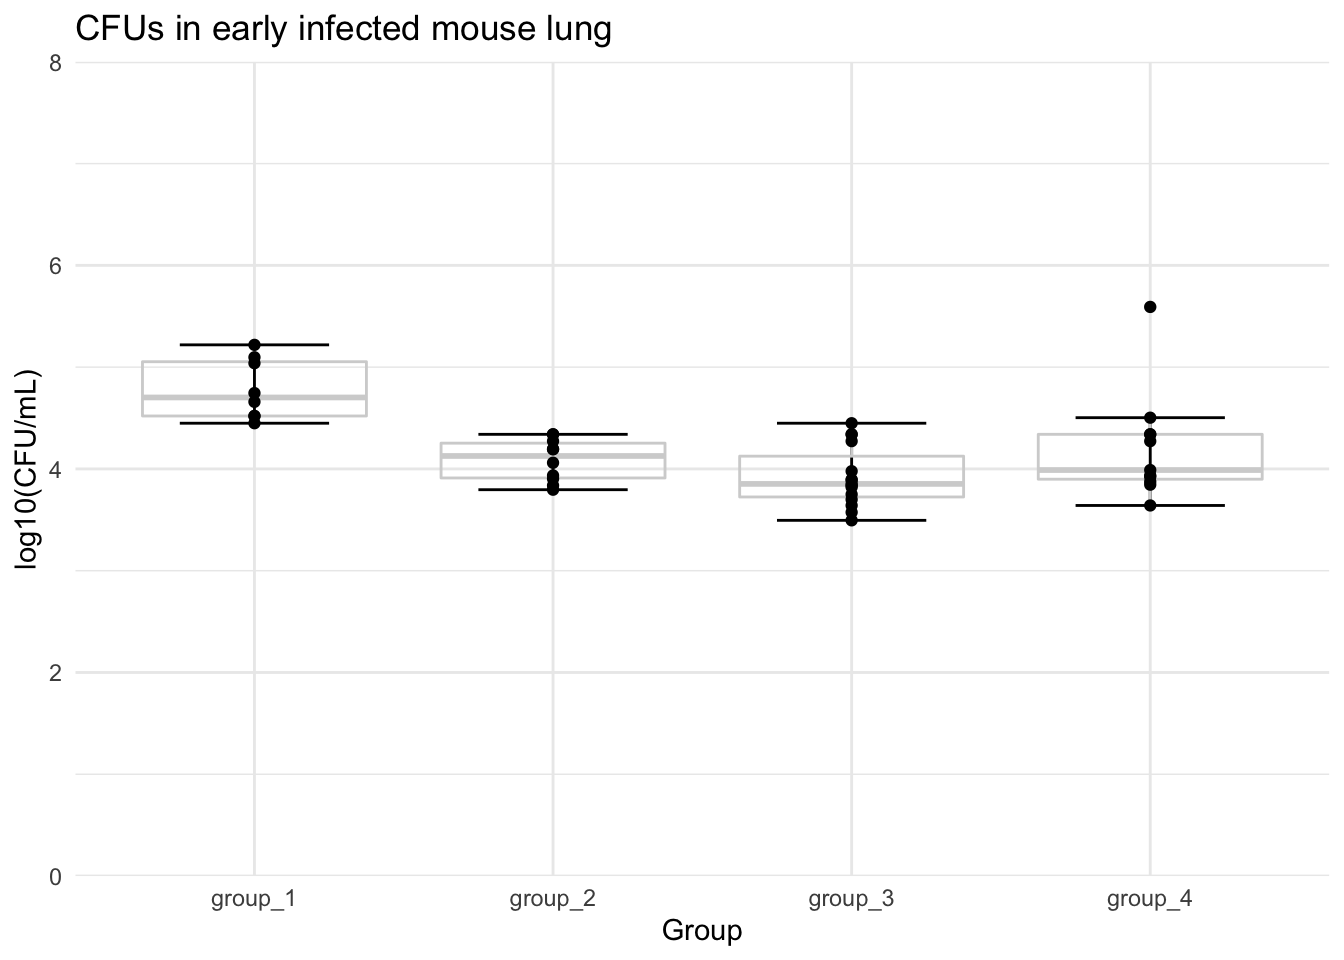
\includegraphics{csu-impactb_files/figure-latex/unnamed-chunk-26-1.pdf}

\hypertarget{sample-anova}{%
\section{Sample ANOVA}\label{sample-anova}}

\begin{Shaded}
\begin{Highlighting}[]
\NormalTok{cfu\_stats }\OtherTok{\textless{}{-}}\NormalTok{ tidy\_cfu\_meta\_joined }\SpecialCharTok{\%\textgreater{}\%} 
  \FunctionTok{group\_by}\NormalTok{(organ) }\SpecialCharTok{\%\textgreater{}\%}
  \FunctionTok{nest}\NormalTok{() }\SpecialCharTok{\%\textgreater{}\%}
  \FunctionTok{mutate}\NormalTok{(}\AttributeTok{aov\_result =} \FunctionTok{map}\NormalTok{(data, }\SpecialCharTok{\textasciitilde{}}\FunctionTok{aov}\NormalTok{(CFUs\_per\_ml }\SpecialCharTok{\textasciitilde{}}\NormalTok{ groups, }\AttributeTok{data =}\NormalTok{ .x)),}
         \AttributeTok{tukey\_result =} \FunctionTok{map}\NormalTok{(aov\_result, TukeyHSD),}
         \AttributeTok{tidy\_tukey =} \FunctionTok{map}\NormalTok{(tukey\_result, broom}\SpecialCharTok{::}\NormalTok{tidy)) }\SpecialCharTok{\%\textgreater{}\%}
  \FunctionTok{unnest}\NormalTok{(tidy\_tukey, }\AttributeTok{.drop =} \ConstantTok{TRUE}\NormalTok{) }\SpecialCharTok{\%\textgreater{}\%}
  \FunctionTok{separate}\NormalTok{(contrast, }\AttributeTok{into =} \FunctionTok{c}\NormalTok{(}\StringTok{"contrast1"}\NormalTok{, }\StringTok{"contrast2"}\NormalTok{), }\AttributeTok{sep =} \StringTok{"{-}"}\NormalTok{) }\SpecialCharTok{\%\textgreater{}\%}
  \FunctionTok{select}\NormalTok{(}\SpecialCharTok{{-}}\NormalTok{data, }\SpecialCharTok{{-}}\NormalTok{aov\_result, }\SpecialCharTok{{-}}\NormalTok{tukey\_result, }\SpecialCharTok{{-}}\NormalTok{term, }\SpecialCharTok{{-}}\NormalTok{null.value)}\CommentTok{\# \%\textgreater{}\%}
\end{Highlighting}
\end{Shaded}

\begin{verbatim}
## Warning: The `.drop` argument of `unnest()` is deprecated as of tidyr 1.0.0.
## All list-columns are now preserved.
## This warning is displayed once every 8 hours.
## Call `lifecycle::last_lifecycle_warnings()` to see where this warning was generated.
\end{verbatim}

\begin{Shaded}
\begin{Highlighting}[]
  \CommentTok{\# filter(adj.p.value \textless{}= 0.05)}

\NormalTok{cfu\_stats}
\end{Highlighting}
\end{Shaded}

\begin{verbatim}
## # A tibble: 9 x 7
## # Groups:   organ [2]
##   organ  contrast1 contrast2 estimate conf.low conf.high adj.p.value
##   <chr>  <chr>     <chr>        <dbl>    <dbl>     <dbl>       <dbl>
## 1 lung   group_2   group_1    -60953. -138742.    16836.      0.171 
## 2 lung   group_3   group_1    -63903. -135699.     7893.      0.0963
## 3 lung   group_4   group_1    -26214. -102416.    49987.      0.793 
## 4 lung   group_3   group_2     -2950.  -69900.    64000.      0.999 
## 5 lung   group_4   group_2     34739.  -36915.   106393.      0.569 
## 6 lung   group_4   group_3     37689.  -27410.   102787.      0.417 
## 7 spleen group_2   group_1     -6565   -13529.      399.      0.0656
## 8 spleen group_3   group_1     -7310   -13341.    -1279.      0.0178
## 9 spleen group_3   group_2      -745.   -6776.     5286.      0.943
\end{verbatim}

\hypertarget{save-processed-data-to-database}{%
\section{Save processed data to database}\label{save-processed-data-to-database}}

\hypertarget{example-two}{%
\section{Example two}\label{example-two}}

\hypertarget{enzyme-linked-immunosorbest-assay-elisa}{%
\chapter{Enzyme-linked immunosorbest assay (ELISA)}\label{enzyme-linked-immunosorbest-assay-elisa}}

ELISA is a standard molecular biology assay for detecting and quantifying a
variety of compounds, including peptides, proteins, and antibodies in a sample.
The sample could be serum, plasma, or bronchoalveolar lavage fluid (BALF).

\hypertarget{importance-of-elisa}{%
\section{\texorpdfstring{\textbf{Importance of ELISA}}{Importance of ELISA}}\label{importance-of-elisa}}

An antigen-specific reaction in the host results in the production of antibodies, which are proteins found in the blood. In the event of an infectious disease,
it aids in the detection of antibodies in the body. ELISA is distinguishable from other antibody-assays in that it produces quantifiable findings and separates non-specific from specific interactions by serial binding to solid surfaces,
which is often a polystyrene multi-well plate.

In IMPAc-TB project, it is crucial to evaluate the if the vaccine is eliciting humoral immunity and generating antibodies against vaccine antigen. ELISA will
be used to determine the presence of Immunoglobulin (Ig) IgG, IgA, and IgM in
the serum different time points post-vaccination.

\hypertarget{principle-of-elisa}{%
\subsection{\texorpdfstring{\textbf{Principle of ELISA}}{Principle of ELISA}}\label{principle-of-elisa}}

ELISA is based on the principle of antigen-antibody interaction. An antigen must be immobilized on a solid surface and then complexed with an enzyme-linked antibody in an ELISA. The conjugated enzyme's activity is evaluated by incubating it with a substrate to yield a quantifiable result, which enables detection. There are four basic steps of ELISA:

\textbf{1. Coating multiwell plate with antigen/antibody}: This step depends on what we want to detect the sample. If we need to evaluate the the presence of antibody, the plate will be coated with the antigen, and vice versa. To coat the plate, a fixed concentration of antigen (protein) is added to a 96 well high-binding plate (charged plate). Plate is incubated over night with the antigen at 4 degree celsius (as proteins are temperature sensitive) so that antigens are completely bound to the well.

\textbf{2. Blocking}: It is possible that not each and every site of the well is coated with the targeted antigen, and there could be uncovered areas. It is important to block those empty spaces so that primary antibody (which we will add to the next step) binds to these spaces and give us false positive results. For this, microplate well surface-binding sites are blocked with an unrelated protein or other substance.Most common blocking agents are bovine serum albumin, skim milk, and casein. One of the best blocking agents is to use the serum from the organism in which your secondary (detection antibody) is raised. For example, if the secondary antibody is raised in goat, then we can use goat serum as a blocking agent.

\textbf{3. Probing}: Probing is the step where we add sample containing antibodies that we want to detect. This will be the primary antibody. If the antibodies against the antigen (which we have coated) are present in the sample, it will bind to the antigen with high affinity.

\textbf{4. Washing}: After the incubation of sample containing primary antibody, the wells are washed so that any unbound antibody is washed away. Washing solution contains phosphate buffer saline + 0.05\% tween-20 (a mild detergent). 0.05\% tween-20 washes away all the non-specific interactions as those are not strong, but keeps all the specific interaction as those are strong and cannot be detached with mild detergent.

\textbf{5. Detection}: To detect the presence of antibody-antigen complex, a secondary antibody labelled with an enzyme (usually horseradish peroxidase) is added to the wells, incubated and washed.

\textbf{6. Signal Measurement}: Finally to detect ``if'' and ``how much'' of the antibody is present, a chromogenic substrate (like 3,3',5,5'-Tetramethylbenzidine) is added to the wells, which can be cleaved the the enzyme that is tagged to the secondary antibody. The color compund is formed after the addition of the substrate, which is directly proportional to the amount of antibody present in the sample. The plate is read on a plate reader, where color is converted to numbers.

\begin{figure}
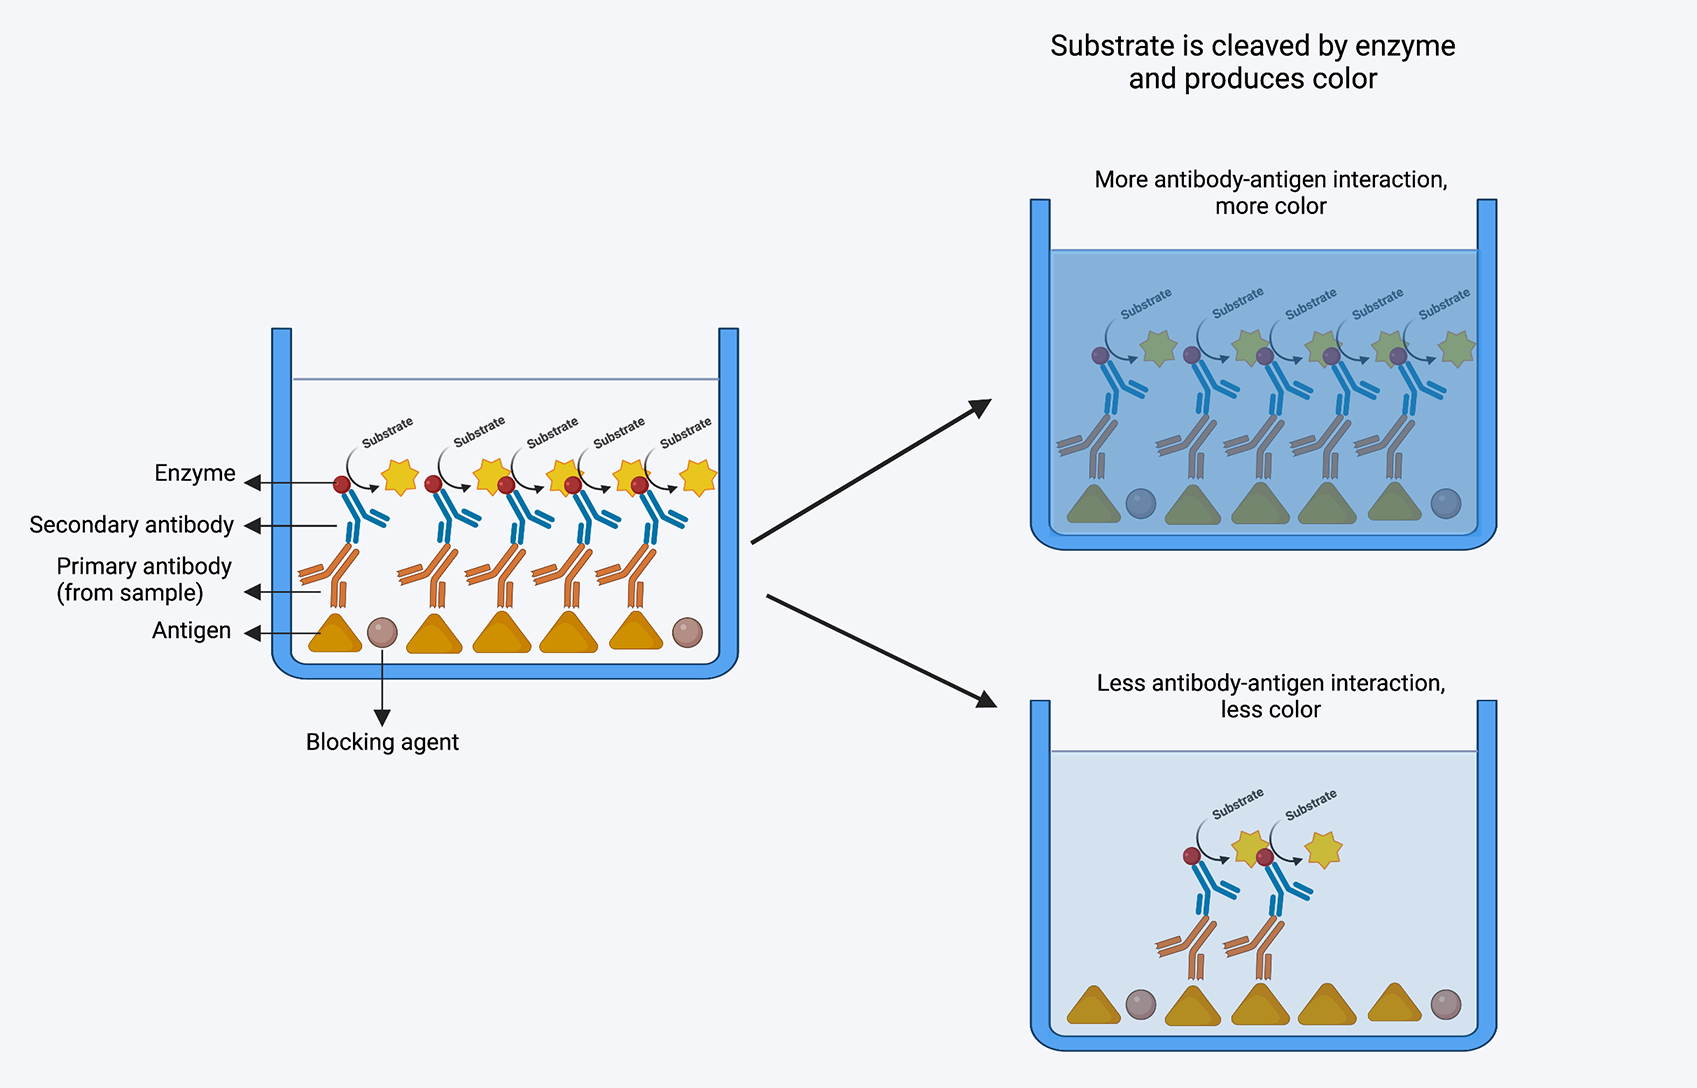
\includegraphics[width=1\linewidth]{DATA/elisa} \caption{A caption}\label{fig:pressure}
\end{figure}

\hypertarget{loading-libraries}{%
\subsection{Loading libraries}\label{loading-libraries}}

\begin{Shaded}
\begin{Highlighting}[]
\FunctionTok{library}\NormalTok{(readxl)}
\FunctionTok{library}\NormalTok{(tidyverse)}
\FunctionTok{library}\NormalTok{(minpack.lm)}
\FunctionTok{library}\NormalTok{(broom)}
\FunctionTok{library}\NormalTok{(purrr)}
\FunctionTok{library}\NormalTok{(ggbeeswarm)}
\end{Highlighting}
\end{Shaded}

\hypertarget{elisa-data-analysis}{%
\section{ELISA data analysis}\label{elisa-data-analysis}}

Analysis of ELISA data is the most important part of the ELISA experiment. ELISA data can be analyzed in different ways based on how the data is acquired. There are a a few examples of the type of ELISA data :

\textbf{1. With standard curve:} ELISA can be used to determine the concentrations of the antigen and antibody. This type of ELISA data usually have a standard curve with
different concentrations of the known analyte and the concentration in the sample is determined by extrapolating the unknown values in the curve. This type of assay is straightforward, easy to interpret and are more robust.

\textbf{2. Without standard curve:} Usually vaccine studies involve investigating the presence of high-affinity (and novel) antibodies against the vaccine antigens.
Therefore, plotting a standard curve is not feasible as there is no previous information available for antibody concentration or type of antibody. Also, because antibody response to a vaccine will differ depending on the individual,
it is not practical to generate a calibration curve from which absolute concentrations can be extrapolated.
For this type of ELISA, quantification of the antibody titers is performed using serial dilutions of the test samples, and analysis can be performed using the following three methods \citep{hartman2018absorbance}:

\begin{enumerate}
\def\labelenumi{\arabic{enumi}.}
\tightlist
\item
  Fitting sigmoid model
\item
  Endpoint titer method
  3: Absorbance summation method
\end{enumerate}

Let's have a look at these methods, how we can apply these methods in our data, and R-based packages that we can utilize to perform this analysis.

\hypertarget{curve-fitting-model}{%
\section{\texorpdfstring{\textbf{1. Curve fitting model:}}{1. Curve fitting model:}}\label{curve-fitting-model}}

The curve in ELISA data represents a plot of known concentrations versus their corresponding signal responses. The typical range of these calibration curves is one to two orders of magnitude on the response axis and two or more orders of magnitude on the concentration axis. The real curve of each assay could be easily identified if an infinite number of concentration dilutions with an infinite number of repetitions could be tested. The correct curve must be approximated from a relatively small number of noisy points, though, because there are a finite number of dilutions that may be performed. To estimate the dose-response relationship between standard dilutions, a method of interpolating between standards is required because there cannot be a standard at every concentration. This process is typically performed using a mathematical function or regression to approximate the true shape of the curve. A curve model is the name given to this approximating function, which commonly uses two or more parameters to describe a family of curves, and are then adjusted in order to find the curve from the family of curves that best fits the assay data.

Three qualities should be included in a good curve fitting model.
1. The true curve's shape must be accurately approximated by the curve model. If the curve model does not accomplish this, there is no way to adjust for this component of the total error that results from a lack of fit.
2. In order to get concentration estimates with minimal inaccuracy, a decent curve model must be able to average away as much of the random variation as is practical. 3. A successful curve model must be capable of accurately predicting concentration values for points between the anchor points of the standard dilutions.

\hypertarget{how-do-we-perform-curve-fitting-model}{%
\subsection{How do we perform curve fitting model}\label{how-do-we-perform-curve-fitting-model}}

There are two major steps in performing curve fitting model for non-linear data like ELISA:
1. Finding the initial starting estimates of the parameters
2. locating the optimal solution in a region of the initial estimates

We have presented an example below where we have performed a 8-10 point serial dilution of our sample and fitted a 4 parameter curve model.

\hypertarget{an-example-of-the-curve-fitting-model}{%
\subsection{An example of the curve fitting model}\label{an-example-of-the-curve-fitting-model}}

\hypertarget{read-in-the-data}{%
\subsubsection{Read in the data}\label{read-in-the-data}}

This information comes from the 2018 study conducted by Hartman et al.~Hartman et al.~analyzed the ELISA data in their study utilizing fitted sigmoid analysis, end point titer, and absorbance summation. We utilized this information to determine whether our formulas and calculations provide the same outcomes and values as theirs.

\begin{Shaded}
\begin{Highlighting}[]
\NormalTok{elisa\_example\_data }\OtherTok{\textless{}{-}} \FunctionTok{read\_excel}\NormalTok{(}\StringTok{"DATA/example\_elisa\_data.xlsx"}\NormalTok{)}
\end{Highlighting}
\end{Shaded}

\hypertarget{tidying-the-data}{%
\subsubsection{Tidying the data}\label{tidying-the-data}}

We next performed tidying the data and make it in a format so that we can plot a sigmoid curve with that.

\begin{Shaded}
\begin{Highlighting}[]
\CommentTok{\# Divide dilution column into two seoparate columns}

\NormalTok{elisa\_example\_data }\OtherTok{\textless{}{-}} \FunctionTok{separate}\NormalTok{(elisa\_example\_data, }
                               \AttributeTok{col =} \StringTok{"dilution"}\NormalTok{, }
                               \AttributeTok{into =} \FunctionTok{c}\NormalTok{(}\StringTok{"numerator"}\NormalTok{, }\StringTok{"denominator"}\NormalTok{), }
                               \AttributeTok{sep =} \StringTok{"}\SpecialCharTok{\textbackslash{}\textbackslash{}}\StringTok{/"}\NormalTok{)}

\CommentTok{\# Convert the tabke from character to numeric}
\NormalTok{elisa\_example\_data }\OtherTok{\textless{}{-}}\NormalTok{ elisa\_example\_data }\SpecialCharTok{\%\textgreater{}\%} 
  \FunctionTok{mutate\_if}\NormalTok{(is.character, as.numeric)}


\NormalTok{elisa\_example\_data}\SpecialCharTok{$}\NormalTok{dilution }\OtherTok{\textless{}{-}} 
\NormalTok{  elisa\_example\_data}\SpecialCharTok{$}\NormalTok{numerator}\SpecialCharTok{/}\NormalTok{elisa\_example\_data}\SpecialCharTok{$}\NormalTok{denominator  }

\NormalTok{elisa\_example\_data }\OtherTok{\textless{}{-}}\NormalTok{ elisa\_example\_data }\SpecialCharTok{\%\textgreater{}\%}
  \FunctionTok{mutate}\NormalTok{(}\AttributeTok{log\_dilution =} \FunctionTok{log}\NormalTok{(dilution, }\AttributeTok{base =} \DecValTok{3}\NormalTok{))}

\FunctionTok{head}\NormalTok{(elisa\_example\_data)}
\end{Highlighting}
\end{Shaded}

\begin{verbatim}
## # A tibble: 6 x 5
##   numerator denominator absorbance dilution log_dilution
##       <dbl>       <dbl>      <dbl>    <dbl>        <dbl>
## 1         1          30       4    0.0333          -3.10
## 2         1          90       3.73 0.0111          -4.10
## 3         1         270       2.34 0.00370         -5.10
## 4         1         810       1.1  0.00123         -6.10
## 5         1        2430       0.51 0.000412        -7.10
## 6         1        7290       0.22 0.000137        -8.10
\end{verbatim}

\hypertarget{create-function-for-curve-fitting-model}{%
\subsubsection{Create function for curve fitting model}\label{create-function-for-curve-fitting-model}}

We next created the curve fitting model function by using nlsLM function from ``minpack.lm'' package.
The purpose of nlslm is to minimize the sum square of the vector returned by the function fn, by a modification of the Levenberg-Marquardt algorithm. In the early 1960s, the Levenberg-Marquardt algorithm was developed to address nonlinear least squares problems. Through a series of well-chosen updates to model parameter values, Levenberg-Marquardt algorithm lower the sum of the squares of the errors between the model function and the data points.

\begin{Shaded}
\begin{Highlighting}[]
\NormalTok{mod\_1 }\OtherTok{\textless{}{-}} \FunctionTok{nlsLM}\NormalTok{(absorbance }\SpecialCharTok{\textasciitilde{}} 
\NormalTok{                 ((a}\SpecialCharTok{{-}}\NormalTok{d)}\SpecialCharTok{/}\NormalTok{(}\DecValTok{1}\SpecialCharTok{+}\NormalTok{(log\_dilution}\SpecialCharTok{/}\NormalTok{c)}\SpecialCharTok{\^{}}\NormalTok{b)) }\SpecialCharTok{+}\NormalTok{ d,}
\AttributeTok{data =}\NormalTok{ elisa\_example\_data, }
\AttributeTok{start =} \FunctionTok{list}\NormalTok{ (}\AttributeTok{a =} \DecValTok{4}\NormalTok{, }\AttributeTok{d=} \DecValTok{0}\NormalTok{, }\AttributeTok{c =} \SpecialCharTok{{-}}\DecValTok{5}\NormalTok{, }\AttributeTok{b =} \DecValTok{1}\NormalTok{))}

\CommentTok{\# a = maximum absorbance}
\CommentTok{\# d = minimum absobance}
\CommentTok{\# c = point of maximum growth }
\CommentTok{\# b = slope at c}

\NormalTok{mod\_1}
\end{Highlighting}
\end{Shaded}

\begin{verbatim}
## Nonlinear regression model
##   model: absorbance ~ ((a - d)/(1 + (log_dilution/c)^b)) + d
##    data: elisa_example_data
##        a        d        c        b 
##  4.12406  0.04532 -5.31056  7.62972 
##  residual sum-of-squares: 0.02221
## 
## Number of iterations to convergence: 9 
## Achieved convergence tolerance: 1.49e-08
\end{verbatim}

\begin{Shaded}
\begin{Highlighting}[]
\FunctionTok{summary}\NormalTok{(mod\_1)}
\end{Highlighting}
\end{Shaded}

\begin{verbatim}
## 
## Formula: absorbance ~ ((a - d)/(1 + (log_dilution/c)^b)) + d
## 
## Parameters:
##   Estimate Std. Error  t value Pr(>|t|)    
## a  4.12406    0.05820   70.860 1.75e-12 ***
## d  0.04532    0.02268    1.998   0.0808 .  
## c -5.31056    0.03933 -135.037 1.01e-14 ***
## b  7.62972    0.35854   21.280 2.50e-08 ***
## ---
## Signif. codes:  0 '***' 0.001 '**' 0.01 '*' 0.05 '.' 0.1 ' ' 1
## 
## Residual standard error: 0.05269 on 8 degrees of freedom
## 
## Number of iterations to convergence: 9 
## Achieved convergence tolerance: 1.49e-08
\end{verbatim}

\hypertarget{apply-the-function-to-the-data}{%
\subsubsection{Apply the function to the data}\label{apply-the-function-to-the-data}}

\begin{Shaded}
\begin{Highlighting}[]
\NormalTok{tidy\_params }\OtherTok{\textless{}{-}}\NormalTok{ mod\_1 }\SpecialCharTok{\%\textgreater{}\%} \FunctionTok{tidy}\NormalTok{() }

\NormalTok{a }\OtherTok{\textless{}{-}}\NormalTok{ tidy\_params}\SpecialCharTok{$}\NormalTok{estimate[tidy\_params}\SpecialCharTok{$}\NormalTok{term }\SpecialCharTok{==} \StringTok{"a"}\NormalTok{]}
\NormalTok{b }\OtherTok{\textless{}{-}}\NormalTok{ tidy\_params}\SpecialCharTok{$}\NormalTok{estimate[tidy\_params}\SpecialCharTok{$}\NormalTok{term }\SpecialCharTok{==} \StringTok{"b"}\NormalTok{]}
\NormalTok{c }\OtherTok{\textless{}{-}}\NormalTok{ tidy\_params}\SpecialCharTok{$}\NormalTok{estimate[tidy\_params}\SpecialCharTok{$}\NormalTok{term }\SpecialCharTok{==} \StringTok{"c"}\NormalTok{]}
\NormalTok{d }\OtherTok{\textless{}{-}}\NormalTok{ tidy\_params}\SpecialCharTok{$}\NormalTok{estimate[tidy\_params}\SpecialCharTok{$}\NormalTok{term }\SpecialCharTok{==} \StringTok{"d"}\NormalTok{]}

\NormalTok{elisa\_example\_data }\OtherTok{\textless{}{-}}\NormalTok{ elisa\_example\_data }\SpecialCharTok{\%\textgreater{}\%}
  \FunctionTok{mutate}\NormalTok{(}\AttributeTok{fitted =} \FunctionTok{predict}\NormalTok{(mod\_1))}

\NormalTok{elisa\_example\_data }\OtherTok{\textless{}{-}}\NormalTok{ elisa\_example\_data }\SpecialCharTok{\%\textgreater{}\%}
  \FunctionTok{mutate}\NormalTok{(}\AttributeTok{fitted =} \FunctionTok{predict}\NormalTok{(mod\_1))}
\end{Highlighting}
\end{Shaded}

\hypertarget{plot-the-sigmoid-curve-with-fitted-sigmoid-model}{%
\subsubsection{Plot the sigmoid curve with fitted sigmoid model}\label{plot-the-sigmoid-curve-with-fitted-sigmoid-model}}

\begin{Shaded}
\begin{Highlighting}[]
\NormalTok{elisa\_example\_data }\SpecialCharTok{\%\textgreater{}\%}
  \FunctionTok{ggplot}\NormalTok{(}\FunctionTok{aes}\NormalTok{(}\AttributeTok{x =}\NormalTok{ log\_dilution, }\AttributeTok{y =}\NormalTok{ absorbance)) }\SpecialCharTok{+}
  \FunctionTok{geom\_point}\NormalTok{() }\SpecialCharTok{+}
  \FunctionTok{geom\_line}\NormalTok{(}\FunctionTok{aes}\NormalTok{(}\AttributeTok{y=}\NormalTok{fitted), }\AttributeTok{color =} \StringTok{"dodgerblue"}\NormalTok{)}
\end{Highlighting}
\end{Shaded}

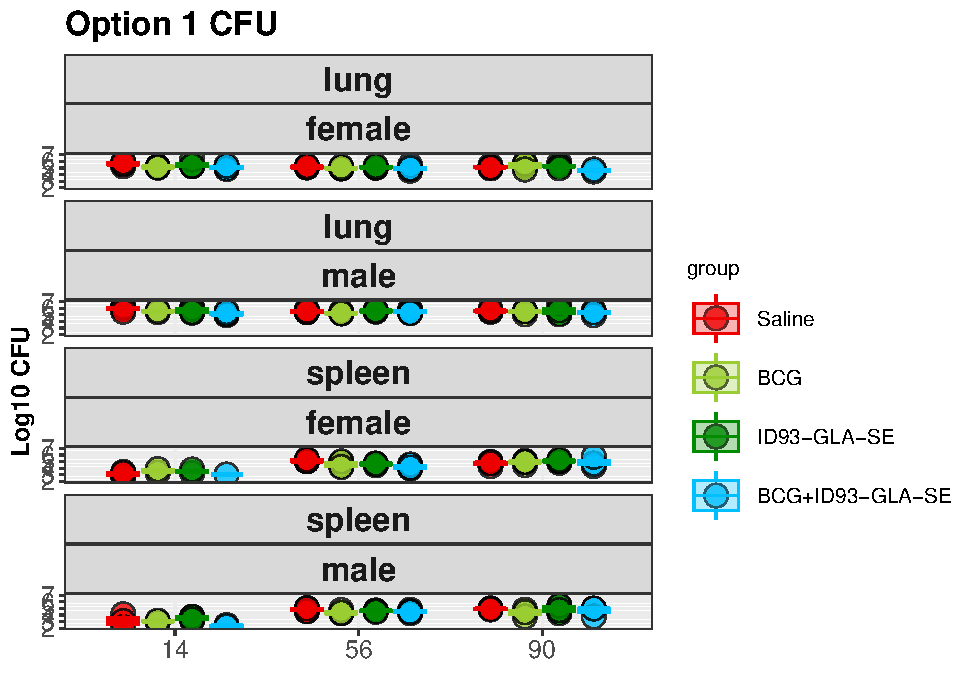
\includegraphics{csu-impactb_files/figure-latex/unnamed-chunk-33-1.pdf}

\hypertarget{endpoint-titer-method}{%
\section{2. Endpoint titer method}\label{endpoint-titer-method}}

The endpoint titer approach chooses an absorbance value just above the background noise (or the lower asymptotic level). \textbf{The highest dilution with an absorbance greater than this predetermined value is the endpoint titer.} This method is based on the assumption that a sample with a higher protein concentration will require a higher dilution factor to achieve an absorbance just above the level of background noise.

\hypertarget{create-an-endpoint-titer-function-and-apply-it-to-the-output-of-the-fitted-sigmoid-model-values.}{%
\subsection{Create an endpoint titer function and apply it to the output of the fitted sigmoid model values.}\label{create-an-endpoint-titer-function-and-apply-it-to-the-output-of-the-fitted-sigmoid-model-values.}}

\begin{Shaded}
\begin{Highlighting}[]
\NormalTok{endpoint\_titer }\OtherTok{\textless{}{-}}\NormalTok{ c }\SpecialCharTok{*}\NormalTok{ (((a }\SpecialCharTok{{-}}\NormalTok{ d) }\SpecialCharTok{/}\NormalTok{ (}\FloatTok{0.2} \SpecialCharTok{{-}}\NormalTok{ d)) }\SpecialCharTok{{-}} \DecValTok{1}\NormalTok{) }\SpecialCharTok{\^{}}\NormalTok{ (}\DecValTok{1} \SpecialCharTok{/}\NormalTok{ b)}

\FunctionTok{summary}\NormalTok{(endpoint\_titer)}
\end{Highlighting}
\end{Shaded}

\begin{verbatim}
##    Min. 1st Qu.  Median    Mean 3rd Qu.    Max. 
##  -8.113  -8.113  -8.113  -8.113  -8.113  -8.113
\end{verbatim}

\begin{Shaded}
\begin{Highlighting}[]
\NormalTok{endpoint\_titer}
\end{Highlighting}
\end{Shaded}

\begin{verbatim}
## [1] -8.113285
\end{verbatim}

\hypertarget{other-methods-to-analyze-elisa-data}{%
\subsection{Other methods to analyze ELISA data}\label{other-methods-to-analyze-elisa-data}}

\hypertarget{absorption-summation}{%
\subsubsection{Absorption summation}\label{absorption-summation}}

\hypertarget{area-under-the-curve}{%
\subsubsection{Area under the curve}\label{area-under-the-curve}}

In this model of data analysis, we sum all the absorbance values from each sample to obtain one value. This value is termed as absorption summation (AS). Using the above data, the AS will be calculated as below:

\begin{Shaded}
\begin{Highlighting}[]
\NormalTok{AS }\OtherTok{=} \FloatTok{0.04} \SpecialCharTok{+} \FloatTok{0.04} \SpecialCharTok{+} \FloatTok{0.05} \SpecialCharTok{+} \FloatTok{0.05} \SpecialCharTok{+} \FloatTok{0.06} \SpecialCharTok{+} 
  \FloatTok{0.1} \SpecialCharTok{+} \FloatTok{0.22} \SpecialCharTok{+} \FloatTok{0.51} \SpecialCharTok{+} \FloatTok{1.1} \SpecialCharTok{+} \FloatTok{2.34} \SpecialCharTok{+} \FloatTok{3.73} \SpecialCharTok{+} \FloatTok{4.0}

\NormalTok{AS}
\end{Highlighting}
\end{Shaded}

\begin{verbatim}
## [1] 12.24
\end{verbatim}

\hypertarget{apply-the-fitting-sigmoid-model-and-endpoint-titer-function-in-our-dataset}{%
\section{Apply the fitting sigmoid model and endpoint titer function in our dataset}\label{apply-the-fitting-sigmoid-model-and-endpoint-titer-function-in-our-dataset}}

The presented data is from a mouse study. In this data, presence of IgG antibody has been evaluated against receptor binding domain (RBD) of SARS-CoV-2 virus in two different groups of mice. We need to elucidate which group has higher concentration of the antibodies.

\hypertarget{read-in-the-data-1}{%
\subsubsection{Read in the data}\label{read-in-the-data-1}}

\begin{Shaded}
\begin{Highlighting}[]
\NormalTok{elisa\_data }\OtherTok{\textless{}{-}} \FunctionTok{read\_excel}\NormalTok{(}\StringTok{"DATA/elisa\_data\_serial\_dilution.xlsx"}\NormalTok{)}
\end{Highlighting}
\end{Shaded}

\hypertarget{tidy-the-data}{%
\subsubsection{Tidy the data}\label{tidy-the-data}}

\begin{Shaded}
\begin{Highlighting}[]
\NormalTok{elisa\_data }\OtherTok{\textless{}{-}} \FunctionTok{pivot\_longer}\NormalTok{(}\AttributeTok{data =}\NormalTok{ elisa\_data, }
                           \AttributeTok{cols =} \StringTok{"Mouse\_1"}\SpecialCharTok{:}\StringTok{"Mouse\_5"}\NormalTok{, }
                           \AttributeTok{names\_to =} \StringTok{"mouse\_id"}\NormalTok{, }
                           \AttributeTok{values\_to =} \StringTok{"absorbance"}\NormalTok{)}

\FunctionTok{head}\NormalTok{(elisa\_data)}
\end{Highlighting}
\end{Shaded}

\begin{verbatim}
## # A tibble: 6 x 4
##   Groups  Dilution mouse_id absorbance
##   <chr>   <chr>    <chr>         <dbl>
## 1 Group 1 1/50     Mouse_1         4.1
## 2 Group 1 1/50     Mouse_2         3.9
## 3 Group 1 1/50     Mouse_3         4.3
## 4 Group 1 1/50     Mouse_4         4.2
## 5 Group 1 1/50     Mouse_5         4  
## 6 Group 1 1/100    Mouse_1         3.9
\end{verbatim}

\begin{Shaded}
\begin{Highlighting}[]
\CommentTok{\# separate dilution column and convert it to log2}

\NormalTok{elisa\_data }\OtherTok{\textless{}{-}} \FunctionTok{separate}\NormalTok{(elisa\_data, }
                       \AttributeTok{col =} \StringTok{"Dilution"}\NormalTok{, }
                       \AttributeTok{into =} \FunctionTok{c}\NormalTok{(}\StringTok{"numerator"}\NormalTok{, }
                                \StringTok{"denomenator"}\NormalTok{), }
                       \AttributeTok{sep =} \StringTok{"}\SpecialCharTok{\textbackslash{}\textbackslash{}}\StringTok{/"}\NormalTok{)}

\NormalTok{elisa\_data }\OtherTok{\textless{}{-}}\NormalTok{ elisa\_data }\SpecialCharTok{\%\textgreater{}\%} 
  \FunctionTok{transform}\NormalTok{(}\AttributeTok{numerator =} \FunctionTok{as.numeric}\NormalTok{(numerator),}
            \AttributeTok{denomenator =} \FunctionTok{as.numeric}\NormalTok{(denomenator))}

\NormalTok{elisa\_data }\OtherTok{\textless{}{-}}\NormalTok{ elisa\_data }\SpecialCharTok{\%\textgreater{}\%}
  \FunctionTok{mutate}\NormalTok{(}\AttributeTok{dilution =} 
\NormalTok{           elisa\_data}\SpecialCharTok{$}\NormalTok{numerator}\SpecialCharTok{/}\NormalTok{elisa\_data}\SpecialCharTok{$}\NormalTok{denomenator) }

\NormalTok{elisa\_data }\OtherTok{\textless{}{-}}\NormalTok{ elisa\_data }\SpecialCharTok{\%\textgreater{}\%}
  \FunctionTok{mutate}\NormalTok{(}\AttributeTok{log\_dilution =} \FunctionTok{log2}\NormalTok{(dilution))}

\FunctionTok{head}\NormalTok{(elisa\_data)}
\end{Highlighting}
\end{Shaded}

\begin{verbatim}
##    Groups numerator denomenator mouse_id absorbance dilution log_dilution
## 1 Group 1         1          50  Mouse_1        4.1     0.02    -5.643856
## 2 Group 1         1          50  Mouse_2        3.9     0.02    -5.643856
## 3 Group 1         1          50  Mouse_3        4.3     0.02    -5.643856
## 4 Group 1         1          50  Mouse_4        4.2     0.02    -5.643856
## 5 Group 1         1          50  Mouse_5        4.0     0.02    -5.643856
## 6 Group 1         1         100  Mouse_1        3.9     0.01    -6.643856
\end{verbatim}

\hypertarget{converting-data-into-dataframe}{%
\paragraph{converting data into dataframe}\label{converting-data-into-dataframe}}

\begin{Shaded}
\begin{Highlighting}[]
\NormalTok{elisa\_data\_df }\OtherTok{\textless{}{-}}\NormalTok{ elisa\_data }\SpecialCharTok{\%\textgreater{}\%} 
  \FunctionTok{group\_by}\NormalTok{(Groups, mouse\_id) }\SpecialCharTok{\%\textgreater{}\%} 
  \FunctionTok{summarize}\NormalTok{(}\AttributeTok{log\_dilution =}\NormalTok{ log\_dilution, }
            \AttributeTok{absorbance =}\NormalTok{ absorbance)}
\end{Highlighting}
\end{Shaded}

\begin{verbatim}
## `summarise()` has grouped output by 'Groups', 'mouse_id'. You can override using
## the `.groups` argument.
\end{verbatim}

\begin{Shaded}
\begin{Highlighting}[]
\NormalTok{elisa\_data\_nested }\OtherTok{\textless{}{-}}\NormalTok{ elisa\_data }\SpecialCharTok{\%\textgreater{}\%}
  \FunctionTok{group\_by}\NormalTok{(Groups, mouse\_id) }\SpecialCharTok{\%\textgreater{}\%}
  \FunctionTok{nest}\NormalTok{()}

\FunctionTok{head}\NormalTok{(elisa\_data\_nested)}
\end{Highlighting}
\end{Shaded}

\begin{verbatim}
## # A tibble: 6 x 3
## # Groups:   Groups, mouse_id [6]
##   Groups  mouse_id data             
##   <chr>   <chr>    <list>           
## 1 Group 1 Mouse_1  <tibble [10 x 5]>
## 2 Group 1 Mouse_2  <tibble [10 x 5]>
## 3 Group 1 Mouse_3  <tibble [10 x 5]>
## 4 Group 1 Mouse_4  <tibble [10 x 5]>
## 5 Group 1 Mouse_5  <tibble [10 x 5]>
## 6 Group 2 Mouse_1  <tibble [10 x 5]>
\end{verbatim}

\hypertarget{plot-the-curves-to-evaluate-the-a-d-c-and-b}{%
\paragraph{plot the curves to evaluate the a, d, c, and b}\label{plot-the-curves-to-evaluate-the-a-d-c-and-b}}

\begin{Shaded}
\begin{Highlighting}[]
\NormalTok{elisa\_data }\SpecialCharTok{\%\textgreater{}\%}
  \FunctionTok{ggplot}\NormalTok{(}\FunctionTok{aes}\NormalTok{(}\AttributeTok{x =}\NormalTok{ log\_dilution, }\AttributeTok{y =}\NormalTok{ absorbance)) }\SpecialCharTok{+}
  \FunctionTok{geom\_point}\NormalTok{() }\SpecialCharTok{+}
  \FunctionTok{geom\_line}\NormalTok{() }\SpecialCharTok{+} 
  \FunctionTok{facet\_wrap}\NormalTok{(Groups }\SpecialCharTok{\textasciitilde{}}\NormalTok{ mouse\_id)}
\end{Highlighting}
\end{Shaded}

\begin{center}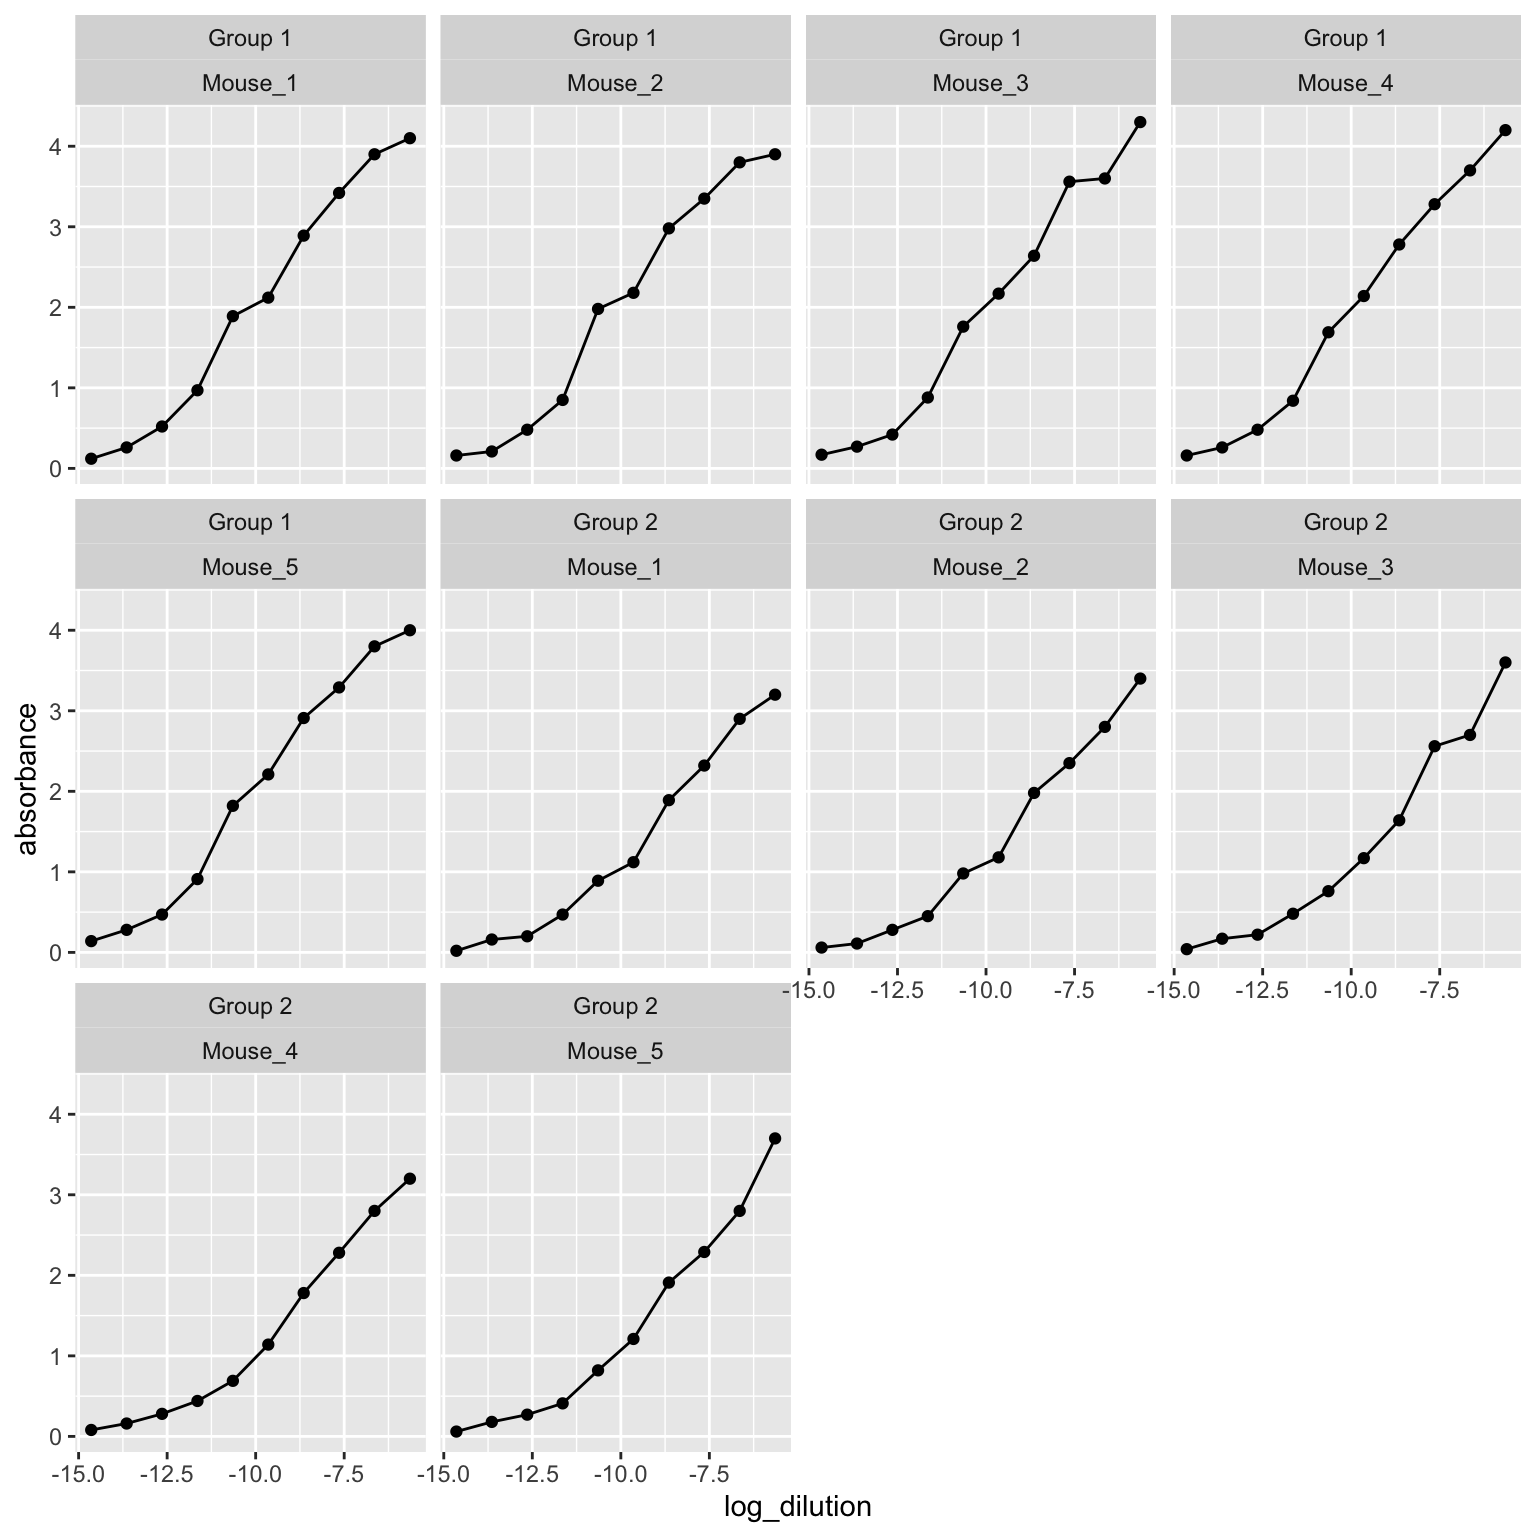
\includegraphics{csu-impactb_files/figure-latex/unnamed-chunk-39-1} \end{center}

Based on the curve, the values are:

a = 4,
d = 0
c = 2
b = 1

\hypertarget{creating-a-function-for-fitting-model}{%
\subsection{Creating a function for fitting model}\label{creating-a-function-for-fitting-model}}

\begin{Shaded}
\begin{Highlighting}[]
\NormalTok{fitted\_model\_elisa }\OtherTok{\textless{}{-}} \ControlFlowTok{function}\NormalTok{(df\_elisa, }
\NormalTok{                               start\_a, start\_d, }
\NormalTok{                               start\_c, start\_b) \{}
\NormalTok{  mod\_1 }\OtherTok{\textless{}{-}} \FunctionTok{nlsLM}\NormalTok{(absorbance }\SpecialCharTok{\textasciitilde{}} 
\NormalTok{                   ((a}\SpecialCharTok{{-}}\NormalTok{d)}\SpecialCharTok{/}\NormalTok{(}\DecValTok{1}\SpecialCharTok{+}\NormalTok{(log\_dilution}\SpecialCharTok{/}\NormalTok{c)}\SpecialCharTok{\^{}}\NormalTok{b)) }\SpecialCharTok{+}\NormalTok{ d,}
\AttributeTok{data =}\NormalTok{ df\_elisa,}
\AttributeTok{start =} \FunctionTok{list}\NormalTok{(}\AttributeTok{a =}\NormalTok{ start\_a, }\AttributeTok{d =}\NormalTok{ start\_d, }\AttributeTok{c =}\NormalTok{ start\_c, }\AttributeTok{b =}\NormalTok{ start\_b))}
  \FunctionTok{return}\NormalTok{(mod\_1)}
\NormalTok{\}}
\end{Highlighting}
\end{Shaded}

\hypertarget{fitting-the-model-into-the-dataset}{%
\subsubsection{Fitting the model into the dataset}\label{fitting-the-model-into-the-dataset}}

\begin{Shaded}
\begin{Highlighting}[]
\FunctionTok{fitted\_model\_elisa}\NormalTok{(elisa\_data\_nested}\SpecialCharTok{$}\NormalTok{data[[}\DecValTok{1}\NormalTok{]], }
                   \AttributeTok{start\_a =} \DecValTok{4}\NormalTok{, }
                   \AttributeTok{start\_d =} \DecValTok{0}\NormalTok{, }
                   \AttributeTok{start\_c =} \SpecialCharTok{{-}}\DecValTok{8}\NormalTok{, }
                   \AttributeTok{start\_b =} \DecValTok{1}\NormalTok{)}
\end{Highlighting}
\end{Shaded}

\begin{verbatim}
## Nonlinear regression model
##   model: absorbance ~ ((a - d)/(1 + (log_dilution/c)^b)) + d
##    data: df_elisa
##        a        d        c        b 
##   4.3070  -0.6009 -10.2577   5.2893 
##  residual sum-of-squares: 0.1199
## 
## Number of iterations to convergence: 7 
## Achieved convergence tolerance: 1.49e-08
\end{verbatim}

\hypertarget{apply-the-fitted-model-function-to-the-whole-dataframe}{%
\subsubsection{Apply the fitted model function to the whole dataframe}\label{apply-the-fitted-model-function-to-the-whole-dataframe}}

\begin{Shaded}
\begin{Highlighting}[]
\NormalTok{elisa\_fitted\_data }\OtherTok{\textless{}{-}}\NormalTok{ elisa\_data\_nested }\SpecialCharTok{\%\textgreater{}\%}
  \FunctionTok{mutate}\NormalTok{(}\AttributeTok{fitted\_data =} 
\NormalTok{           purrr}\SpecialCharTok{::}\FunctionTok{map}\NormalTok{(data, }\SpecialCharTok{\textasciitilde{}} 
                        \FunctionTok{fitted\_model\_elisa}\NormalTok{(.x,}\AttributeTok{start\_a =} \DecValTok{4}\NormalTok{, }
                                              \AttributeTok{start\_d =} \DecValTok{0}\NormalTok{, }
                                              \AttributeTok{start\_c =} \SpecialCharTok{{-}}\DecValTok{8}\NormalTok{, }
                                              \AttributeTok{start\_b =} \DecValTok{1}\NormalTok{)))}

\FunctionTok{head}\NormalTok{(elisa\_fitted\_data)}
\end{Highlighting}
\end{Shaded}

\begin{verbatim}
## # A tibble: 6 x 4
## # Groups:   Groups, mouse_id [6]
##   Groups  mouse_id data              fitted_data
##   <chr>   <chr>    <list>            <list>     
## 1 Group 1 Mouse_1  <tibble [10 x 5]> <nls>      
## 2 Group 1 Mouse_2  <tibble [10 x 5]> <nls>      
## 3 Group 1 Mouse_3  <tibble [10 x 5]> <nls>      
## 4 Group 1 Mouse_4  <tibble [10 x 5]> <nls>      
## 5 Group 1 Mouse_5  <tibble [10 x 5]> <nls>      
## 6 Group 2 Mouse_1  <tibble [10 x 5]> <nls>
\end{verbatim}

\hypertarget{take-out-the-summary-of-the-data}{%
\subsubsection{Take out the summary of the data}\label{take-out-the-summary-of-the-data}}

\begin{Shaded}
\begin{Highlighting}[]
\NormalTok{elisa\_fitted\_data\_summary }\OtherTok{\textless{}{-}}\NormalTok{ elisa\_fitted\_data }\SpecialCharTok{\%\textgreater{}\%}
  \FunctionTok{mutate}\NormalTok{(}\AttributeTok{elisa\_fitted\_data\_summary =} 
\NormalTok{           purrr}\SpecialCharTok{::}\FunctionTok{map}\NormalTok{(fitted\_data, broom}\SpecialCharTok{::}\NormalTok{glance))}

\NormalTok{unnested }\OtherTok{\textless{}{-}}\NormalTok{ elisa\_fitted\_data\_summary }\SpecialCharTok{\%\textgreater{}\%}
\FunctionTok{unnest}\NormalTok{(elisa\_fitted\_data\_summary) }\SpecialCharTok{\%\textgreater{}\%}
\FunctionTok{ungroup}\NormalTok{() }\SpecialCharTok{\%\textgreater{}\%}
\NormalTok{dplyr}\SpecialCharTok{::}\FunctionTok{select}\NormalTok{(Groups, mouse\_id, fitted\_data)}

\NormalTok{unnested}\SpecialCharTok{$}\NormalTok{fitted\_data[[}\DecValTok{1}\NormalTok{]]}
\end{Highlighting}
\end{Shaded}

\begin{verbatim}
## Nonlinear regression model
##   model: absorbance ~ ((a - d)/(1 + (log_dilution/c)^b)) + d
##    data: df_elisa
##        a        d        c        b 
##   4.3070  -0.6009 -10.2577   5.2893 
##  residual sum-of-squares: 0.1199
## 
## Number of iterations to convergence: 7 
## Achieved convergence tolerance: 1.49e-08
\end{verbatim}

\hypertarget{create-function-of-fitted-model-and-endpoint-titer-where-the-output-of-the-fitted-model-data-will-be-the-input-of-the-endpoint-titer}{%
\section{Create function of Fitted model and endpoint titer, where the output of the fitted model data will be the input of the endpoint titer}\label{create-function-of-fitted-model-and-endpoint-titer-where-the-output-of-the-fitted-model-data-will-be-the-input-of-the-endpoint-titer}}

\begin{Shaded}
\begin{Highlighting}[]
\CommentTok{\# Fitted model function}
\NormalTok{fitted\_model\_elisa }\OtherTok{\textless{}{-}} \ControlFlowTok{function}\NormalTok{(df\_elisa, }
\NormalTok{                               start\_a, }
\NormalTok{                               start\_d, }
\NormalTok{                               start\_c, }
\NormalTok{                               start\_b) \{}
\NormalTok{  mod\_1 }\OtherTok{\textless{}{-}} \FunctionTok{nlsLM}\NormalTok{(absorbance }\SpecialCharTok{\textasciitilde{}} 
\NormalTok{                   ((a}\SpecialCharTok{{-}}\NormalTok{d)}\SpecialCharTok{/}\NormalTok{(}\DecValTok{1}\SpecialCharTok{+}\NormalTok{(log\_dilution}\SpecialCharTok{/}\NormalTok{c)}\SpecialCharTok{\^{}}\NormalTok{b)) }\SpecialCharTok{+}\NormalTok{ d,}
\AttributeTok{data =}\NormalTok{ df\_elisa,}
\AttributeTok{start =} \FunctionTok{list}\NormalTok{(}\AttributeTok{a =}\NormalTok{ start\_a, }\AttributeTok{d =}\NormalTok{ start\_d, }\AttributeTok{c =}\NormalTok{ start\_c, }\AttributeTok{b =}\NormalTok{ start\_b))}
  \FunctionTok{return}\NormalTok{(mod\_1)}
\NormalTok{\}}

\CommentTok{\# Endpoint titer function}

\NormalTok{endpoint\_titer\_elisa }\OtherTok{\textless{}{-}} \ControlFlowTok{function}\NormalTok{(fitted\_data, back\_value) \{}
\NormalTok{  tidy\_fitted }\OtherTok{\textless{}{-}}\NormalTok{ broom}\SpecialCharTok{::}\FunctionTok{tidy}\NormalTok{(fitted\_data)}
\NormalTok{  est\_a }\OtherTok{\textless{}{-}}\NormalTok{ tidy\_fitted}\SpecialCharTok{$}\NormalTok{estimate[tidy\_fitted}\SpecialCharTok{$}\NormalTok{term }\SpecialCharTok{==} \StringTok{"a"}\NormalTok{]}
\NormalTok{  est\_b }\OtherTok{\textless{}{-}}\NormalTok{ tidy\_fitted}\SpecialCharTok{$}\NormalTok{estimate[tidy\_fitted}\SpecialCharTok{$}\NormalTok{term }\SpecialCharTok{==} \StringTok{"b"}\NormalTok{]}
\NormalTok{  est\_c }\OtherTok{\textless{}{-}}\NormalTok{ tidy\_fitted}\SpecialCharTok{$}\NormalTok{estimate[tidy\_fitted}\SpecialCharTok{$}\NormalTok{term }\SpecialCharTok{==} \StringTok{"c"}\NormalTok{]}
\NormalTok{  est\_d }\OtherTok{\textless{}{-}}\NormalTok{ tidy\_fitted}\SpecialCharTok{$}\NormalTok{estimate[tidy\_fitted}\SpecialCharTok{$}\NormalTok{term }\SpecialCharTok{==} \StringTok{"d"}\NormalTok{]}
\NormalTok{  endpoint\_titer }\OtherTok{\textless{}{-}}\NormalTok{ est\_c }\SpecialCharTok{*}\NormalTok{ (((est\_a }\SpecialCharTok{{-}}\NormalTok{ est\_d) }\SpecialCharTok{/}\NormalTok{ (back\_value }\SpecialCharTok{{-}}\NormalTok{ est\_d)) }\SpecialCharTok{{-}} \DecValTok{1}\NormalTok{) }\SpecialCharTok{\^{}}\NormalTok{ (}\DecValTok{1} \SpecialCharTok{/}\NormalTok{ est\_b)}
  \FunctionTok{return}\NormalTok{(endpoint\_titer)}
\NormalTok{\}}
\end{Highlighting}
\end{Shaded}

\hypertarget{apply-the-fitted-model-fuction-into-the-nested-data-and-use-the-output-of-the-fitted-data-as-the-input-for-endpoint-titer-value-evaluation}{%
\subsubsection{Apply the fitted model fuction into the nested data and use the output of the fitted data as the input for endpoint titer value evaluation}\label{apply-the-fitted-model-fuction-into-the-nested-data-and-use-the-output-of-the-fitted-data-as-the-input-for-endpoint-titer-value-evaluation}}

\hypertarget{run-fitted-model-on-the-data}{%
\paragraph{Run fitted model on the data}\label{run-fitted-model-on-the-data}}

\begin{Shaded}
\begin{Highlighting}[]
\NormalTok{elisa\_data\_with\_fit\_model }\OtherTok{\textless{}{-}}\NormalTok{ elisa\_data\_nested }\SpecialCharTok{\%\textgreater{}\%}
  \FunctionTok{mutate}\NormalTok{(}\AttributeTok{fitted\_data =}\NormalTok{ purrr}\SpecialCharTok{::}\FunctionTok{map}\NormalTok{(data, }
                                  \SpecialCharTok{\textasciitilde{}} \FunctionTok{fitted\_model\_elisa}\NormalTok{(.x, }\AttributeTok{start\_a =} \DecValTok{4}\NormalTok{, }
                                                          \AttributeTok{start\_d =} \DecValTok{0}\NormalTok{, }
                                                          \AttributeTok{start\_c =} \SpecialCharTok{{-}}\DecValTok{8}\NormalTok{, }
                                                          \AttributeTok{start\_b =} \DecValTok{1}\NormalTok{)))}

\FunctionTok{head}\NormalTok{(elisa\_data\_with\_fit\_model)}
\end{Highlighting}
\end{Shaded}

\begin{verbatim}
## # A tibble: 6 x 4
## # Groups:   Groups, mouse_id [6]
##   Groups  mouse_id data              fitted_data
##   <chr>   <chr>    <list>            <list>     
## 1 Group 1 Mouse_1  <tibble [10 x 5]> <nls>      
## 2 Group 1 Mouse_2  <tibble [10 x 5]> <nls>      
## 3 Group 1 Mouse_3  <tibble [10 x 5]> <nls>      
## 4 Group 1 Mouse_4  <tibble [10 x 5]> <nls>      
## 5 Group 1 Mouse_5  <tibble [10 x 5]> <nls>      
## 6 Group 2 Mouse_1  <tibble [10 x 5]> <nls>
\end{verbatim}

\hypertarget{taking-output-of-the-fitted-model-function-and-into-endpoint-titer-function}{%
\paragraph{Taking output of the fitted model function and into endpoint titer function}\label{taking-output-of-the-fitted-model-function-and-into-endpoint-titer-function}}

\begin{Shaded}
\begin{Highlighting}[]
\NormalTok{elisa\_data\_with\_endpoint\_titer }\OtherTok{\textless{}{-}}\NormalTok{ elisa\_data\_with\_fit\_model }\SpecialCharTok{\%\textgreater{}\%}
  \FunctionTok{mutate}\NormalTok{(}\AttributeTok{endpoint\_data =} 
\NormalTok{           purrr}\SpecialCharTok{::}\FunctionTok{map}\NormalTok{(fitted\_data, }
                      \SpecialCharTok{\textasciitilde{}} \FunctionTok{endpoint\_titer\_elisa}\NormalTok{(.x, }\AttributeTok{back\_value =} \FloatTok{0.2}\NormalTok{)))}
\end{Highlighting}
\end{Shaded}

\hypertarget{plot-the-endpoint-titer-data-for-the-two-groups}{%
\subsubsection{Plot the endpoint titer data for the two groups}\label{plot-the-endpoint-titer-data-for-the-two-groups}}

\begin{Shaded}
\begin{Highlighting}[]
\NormalTok{elisa\_data\_with\_endpoint\_titer}\SpecialCharTok{$}\NormalTok{endpoint\_data}\OtherTok{=}
  \FunctionTok{as.numeric}\NormalTok{(elisa\_data\_with\_endpoint\_titer}\SpecialCharTok{$}\NormalTok{endpoint\_data)}

\NormalTok{elisa\_data\_with\_endpoint\_titer }\SpecialCharTok{\%\textgreater{}\%}
  \FunctionTok{ggplot}\NormalTok{(}\FunctionTok{aes}\NormalTok{(}\AttributeTok{x =}\NormalTok{ Groups, }\AttributeTok{y =}\NormalTok{ endpoint\_data, }\AttributeTok{color =}\NormalTok{ Groups)) }\SpecialCharTok{+}
 \FunctionTok{geom\_beeswarm}\NormalTok{(}\AttributeTok{cex =} \DecValTok{3}\NormalTok{) }
\end{Highlighting}
\end{Shaded}

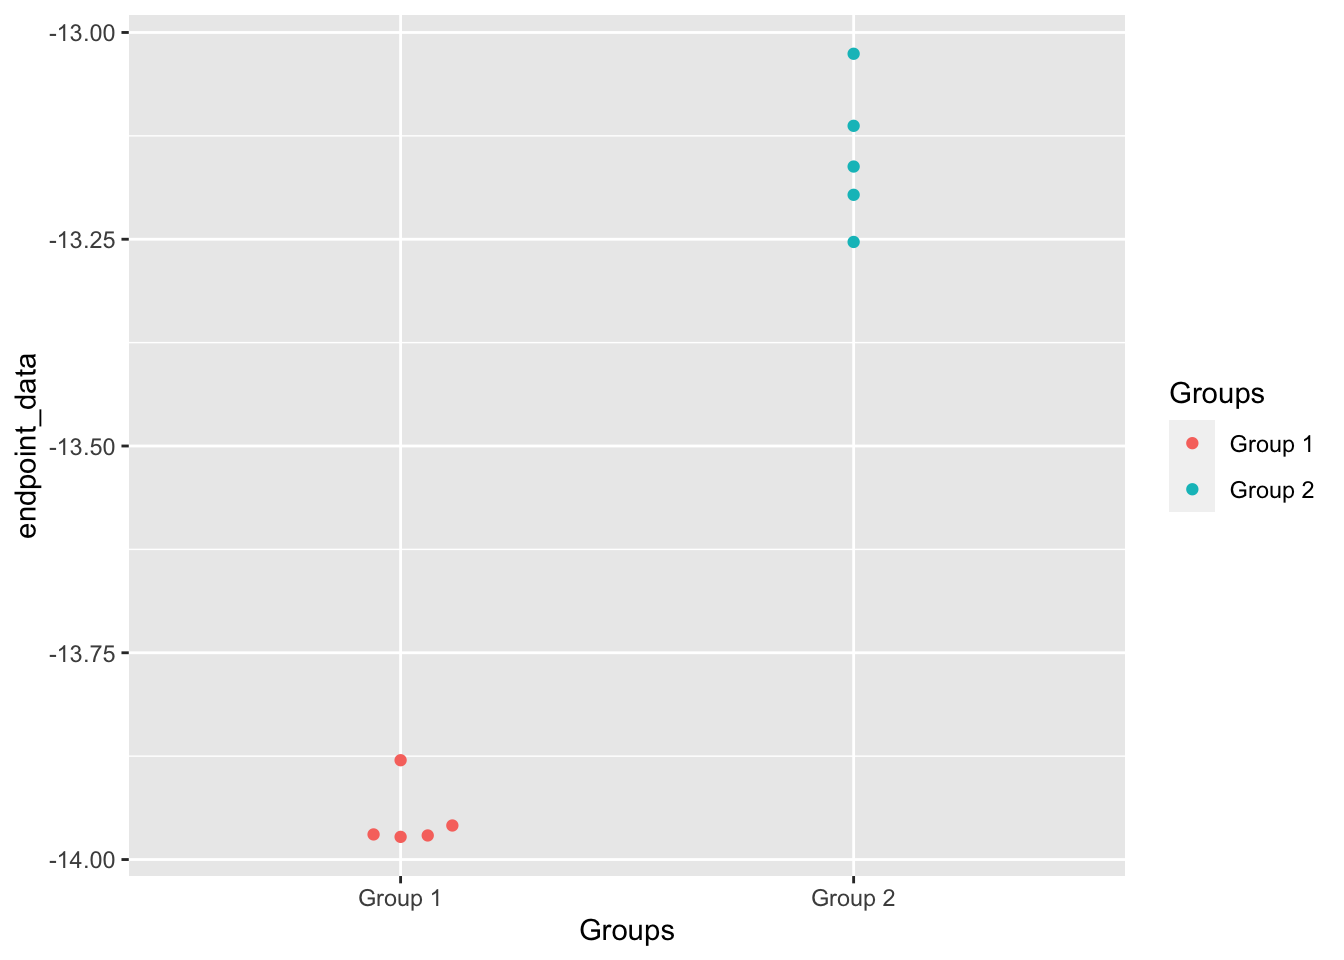
\includegraphics{csu-impactb_files/figure-latex/unnamed-chunk-47-1.pdf}

\hypertarget{perform-statistical-analysis-on-the-data}{%
\subsubsection{Perform statistical analysis on the data}\label{perform-statistical-analysis-on-the-data}}

\begin{Shaded}
\begin{Highlighting}[]
\NormalTok{elisa\_data\_stats }\OtherTok{\textless{}{-}} \FunctionTok{t.test}\NormalTok{(endpoint\_data }\SpecialCharTok{\textasciitilde{}}\NormalTok{ Groups, }
                           \AttributeTok{data =}\NormalTok{ elisa\_data\_with\_endpoint\_titer)}

\NormalTok{elisa\_data\_stats }\SpecialCharTok{\%\textgreater{}\%}
  \FunctionTok{tidy}\NormalTok{()}
\end{Highlighting}
\end{Shaded}

\begin{verbatim}
## # A tibble: 1 x 10
##   estimate estimate1 estimate2 statistic    p.value parameter conf.low conf.high
##      <dbl>     <dbl>     <dbl>     <dbl>      <dbl>     <dbl>    <dbl>     <dbl>
## 1   -0.800     -14.0     -13.2     -18.8 0.00000268      5.63   -0.906    -0.695
## # ... with 2 more variables: method <chr>, alternative <chr>
\end{verbatim}

\hypertarget{statistical-data-analysis-for-more-than-two-groups}{%
\subsubsection{Statistical data analysis for more than two groups}\label{statistical-data-analysis-for-more-than-two-groups}}

\hypertarget{elisa-data-processing}{%
\section{ELISA data processing}\label{elisa-data-processing}}

We read ELISA plate in a 96 well plate using a plate reader. The plate reader generates the data in form of number in an excel sheet. We have created this pipeline/worksheet to bring out the information from the excl sheet to a tidy format in which the above created fitted model and endpoint titer functions can be applied.

\hypertarget{read-in-the-first-dataset}{%
\subsubsection{Read in the first dataset}\label{read-in-the-first-dataset}}

Below is the example ELISA data that has came straight out of the plate reader. This data is arranged in a 96-well plate format and contains Optical Density (OD) values.

\begin{Shaded}
\begin{Highlighting}[]
\NormalTok{elisa\_raw\_data }\OtherTok{\textless{}{-}} \FunctionTok{read\_excel}\NormalTok{(}\StringTok{"DATA/elisa\_s1\_07{-}25{-}20.xlsx"}\NormalTok{, }
                             \AttributeTok{sheet =} \StringTok{"S1"}\NormalTok{, }\AttributeTok{col\_names =} \ConstantTok{FALSE}\NormalTok{,  }
                             \AttributeTok{range =} \StringTok{"B2:M9"}\NormalTok{)}
\end{Highlighting}
\end{Shaded}

\begin{verbatim}
## New names:
## * `` -> ...1
## * `` -> ...2
## * `` -> ...3
## * `` -> ...4
## * `` -> ...5
## * ...
\end{verbatim}

\begin{Shaded}
\begin{Highlighting}[]
\FunctionTok{head}\NormalTok{(elisa\_raw\_data)}
\end{Highlighting}
\end{Shaded}

\begin{verbatim}
## # A tibble: 6 x 12
##   ...1          ...2  ...3 ...4   ...5  ...6 ...7   ...8  ...9 ...10 ...11 ...12
##   <chr>        <dbl> <dbl> <chr> <dbl> <dbl> <chr> <dbl> <dbl> <chr> <dbl> <dbl>
## 1 5.199999999~ 0.05  0.069 6.3E~ 0.061 0.122 0.16~ 0.145 0.135 6.80~ 0.053 0.05 
## 2 7.900000000~ 0.098 0.069 6.80~ 0.115 0.202 5.89~ 0.134 0.069 0.106 0.05  0.075
## 3 8.899999999~ 0.133 0.119 OVRF~ 3.87  2.32  OVRF~ 3.85  2.12  OVRF~ 3.21  1.02 
## 4 OVRFLW       3.46  1.16  OVRF~ 3.80  2.36  OVRF~ 3.70  1.49  OVRF~ 3.68  1.63 
## 5 3.815999999~ 1.82  0.446 3.89~ 3.42  1.13  OVRF~ 2.33  0.608 OVRF~ 3.41  1.10 
## 6 OVRFLW       3.69  1.43  OVRF~ 3.66  1.27  3.839 1.74  0.444 2.49~ 0.637 0.704
\end{verbatim}

\hypertarget{tidy-dataset-1}{%
\subsubsection{Tidy dataset 1}\label{tidy-dataset-1}}

It is important to clean the data and arrange it in a format on which we can apply formulas and functions.

\begin{Shaded}
\begin{Highlighting}[]
\CommentTok{\# Convert all columns to numeric}

\NormalTok{elisa\_raw\_data\_numeric }\OtherTok{\textless{}{-}}\NormalTok{ elisa\_raw\_data }\SpecialCharTok{\%\textgreater{}\%} 
  \FunctionTok{mutate\_if}\NormalTok{(is.character, as.numeric)}
\end{Highlighting}
\end{Shaded}

\begin{verbatim}
## Warning in mask$eval_all_mutate(quo): NAs introduced by coercion

## Warning in mask$eval_all_mutate(quo): NAs introduced by coercion

## Warning in mask$eval_all_mutate(quo): NAs introduced by coercion

## Warning in mask$eval_all_mutate(quo): NAs introduced by coercion
\end{verbatim}

\begin{Shaded}
\begin{Highlighting}[]
\CommentTok{\# pivot longer the data}

\NormalTok{elisa\_raw\_data\_tidy }\OtherTok{\textless{}{-}} \FunctionTok{pivot\_longer}\NormalTok{(}\AttributeTok{data =}\NormalTok{ elisa\_raw\_data\_numeric, }\AttributeTok{cols =} \StringTok{"...1"}\SpecialCharTok{:}\StringTok{"...12"}\NormalTok{, }\AttributeTok{names\_to =} \StringTok{"well\_id"}\NormalTok{, }\AttributeTok{values\_to =} \StringTok{"od\_450nm"}\NormalTok{)}

\CommentTok{\# remove "..." from the first column}

\NormalTok{elisa\_raw\_data\_tidy}\SpecialCharTok{$}\NormalTok{well\_id }\OtherTok{\textless{}{-}} \FunctionTok{str\_replace}\NormalTok{(elisa\_raw\_data\_tidy}\SpecialCharTok{$}\NormalTok{well\_id, }\StringTok{"..."}\NormalTok{, }\StringTok{""}\NormalTok{)}

\CommentTok{\# Add new column to the data\_frame}

\NormalTok{elisa\_raw\_data\_tidy\_new }\OtherTok{\textless{}{-}}\NormalTok{ elisa\_raw\_data\_tidy }\SpecialCharTok{\%\textgreater{}\%}
  \FunctionTok{mutate}\NormalTok{(}\AttributeTok{name =} \FunctionTok{rep}\NormalTok{(LETTERS[}\DecValTok{1}\SpecialCharTok{:}\DecValTok{8}\NormalTok{], }\AttributeTok{each =} \DecValTok{12}\NormalTok{))}

\NormalTok{elisa\_raw\_data\_tidy\_new }\OtherTok{\textless{}{-}}\NormalTok{ elisa\_raw\_data\_tidy\_new }\SpecialCharTok{\%\textgreater{}\%}
  \FunctionTok{mutate}\NormalTok{(}\AttributeTok{well\_id =} \FunctionTok{paste0}\NormalTok{(name, well\_id)) }\SpecialCharTok{\%\textgreater{}\%}
  \FunctionTok{select}\NormalTok{(}\SpecialCharTok{{-}}\NormalTok{name)}

\FunctionTok{head}\NormalTok{(elisa\_raw\_data\_tidy\_new)}
\end{Highlighting}
\end{Shaded}

\begin{verbatim}
## # A tibble: 6 x 2
##   well_id od_450nm
##   <chr>      <dbl>
## 1 A1         0.052
## 2 A2         0.05 
## 3 A3         0.069
## 4 A4         0.063
## 5 A5         0.061
## 6 A6         0.122
\end{verbatim}

\hypertarget{read-in-the-second-data-set}{%
\subsubsection{Read in the second data set}\label{read-in-the-second-data-set}}

The second dataset contains the information such as groups, mouse id, and dilutions for the respective wells of the 96 well plate for the dataset-1.

\begin{Shaded}
\begin{Highlighting}[]
\NormalTok{elisa\_label\_data }\OtherTok{\textless{}{-}} \FunctionTok{read\_excel}\NormalTok{(}\StringTok{"DATA/elisa\_s1\_07{-}25{-}20.xlsx"}\NormalTok{, }
                               \AttributeTok{sheet =} \StringTok{"S1"}\NormalTok{, }\AttributeTok{col\_names =} \ConstantTok{FALSE}\NormalTok{,  }
                               \AttributeTok{range =} \StringTok{"Q2:AB9"}\NormalTok{)}
\end{Highlighting}
\end{Shaded}

\begin{verbatim}
## New names:
## * `` -> ...1
## * `` -> ...2
## * `` -> ...3
## * `` -> ...4
## * `` -> ...5
## * ...
\end{verbatim}

\begin{Shaded}
\begin{Highlighting}[]
\FunctionTok{head}\NormalTok{(elisa\_label\_data)}
\end{Highlighting}
\end{Shaded}

\begin{verbatim}
## # A tibble: 6 x 12
##   ...1        ...2   ...3  ...4  ...5  ...6  ...7  ...8  ...9  ...10 ...11 ...12
##   <chr>       <chr>  <chr> <chr> <chr> <chr> <chr> <chr> <chr> <chr> <chr> <chr>
## 1 blank       secon~ naïv~ 1A-1~ 1A-1~ 1A-1~ 1A-2~ 1A-2~ 1A-2~ 1A-3~ 1A-3~ 1A-3~
## 2 1A-4 (1/250 1A-4 ~ 1A-4~ 1B-1~ 1B-1~ 1B-1~ 1B-2~ 1B-2~ 1B-2~ 1B-3~ 1B-3~ 1B-3~
## 3 1B-4 (1/250 1B-4 ~ 1B-4~ 2A-1~ 2A-1~ 2A-1~ 2A-2~ 2A-2~ 2A-2~ 2A-3~ 2A-3~ 2A-3~
## 4 2B-1 (1/250 2B-1 ~ 2B-1~ 2B-2~ 2B-2~ 2B-2~ 2B-3~ 2B-3~ 2B-3~ 2B-4~ 2B-4~ 2B-4~
## 5 3A-1 (1/250 3A-1 ~ 3A-1~ 3A-2~ 3A-2~ 3A-2~ 3A-3~ 3A-3~ 3A-3~ 3A-4~ 3A-4~ 3A-4~
## 6 3B-1 (1/250 3B-1 ~ 3B-1~ 3B-2~ 3B-2~ 3B-2~ 3B-3~ 3B-3~ 3B-3~ 3B-4~ 3B-4~ 3B-4~
\end{verbatim}

\hypertarget{tidy-dataset-2}{%
\subsubsection{Tidy dataset-2}\label{tidy-dataset-2}}

\begin{Shaded}
\begin{Highlighting}[]
\CommentTok{\# pivot longer the data}

\NormalTok{elisa\_label\_data\_tidy }\OtherTok{\textless{}{-}} \FunctionTok{pivot\_longer}\NormalTok{(}\AttributeTok{data =}\NormalTok{ elisa\_label\_data, }
                                      \AttributeTok{cols =} \StringTok{"...1"}\SpecialCharTok{:}\StringTok{"...12"}\NormalTok{, }
                                      \AttributeTok{names\_to =} \StringTok{"well\_id"}\NormalTok{, }
                                      \AttributeTok{values\_to =} \StringTok{"information"}\NormalTok{)}

\CommentTok{\# remove "..." from the first column}

\NormalTok{elisa\_label\_data\_tidy}\SpecialCharTok{$}\NormalTok{well\_id }\OtherTok{\textless{}{-}} \FunctionTok{str\_replace}\NormalTok{(elisa\_label\_data\_tidy}\SpecialCharTok{$}\NormalTok{well\_id, }\StringTok{"..."}\NormalTok{, }\StringTok{""}\NormalTok{)}

\CommentTok{\# Add new column to the data\_frame}

\NormalTok{elisa\_label\_data\_tidy\_new }\OtherTok{\textless{}{-}}\NormalTok{ elisa\_label\_data\_tidy }\SpecialCharTok{\%\textgreater{}\%}
  \FunctionTok{mutate}\NormalTok{(}\AttributeTok{name =} \FunctionTok{rep}\NormalTok{(LETTERS[}\DecValTok{1}\SpecialCharTok{:}\DecValTok{8}\NormalTok{], }\AttributeTok{each =} \DecValTok{12}\NormalTok{))}

\NormalTok{elisa\_label\_data\_tidy\_new }\OtherTok{\textless{}{-}}\NormalTok{ elisa\_label\_data\_tidy\_new }\SpecialCharTok{\%\textgreater{}\%}
  \FunctionTok{mutate}\NormalTok{(}\AttributeTok{well\_id =} \FunctionTok{paste0}\NormalTok{(name, well\_id)) }\SpecialCharTok{\%\textgreater{}\%}
  \FunctionTok{select}\NormalTok{(}\SpecialCharTok{{-}}\NormalTok{name)}

\FunctionTok{head}\NormalTok{(elisa\_label\_data\_tidy\_new)}
\end{Highlighting}
\end{Shaded}

\begin{verbatim}
## # A tibble: 6 x 2
##   well_id information  
##   <chr>   <chr>        
## 1 A1      blank        
## 2 A2      secondary    
## 3 A3      naïve (1/250)
## 4 A4      1A-1 (1/250  
## 5 A5      1A-1 (1/1250 
## 6 A6      1A-1 (1/6250
\end{verbatim}

\hypertarget{merge-dataset-1-with-od-information-with-dataset-2-with-respective-data-information}{%
\subsubsection{Merge dataset-1 (with OD information) with dataset-2 (with respective data information)}\label{merge-dataset-1-with-od-information-with-dataset-2-with-respective-data-information}}

To create a complete full dataset with Groups, mouse-id, dilutions, and OD, we merged the dataset-1 and dataset-2 together. We also cleaned the data set so that mouse-ID and dilution columns are separate and have their own columns.

\begin{Shaded}
\begin{Highlighting}[]
\CommentTok{\#Merge the two datasets}

\NormalTok{elisa\_data }\OtherTok{=}\NormalTok{ elisa\_raw\_data\_tidy\_new }\SpecialCharTok{\%\textgreater{}\%} \FunctionTok{inner\_join}\NormalTok{(elisa\_label\_data\_tidy\_new,}
                                                    \AttributeTok{by=}\StringTok{"well\_id"}\NormalTok{)}

\FunctionTok{head}\NormalTok{(elisa\_data)}
\end{Highlighting}
\end{Shaded}

\begin{verbatim}
## # A tibble: 6 x 3
##   well_id od_450nm information  
##   <chr>      <dbl> <chr>        
## 1 A1         0.052 blank        
## 2 A2         0.05  secondary    
## 3 A3         0.069 naïve (1/250)
## 4 A4         0.063 1A-1 (1/250  
## 5 A5         0.061 1A-1 (1/1250 
## 6 A6         0.122 1A-1 (1/6250
\end{verbatim}

\begin{Shaded}
\begin{Highlighting}[]
\DocumentationTok{\#\#\# Separate the information table into sample ID and dilution columns}

\NormalTok{tidy\_elisa\_data }\OtherTok{\textless{}{-}} \FunctionTok{separate}\NormalTok{(elisa\_data, }\AttributeTok{col =} \StringTok{"information"}\NormalTok{, }
                            \AttributeTok{into =} \FunctionTok{c}\NormalTok{(}\StringTok{"sample\_id"}\NormalTok{, }\StringTok{"dilution"}\NormalTok{),}
                            \AttributeTok{sep =} \StringTok{"}\SpecialCharTok{\textbackslash{}\textbackslash{}}\StringTok{("}\NormalTok{)}
\end{Highlighting}
\end{Shaded}

\begin{verbatim}
## Warning: Expected 2 pieces. Missing pieces filled with `NA` in 2 rows [1, 2].
\end{verbatim}

\begin{Shaded}
\begin{Highlighting}[]
\FunctionTok{head}\NormalTok{(tidy\_elisa\_data)}
\end{Highlighting}
\end{Shaded}

\begin{verbatim}
## # A tibble: 6 x 4
##   well_id od_450nm sample_id   dilution
##   <chr>      <dbl> <chr>       <chr>   
## 1 A1         0.052 "blank"     <NA>    
## 2 A2         0.05  "secondary" <NA>    
## 3 A3         0.069 "naïve "    1/250)  
## 4 A4         0.063 "1A-1 "     1/250   
## 5 A5         0.061 "1A-1 "     1/1250  
## 6 A6         0.122 "1A-1 "     1/6250
\end{verbatim}

\begin{Shaded}
\begin{Highlighting}[]
\NormalTok{tidy\_elisa\_data }\OtherTok{\textless{}{-}}\NormalTok{ tidy\_elisa\_data }\SpecialCharTok{\%\textgreater{}\%}
  \FunctionTok{mutate}\NormalTok{(}\AttributeTok{dilution =} \FunctionTok{str\_extract}\NormalTok{(dilution, }\StringTok{"(/)[0{-}9]+"}\NormalTok{),}
         \AttributeTok{dilution =} \FunctionTok{str\_replace}\NormalTok{(dilution, }\StringTok{"/"}\NormalTok{, }\StringTok{""}\NormalTok{),}
         \AttributeTok{dilution =} \FunctionTok{as.numeric}\NormalTok{(dilution))}

\NormalTok{tidy\_elisa\_data }\OtherTok{\textless{}{-}}\NormalTok{ tidy\_elisa\_data }\SpecialCharTok{\%\textgreater{}\%}
  \FunctionTok{select}\NormalTok{(well\_id, sample\_id, dilution, od\_450nm)}

\FunctionTok{head}\NormalTok{(tidy\_elisa\_data)}
\end{Highlighting}
\end{Shaded}

\begin{verbatim}
## # A tibble: 6 x 4
##   well_id sample_id   dilution od_450nm
##   <chr>   <chr>          <dbl>    <dbl>
## 1 A1      "blank"           NA    0.052
## 2 A2      "secondary"       NA    0.05 
## 3 A3      "naïve "         250    0.069
## 4 A4      "1A-1 "          250    0.063
## 5 A5      "1A-1 "         1250    0.061
## 6 A6      "1A-1 "         6250    0.122
\end{verbatim}

\hypertarget{flow-cytometry}{%
\chapter{Flow cytometry}\label{flow-cytometry}}

Flow cytometry data can be quantified in many different ways and with different techniques. For the purpose of these data analyses, manual gating has been achieved in FlowJo and cell frequencies and populations exported as a \texttt{.csv} file. This \texttt{.csv} file is the primary input for this R pipeline which aims to output box plots for each gated cell population.

This example data set is from an innate response study whcih investigated the immune response in the lungs during the first 28 days of infection.

\hypertarget{loading-packages}{%
\section{Loading packages}\label{loading-packages}}

\begin{Shaded}
\begin{Highlighting}[]
\FunctionTok{library}\NormalTok{(readxl)}
\FunctionTok{library}\NormalTok{(ggplot2)}
\FunctionTok{library}\NormalTok{(RColorBrewer)}
\FunctionTok{library}\NormalTok{(dplyr)}
\FunctionTok{library}\NormalTok{(tidyverse)}
\FunctionTok{library}\NormalTok{(scales)}
\end{Highlighting}
\end{Shaded}

\begin{verbatim}
## 
## Attaching package: 'scales'
\end{verbatim}

\begin{verbatim}
## The following object is masked from 'package:purrr':
## 
##     discard
\end{verbatim}

\begin{verbatim}
## The following object is masked from 'package:readr':
## 
##     col_factor
\end{verbatim}

\begin{Shaded}
\begin{Highlighting}[]
\FunctionTok{library}\NormalTok{(stringr)}
\FunctionTok{library}\NormalTok{(tidyr)}
\FunctionTok{library}\NormalTok{(knitr)}
\FunctionTok{library}\NormalTok{(forcats)}
\FunctionTok{library}\NormalTok{(broom)}
\FunctionTok{library}\NormalTok{(ggfortify)}
\FunctionTok{library}\NormalTok{(stats)}
\FunctionTok{library}\NormalTok{(ggpubr)}
\FunctionTok{library}\NormalTok{(grDevices)}
\FunctionTok{library}\NormalTok{(rstatix)}
\end{Highlighting}
\end{Shaded}

\begin{verbatim}
## 
## Attaching package: 'rstatix'
\end{verbatim}

\begin{verbatim}
## The following object is masked from 'package:stats':
## 
##     filter
\end{verbatim}

\begin{Shaded}
\begin{Highlighting}[]
\FunctionTok{library}\NormalTok{(writexl)}
\end{Highlighting}
\end{Shaded}

\hypertarget{panel-information}{%
\section{panel information}\label{panel-information}}

\begin{Shaded}
\begin{Highlighting}[]
\CommentTok{\# antibody\_panel \textless{}{-} read\_excel}
\end{Highlighting}
\end{Shaded}

\hypertarget{loading-data}{%
\section{Loading data}\label{loading-data}}

\begin{Shaded}
\begin{Highlighting}[]
\NormalTok{Df }\OtherTok{\textless{}{-}} \FunctionTok{read\_excel}\NormalTok{(}\StringTok{"DATA/innate\_normalizedto45.xlsx"}\NormalTok{, }\AttributeTok{sheet =} \StringTok{"CD3CD11b No Day 14"}\NormalTok{)}

\NormalTok{marker\_legend }\OtherTok{\textless{}{-}} \FunctionTok{read\_excel}\NormalTok{(}\StringTok{"DATA/marker legend.xlsx"}\NormalTok{)}

\CommentTok{\# Remove Freq of Parent columns}
\NormalTok{Df1 }\OtherTok{\textless{}{-}}\NormalTok{ Df }\SpecialCharTok{\%\textgreater{}\%} 
  \FunctionTok{select}\NormalTok{(}\SpecialCharTok{{-}}\FunctionTok{matches}\NormalTok{(}\StringTok{"Parent"}\NormalTok{))}
\CommentTok{\# Remove "Leukocytes/LIVE/Single Cells/" from col names}
\FunctionTok{names}\NormalTok{(Df1) }\OtherTok{\textless{}{-}} \FunctionTok{str\_remove}\NormalTok{(}\FunctionTok{names}\NormalTok{(Df1), }\StringTok{"Leukocytes/LIVE/Single Cells/"}\NormalTok{)}

\NormalTok{Df1 }\OtherTok{\textless{}{-}}\NormalTok{ Df1 }\SpecialCharTok{\%\textgreater{}\%}
  \FunctionTok{rename\_all}\NormalTok{(}\FunctionTok{funs}\NormalTok{(}\FunctionTok{str\_replace}\NormalTok{(., }\StringTok{"}\SpecialCharTok{\textbackslash{}\textbackslash{}}\StringTok{|.+"}\NormalTok{, }\StringTok{""}\NormalTok{)))}\CommentTok{\# Remove "|Freq of..." from col names}
\end{Highlighting}
\end{Shaded}

\begin{verbatim}
## Warning: `funs()` was deprecated in dplyr 0.8.0.
## Please use a list of either functions or lambdas: 
## 
##   # Simple named list: 
##   list(mean = mean, median = median)
## 
##   # Auto named with `tibble::lst()`: 
##   tibble::lst(mean, median)
## 
##   # Using lambdas
##   list(~ mean(., trim = .2), ~ median(., na.rm = TRUE))
## This warning is displayed once every 8 hours.
## Call `lifecycle::last_lifecycle_warnings()` to see where this warning was generated.
\end{verbatim}

\begin{Shaded}
\begin{Highlighting}[]
\NormalTok{Df1 }\OtherTok{\textless{}{-}}\NormalTok{ Df1 }\SpecialCharTok{\%\textgreater{}\%}
  \FunctionTok{rename\_all}\NormalTok{(}\FunctionTok{funs}\NormalTok{(}\FunctionTok{str\_replace\_all}\NormalTok{(., }\StringTok{"}\SpecialCharTok{\textbackslash{}\textbackslash{}}\StringTok{/Q[:digit:]+}\SpecialCharTok{\textbackslash{}\textbackslash{}}\StringTok{:"}\NormalTok{, }\StringTok{""}\NormalTok{))) }\SpecialCharTok{\%\textgreater{}\%}
  \FunctionTok{rename\_all}\NormalTok{(}\FunctionTok{funs}\NormalTok{(}\FunctionTok{str\_replace}\NormalTok{(., }\StringTok{"}\SpecialCharTok{\textbackslash{}\textbackslash{}}\StringTok{/"}\NormalTok{, }\StringTok{" "}\NormalTok{))) }\SpecialCharTok{\%\textgreater{}\%}
  \FunctionTok{rename\_all}\NormalTok{(}\FunctionTok{funs}\NormalTok{(}\FunctionTok{str\_replace}\NormalTok{(., }\StringTok{"}\SpecialCharTok{\textbackslash{}\textbackslash{}}\StringTok{,"}\NormalTok{, }\StringTok{" "}\NormalTok{))) }\SpecialCharTok{\%\textgreater{}\%}
  \FunctionTok{rename\_all}\NormalTok{(}\FunctionTok{funs}\NormalTok{(}\FunctionTok{str\_replace}\NormalTok{(., }\StringTok{"}\SpecialCharTok{\textbackslash{}\textbackslash{}}\StringTok{ }\SpecialCharTok{\textbackslash{}\textbackslash{}}\StringTok{,"}\NormalTok{, }\StringTok{" "}\NormalTok{)))}

\CommentTok{\# str\_extract\_all(names(Df1), "[:alpha:]+[:digit:]+[\textbackslash{}\textbackslash{}+\textbackslash{}\textbackslash{}{-}]")}
\CommentTok{\# }
\CommentTok{\# }
\CommentTok{\# }
\CommentTok{\# }
\CommentTok{\# }
\CommentTok{\# }
\CommentTok{\# marker\_select \textless{}{-} function(col\_title) \{}
\CommentTok{\#   marker\_df \textless{}{-} str\_detect(names(DATA1), "[\textbackslash{}\textbackslash{}+\textbackslash{}\textbackslash{}{-}]") }
\CommentTok{\#   return(marker\_df)}
\CommentTok{\# \}}
\end{Highlighting}
\end{Shaded}

\hypertarget{making-the-data-tidy-for-plotting}{%
\section{Making the data tidy for plotting}\label{making-the-data-tidy-for-plotting}}

\begin{Shaded}
\begin{Highlighting}[]
\NormalTok{tidy\_Df1 }\OtherTok{\textless{}{-}} \FunctionTok{pivot\_longer}\NormalTok{(}\AttributeTok{data =}\NormalTok{ Df1, }\AttributeTok{cols =}  \FunctionTok{starts\_with}\NormalTok{(}\StringTok{"CD45+"}\NormalTok{), }\AttributeTok{names\_to =} \StringTok{"cell\_types"}\NormalTok{, }\AttributeTok{values\_to =} \StringTok{"percentage\_of\_CD45"}\NormalTok{) }

\NormalTok{tidy\_Df1 }\OtherTok{\textless{}{-}}\NormalTok{ tidy\_Df1 }\SpecialCharTok{\%\textgreater{}\%}
  \FunctionTok{separate}\NormalTok{(}\AttributeTok{col =} \StringTok{"SAMPLE"}\NormalTok{, }\AttributeTok{into =} \FunctionTok{c}\NormalTok{(}\StringTok{"day"}\NormalTok{, }\StringTok{"replicate"}\NormalTok{))}


\NormalTok{tidy\_Df1 }\SpecialCharTok{\%\textgreater{}\%}
  \FunctionTok{select}\NormalTok{(cell\_types) }\SpecialCharTok{\%\textgreater{}\%}
  \FunctionTok{unique}\NormalTok{()}
\end{Highlighting}
\end{Shaded}

\begin{verbatim}
## # A tibble: 128 x 1
##    cell_types                          
##    <chr>                               
##  1 "CD45+ "                            
##  2 "CD45+ CD3-   CD11b+ "              
##  3 "CD45+ CD3-   CD11b+ CD25+ "        
##  4 "CD45+ CD3-   CD11b+ CD103+ "       
##  5 "CD45+ CD3-   CD11b+ gamma_delta "  
##  6 "CD45+ CD3-   CD11b+ NKp46+ "       
##  7 "CD45+ CD3-   CD11b+ CD11c+  CD64- "
##  8 "CD45+ CD3-   CD11b+ CD11c-  CD64- "
##  9 "CD45+ CD3-   CD11b+ CD86-  CD64+ " 
## 10 "CD45+ CD3-   CD11b+ CD86+  CD64+ " 
## # ... with 118 more rows
\end{verbatim}

\begin{Shaded}
\begin{Highlighting}[]
\NormalTok{tidy\_Df1 }\OtherTok{\textless{}{-}}\NormalTok{ tidy\_Df1 }\SpecialCharTok{\%\textgreater{}\%}
  \FunctionTok{filter}\NormalTok{(percentage\_of\_CD45 }\SpecialCharTok{\textgreater{}} \FloatTok{0.005}\NormalTok{)}

\FunctionTok{head}\NormalTok{(tidy\_Df1, }\AttributeTok{n=}\DecValTok{10}\NormalTok{)}
\end{Highlighting}
\end{Shaded}

\begin{verbatim}
## # A tibble: 10 x 4
##    day   replicate cell_types                           percentage_of_CD45
##    <chr> <chr>     <chr>                                             <dbl>
##  1 CNT   1         "CD45+ "                                          82.9 
##  2 CNT   1         "CD45+ CD3-   CD11b+ "                            29.3 
##  3 CNT   1         "CD45+ CD3-   CD11b+ CD25+ "                       0.88
##  4 CNT   1         "CD45+ CD3-   CD11b+ CD103+ "                      0.75
##  5 CNT   1         "CD45+ CD3-   CD11b+ gamma_delta "                 4.77
##  6 CNT   1         "CD45+ CD3-   CD11b+ NKp46+ "                      7.3 
##  7 CNT   1         "CD45+ CD3-   CD11b+ CD11c+  CD64- "               3.65
##  8 CNT   1         "CD45+ CD3-   CD11b+ CD11c-  CD64- "              24.3 
##  9 CNT   1         "CD45+ CD3-   CD11b+ CD86-  CD64+ "                0.43
## 10 CNT   1         "CD45+ CD3-   CD11b+ CD86+  CD64+ "                0.85
\end{verbatim}

\begin{Shaded}
\begin{Highlighting}[]
\CommentTok{\# Select CD3 \& CD11b populations and create new data frames }
 
\NormalTok{CD3pos\_CD11bneg }\OtherTok{\textless{}{-}}\NormalTok{ tidy\_Df1 }\SpecialCharTok{\%\textgreater{}\%}
  \FunctionTok{filter}\NormalTok{(}\FunctionTok{str\_detect}\NormalTok{(cell\_types, }\StringTok{"CD3}\SpecialCharTok{\textbackslash{}\textbackslash{}}\StringTok{+ + CD11b}\SpecialCharTok{\textbackslash{}\textbackslash{}}\StringTok{{-}"}\NormalTok{)) }

\NormalTok{CD3neg\_CD11bpos }\OtherTok{\textless{}{-}}\NormalTok{ tidy\_Df1 }\SpecialCharTok{\%\textgreater{}\%}
  \FunctionTok{filter}\NormalTok{(}\FunctionTok{str\_detect}\NormalTok{(cell\_types, }\StringTok{"CD3}\SpecialCharTok{\textbackslash{}\textbackslash{}}\StringTok{{-} + CD11b}\SpecialCharTok{\textbackslash{}\textbackslash{}}\StringTok{+"}\NormalTok{)) }

\NormalTok{CD3neg\_CD11bneg }\OtherTok{\textless{}{-}}\NormalTok{ tidy\_Df1 }\SpecialCharTok{\%\textgreater{}\%}
  \FunctionTok{filter}\NormalTok{(}\FunctionTok{str\_detect}\NormalTok{(cell\_types, }\StringTok{"CD3}\SpecialCharTok{\textbackslash{}\textbackslash{}}\StringTok{{-} + CD11b}\SpecialCharTok{\textbackslash{}\textbackslash{}}\StringTok{{-}"}\NormalTok{))}
\end{Highlighting}
\end{Shaded}

\hypertarget{boxplot}{%
\section{boxplot}\label{boxplot}}

\begin{Shaded}
\begin{Highlighting}[]
\NormalTok{CD3pos\_CD11bneg\_bar\_plot }\OtherTok{\textless{}{-}}\NormalTok{ CD3pos\_CD11bneg }\SpecialCharTok{\%\textgreater{}\%}
\FunctionTok{mutate}\NormalTok{(}\AttributeTok{day =} \FunctionTok{fct\_relevel}\NormalTok{(day,}
            \StringTok{"CNT"}\NormalTok{, }\StringTok{"D3"}\NormalTok{, }\StringTok{"D7"}\NormalTok{,}
            \StringTok{"D28"}\NormalTok{)) }\SpecialCharTok{\%\textgreater{}\%}
  \FunctionTok{ggplot}\NormalTok{(}\FunctionTok{aes}\NormalTok{(}\AttributeTok{x =}\NormalTok{ day, }\AttributeTok{y =}\NormalTok{ percentage\_of\_CD45, }\AttributeTok{fill=}\NormalTok{ day)) }\SpecialCharTok{+}
  \FunctionTok{stat\_boxplot}\NormalTok{( }\FunctionTok{aes}\NormalTok{(day, percentage\_of\_CD45), }
    \AttributeTok{geom=}\StringTok{\textquotesingle{}errorbar\textquotesingle{}}\NormalTok{, }\AttributeTok{linetype=}\DecValTok{1}\NormalTok{, }\AttributeTok{width=}\FloatTok{0.5}\NormalTok{)}\SpecialCharTok{+}  
  \FunctionTok{geom\_boxplot}\NormalTok{(}\FunctionTok{aes}\NormalTok{(day, percentage\_of\_CD45)) }\SpecialCharTok{+} 
  \FunctionTok{facet\_wrap}\NormalTok{(}\SpecialCharTok{\textasciitilde{}}\NormalTok{cell\_types, }\AttributeTok{scale =} \StringTok{"free\_y"}\NormalTok{, }\AttributeTok{labeller =} \FunctionTok{label\_wrap\_gen}\NormalTok{(}\AttributeTok{width=}\DecValTok{15}\NormalTok{), }\AttributeTok{ncol =} \DecValTok{5}\NormalTok{, }\AttributeTok{nrow =} \DecValTok{20}\NormalTok{) }\SpecialCharTok{+} 
  \FunctionTok{theme\_bw}\NormalTok{() }\SpecialCharTok{+} 
  \FunctionTok{theme}\NormalTok{(}\AttributeTok{axis.text.x =} \FunctionTok{element\_blank}\NormalTok{(), }\AttributeTok{axis.text.y =} \FunctionTok{element\_text}\NormalTok{(}\AttributeTok{size =} \DecValTok{20}\NormalTok{), }
        \AttributeTok{axis.title.x =} \FunctionTok{element\_text}\NormalTok{(}\AttributeTok{size =} \DecValTok{20}\NormalTok{, }\AttributeTok{face =} \StringTok{"bold"}\NormalTok{), }
        \AttributeTok{axis.title.y =} \FunctionTok{element\_text}\NormalTok{(}\AttributeTok{size =} \DecValTok{20}\NormalTok{, }\AttributeTok{face =} \StringTok{"bold"}\NormalTok{), }
        \AttributeTok{legend.text =} \FunctionTok{element\_text}\NormalTok{(}\AttributeTok{size =} \DecValTok{20}\NormalTok{), }
        \AttributeTok{legend.title =} \FunctionTok{element\_text}\NormalTok{(}\AttributeTok{size =} \DecValTok{20}\NormalTok{), }
        \AttributeTok{plot.title =} \FunctionTok{element\_text}\NormalTok{(}\AttributeTok{color=}\StringTok{"black"}\NormalTok{, }\AttributeTok{size=}\DecValTok{30}\NormalTok{, }\AttributeTok{face=}\StringTok{"bold"}\NormalTok{)) }\SpecialCharTok{+} 
  \FunctionTok{labs}\NormalTok{ (}\AttributeTok{y=}\StringTok{"Percentage of CD45"}\NormalTok{, }\AttributeTok{x =} \StringTok{"Day"}\NormalTok{) }\SpecialCharTok{+} 
  \FunctionTok{theme}\NormalTok{(}\AttributeTok{strip.text =} \FunctionTok{element\_text}\NormalTok{(}\AttributeTok{size=}\DecValTok{12}\NormalTok{, }\AttributeTok{face =} \StringTok{"bold"}\NormalTok{)) }\SpecialCharTok{+} \FunctionTok{theme}\NormalTok{(}\AttributeTok{legend.position=}\StringTok{"bottom"}\NormalTok{) }\SpecialCharTok{+}
  \FunctionTok{ggtitle}\NormalTok{(}\StringTok{"Changes in immune cell populations (lung) CD3+ CD11b{-}"}\NormalTok{) }\SpecialCharTok{+}
  \FunctionTok{stat\_compare\_means}\NormalTok{(}\AttributeTok{label =} \StringTok{"p.signif"}\NormalTok{, }\AttributeTok{method =} \StringTok{"t.test"}\NormalTok{,}
                     \AttributeTok{ref.group =} \StringTok{"CNT"}\NormalTok{)}



\NormalTok{CD3neg\_CD11bpos\_bar\_plot }\OtherTok{\textless{}{-}}\NormalTok{ CD3neg\_CD11bpos }\SpecialCharTok{\%\textgreater{}\%}
\FunctionTok{mutate}\NormalTok{(}\AttributeTok{day =} \FunctionTok{fct\_relevel}\NormalTok{(day, }
            \StringTok{"CNT"}\NormalTok{, }\StringTok{"D3"}\NormalTok{, }\StringTok{"D7"}\NormalTok{, }
            \StringTok{"D28"}\NormalTok{)) }\SpecialCharTok{\%\textgreater{}\%}
  \FunctionTok{ggplot}\NormalTok{(}\FunctionTok{aes}\NormalTok{(}\AttributeTok{x =}\NormalTok{ day, }\AttributeTok{y =}\NormalTok{ percentage\_of\_CD45, }\AttributeTok{fill=}\NormalTok{ day)) }\SpecialCharTok{+}
  \FunctionTok{stat\_boxplot}\NormalTok{( }\FunctionTok{aes}\NormalTok{(day, percentage\_of\_CD45), }
    \AttributeTok{geom=}\StringTok{\textquotesingle{}errorbar\textquotesingle{}}\NormalTok{, }\AttributeTok{linetype=}\DecValTok{1}\NormalTok{, }\AttributeTok{width=}\FloatTok{0.5}\NormalTok{)}\SpecialCharTok{+}  
  \FunctionTok{geom\_boxplot}\NormalTok{( }\FunctionTok{aes}\NormalTok{(day, percentage\_of\_CD45)) }\SpecialCharTok{+} 
  \FunctionTok{facet\_wrap}\NormalTok{(}\SpecialCharTok{\textasciitilde{}}\NormalTok{cell\_types, }\AttributeTok{scale =} \StringTok{"free\_y"}\NormalTok{, }\AttributeTok{labeller =} \FunctionTok{label\_wrap\_gen}\NormalTok{(}\AttributeTok{width=}\DecValTok{15}\NormalTok{), }\AttributeTok{ncol =} \DecValTok{5}\NormalTok{, }\AttributeTok{nrow =} \DecValTok{20}\NormalTok{) }\SpecialCharTok{+} 
  \FunctionTok{theme\_bw}\NormalTok{() }\SpecialCharTok{+} 
  \FunctionTok{theme}\NormalTok{(}\AttributeTok{axis.text.x =} \FunctionTok{element\_blank}\NormalTok{(), }\AttributeTok{axis.text.y =} \FunctionTok{element\_text}\NormalTok{(}\AttributeTok{size =} \DecValTok{20}\NormalTok{), }
        \AttributeTok{axis.title.x =} \FunctionTok{element\_text}\NormalTok{(}\AttributeTok{size =} \DecValTok{20}\NormalTok{, }\AttributeTok{face =} \StringTok{"bold"}\NormalTok{), }
        \AttributeTok{axis.title.y =} \FunctionTok{element\_text}\NormalTok{(}\AttributeTok{size =} \DecValTok{20}\NormalTok{, }\AttributeTok{face =} \StringTok{"bold"}\NormalTok{), }
        \AttributeTok{legend.text =} \FunctionTok{element\_text}\NormalTok{(}\AttributeTok{size =} \DecValTok{20}\NormalTok{), }
        \AttributeTok{legend.title =} \FunctionTok{element\_text}\NormalTok{(}\AttributeTok{size =} \DecValTok{20}\NormalTok{), }
        \AttributeTok{plot.title =} \FunctionTok{element\_text}\NormalTok{(}\AttributeTok{color=}\StringTok{"black"}\NormalTok{, }\AttributeTok{size=}\DecValTok{30}\NormalTok{, }\AttributeTok{face=}\StringTok{"bold"}\NormalTok{)) }\SpecialCharTok{+} 
  \FunctionTok{labs}\NormalTok{ (}\AttributeTok{y=}\StringTok{"Percentage of CD45"}\NormalTok{, }\AttributeTok{x =} \StringTok{"Day"}\NormalTok{) }\SpecialCharTok{+} 
  \FunctionTok{theme}\NormalTok{(}\AttributeTok{strip.text =} \FunctionTok{element\_text}\NormalTok{(}\AttributeTok{size=}\DecValTok{12}\NormalTok{, }\AttributeTok{face =} \StringTok{"bold"}\NormalTok{)) }\SpecialCharTok{+} \FunctionTok{theme}\NormalTok{(}\AttributeTok{legend.position=}\StringTok{"bottom"}\NormalTok{) }\SpecialCharTok{+}
  \FunctionTok{ggtitle}\NormalTok{(}\StringTok{"Changes in immune cell populations (lung) CD3{-} CD11b+"}\NormalTok{) }\SpecialCharTok{+}
  \FunctionTok{stat\_compare\_means}\NormalTok{(}\AttributeTok{label =} \StringTok{"p.signif"}\NormalTok{, }\AttributeTok{method =} \StringTok{"t.test"}\NormalTok{,}
                     \AttributeTok{ref.group =} \StringTok{"CNT"}\NormalTok{)}



\NormalTok{CD3neg\_CD11bneg\_bar\_plot }\OtherTok{\textless{}{-}}\NormalTok{ CD3neg\_CD11bneg }\SpecialCharTok{\%\textgreater{}\%}
\FunctionTok{mutate}\NormalTok{(}\AttributeTok{day =} \FunctionTok{fct\_relevel}\NormalTok{(day, }
            \StringTok{"CNT"}\NormalTok{, }\StringTok{"D3"}\NormalTok{, }\StringTok{"D7"}\NormalTok{, }
            \StringTok{"D28"}\NormalTok{)) }\SpecialCharTok{\%\textgreater{}\%}
  \FunctionTok{ggplot}\NormalTok{(}\FunctionTok{aes}\NormalTok{(}\AttributeTok{x =}\NormalTok{ day, }\AttributeTok{y =}\NormalTok{ percentage\_of\_CD45, }\AttributeTok{fill=}\NormalTok{ day)) }\SpecialCharTok{+}
  \FunctionTok{stat\_boxplot}\NormalTok{( }\FunctionTok{aes}\NormalTok{(day, percentage\_of\_CD45), }
    \AttributeTok{geom=}\StringTok{\textquotesingle{}errorbar\textquotesingle{}}\NormalTok{, }\AttributeTok{linetype=}\DecValTok{1}\NormalTok{, }\AttributeTok{width=}\FloatTok{0.5}\NormalTok{)}\SpecialCharTok{+}  
  \FunctionTok{geom\_boxplot}\NormalTok{( }\FunctionTok{aes}\NormalTok{(day, percentage\_of\_CD45)) }\SpecialCharTok{+} 
  \FunctionTok{facet\_wrap}\NormalTok{(}\SpecialCharTok{\textasciitilde{}}\NormalTok{cell\_types, }\AttributeTok{scale =} \StringTok{"free\_y"}\NormalTok{, }\AttributeTok{labeller =} \FunctionTok{label\_wrap\_gen}\NormalTok{(}\AttributeTok{width=}\DecValTok{15}\NormalTok{), }\AttributeTok{ncol =} \DecValTok{5}\NormalTok{, }\AttributeTok{nrow =} \DecValTok{20}\NormalTok{) }\SpecialCharTok{+} 
  \FunctionTok{theme\_bw}\NormalTok{() }\SpecialCharTok{+} 
  \FunctionTok{theme}\NormalTok{(}\AttributeTok{axis.text.x =} \FunctionTok{element\_blank}\NormalTok{(), }\AttributeTok{axis.text.y =} \FunctionTok{element\_text}\NormalTok{(}\AttributeTok{size =} \DecValTok{20}\NormalTok{), }
        \AttributeTok{axis.title.x =} \FunctionTok{element\_text}\NormalTok{(}\AttributeTok{size =} \DecValTok{20}\NormalTok{, }\AttributeTok{face =} \StringTok{"bold"}\NormalTok{), }
        \AttributeTok{axis.title.y =} \FunctionTok{element\_text}\NormalTok{(}\AttributeTok{size =} \DecValTok{20}\NormalTok{, }\AttributeTok{face =} \StringTok{"bold"}\NormalTok{), }
        \AttributeTok{legend.text =} \FunctionTok{element\_text}\NormalTok{(}\AttributeTok{size =} \DecValTok{20}\NormalTok{), }
        \AttributeTok{legend.title =} \FunctionTok{element\_text}\NormalTok{(}\AttributeTok{size =} \DecValTok{20}\NormalTok{), }
        \AttributeTok{plot.title =} \FunctionTok{element\_text}\NormalTok{(}\AttributeTok{color=}\StringTok{"black"}\NormalTok{, }\AttributeTok{size=}\DecValTok{30}\NormalTok{, }\AttributeTok{face=}\StringTok{"bold"}\NormalTok{)) }\SpecialCharTok{+} 
  \FunctionTok{labs}\NormalTok{ (}\AttributeTok{y=}\StringTok{"Percentage of CD45"}\NormalTok{, }\AttributeTok{x =} \StringTok{"Day"}\NormalTok{) }\SpecialCharTok{+} 
  \FunctionTok{theme}\NormalTok{(}\AttributeTok{strip.text =} \FunctionTok{element\_text}\NormalTok{(}\AttributeTok{size=}\DecValTok{12}\NormalTok{, }\AttributeTok{face =} \StringTok{"bold"}\NormalTok{)) }\SpecialCharTok{+} \FunctionTok{theme}\NormalTok{(}\AttributeTok{legend.position=}\StringTok{"bottom"}\NormalTok{) }\SpecialCharTok{+}
  \FunctionTok{ggtitle}\NormalTok{(}\StringTok{"Changes in immune cell populations (lung) CD3{-} CD11b{-}"}\NormalTok{) }\SpecialCharTok{+}
  \FunctionTok{stat\_compare\_means}\NormalTok{(}\AttributeTok{label =} \StringTok{"p.signif"}\NormalTok{, }\AttributeTok{method =} \StringTok{"t.test"}\NormalTok{,}
                     \AttributeTok{ref.group =} \StringTok{"CNT"}\NormalTok{)}

\NormalTok{CD3pos\_CD11bneg\_bar\_plot}
\end{Highlighting}
\end{Shaded}

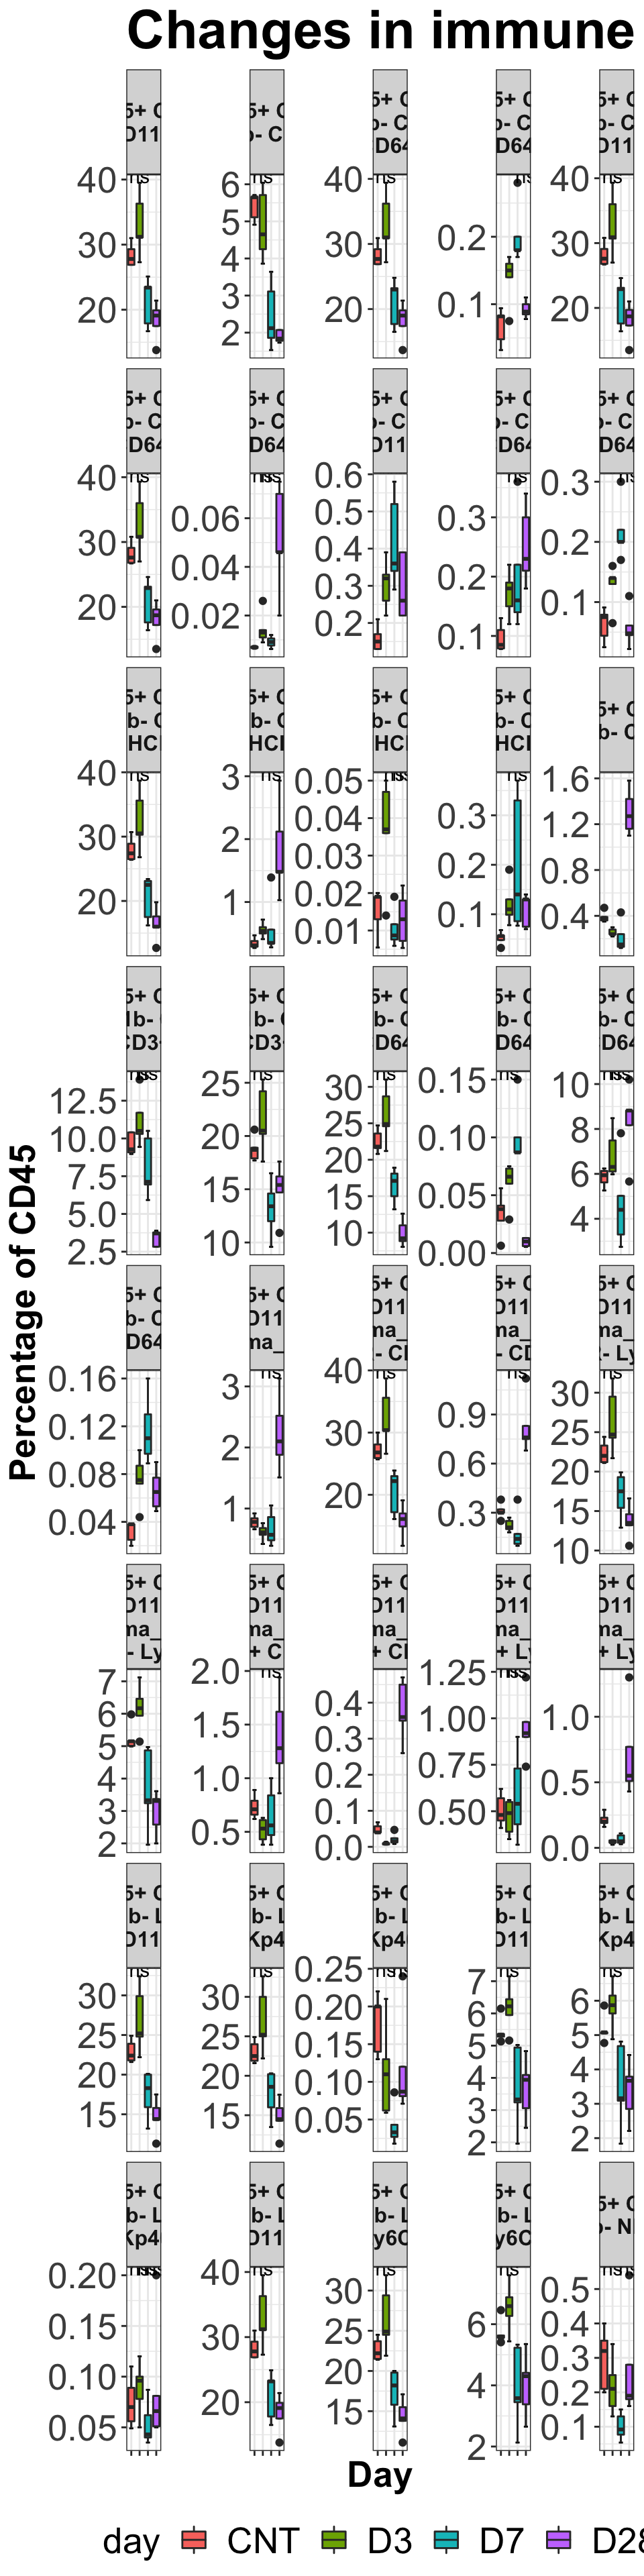
\includegraphics{csu-impactb_files/figure-latex/unnamed-chunk-60-1.pdf}

\begin{Shaded}
\begin{Highlighting}[]
\CommentTok{\# CD3neg\_CD11bpos\_bar\_plot}
\CommentTok{\# CD3neg\_CD11bneg\_bar\_plot}
\end{Highlighting}
\end{Shaded}

\hypertarget{pathology}{%
\chapter{Pathology}\label{pathology}}

\hypertarget{proteomics}{%
\chapter{Proteomics}\label{proteomics}}

For proteomics data, we will be getting data that have already been collected and
pre-processed by another part of the team. The following shows an example of the
type of data we will get as an input:

\begin{Shaded}
\begin{Highlighting}[]
\FunctionTok{library}\NormalTok{(tidyverse)}

\NormalTok{prot\_a }\OtherTok{\textless{}{-}} \FunctionTok{read\_csv}\NormalTok{(}\StringTok{"DATA/Transition Results\_CCTSI\_A.csv"}\NormalTok{)}
\end{Highlighting}
\end{Shaded}

\begin{verbatim}
## Rows: 3393 Columns: 18
## -- Column specification --------------------------------------------------------
## Delimiter: ","
## chr  (7): Peptide, Protein, Replicate, Fragment Ion, Ratio Dot Product, Tota...
## dbl (11): Precursor Mz, Precursor Charge, Product Mz, Product Charge, Retent...
## 
## i Use `spec()` to retrieve the full column specification for this data.
## i Specify the column types or set `show_col_types = FALSE` to quiet this message.
\end{verbatim}

\begin{Shaded}
\begin{Highlighting}[]
\NormalTok{prot\_a}
\end{Highlighting}
\end{Shaded}

\begin{verbatim}
## # A tibble: 3,393 x 18
##    Peptide     Protein Replicate   `Precursor Mz` `Precursor Char~` `Product Mz`
##    <chr>       <chr>   <chr>                <dbl>             <dbl>        <dbl>
##  1 QELDEISTNIR Cfp10   091322_LT1            659.                 2        1061.
##  2 QELDEISTNIR Cfp10   091322_LT2            659.                 2        1061.
##  3 QELDEISTNIR Cfp10   091322_LT3            659.                 2        1061.
##  4 QELDEISTNIR Cfp10   091322_LT4            659.                 2        1061.
##  5 QELDEISTNIR Cfp10   091322_LT5            659.                 2        1061.
##  6 QELDEISTNIR Cfp10   091322_LT6            659.                 2        1061.
##  7 QELDEISTNIR Cfp10   091322_LT7            659.                 2        1061.
##  8 QELDEISTNIR Cfp10   091322_LT8            659.                 2        1061.
##  9 QELDEISTNIR Cfp10   091322_LT10           659.                 2        1061.
## 10 QELDEISTNIR Cfp10   091322_LT11           659.                 2        1061.
## # ... with 3,383 more rows, and 12 more variables: `Product Charge` <dbl>,
## #   `Fragment Ion` <chr>, `Retention Time` <dbl>, Area <dbl>, Background <dbl>,
## #   `Peak Rank` <dbl>, `Ratio Dot Product` <chr>,
## #   `Total Area Normalized` <chr>, `Total Area Ratio` <chr>,
## #   `Library Dot Product` <dbl>, RatioLightToHeavy <dbl>,
## #   DotProductLightToHeavy <dbl>
\end{verbatim}

These data include the following columns:

\begin{itemize}
\tightlist
\item
  \texttt{Peptide}: A short string of peptides that are being measured
\item
  \texttt{Protein}: The protein that those peptides come from
\item
  \texttt{Replicate}: An identifier for the sample that the measurement was taken on
\item
  \texttt{Precursor\ Mz}, \texttt{Precursor\ Charge}, \texttt{Product\ Mz}, \texttt{Product\ Charge},
  \texttt{Fragment\ Ion}, \texttt{Retention\ Time}: Measurements that help in identifying the peptide
  that is being measured (?)
\item
  \texttt{Area}:
\item
  \texttt{Background}:
\item
  \texttt{Peak\ Rank}:
\item
  \texttt{Ratio\ Dot\ Product}:
\item
  \texttt{Total\ Area\ Normalized}:
\item
  \texttt{Total\ Area\ Ratio}
\item
  \texttt{Library\ Dot\ Product}:
\item
  \texttt{RatioLightToHeavy}:
\item
  \texttt{DotProductLightToHeavy}:
\end{itemize}

{[}More about how these data were pre-processed. Softwarei: Skyline{]}

Here are all the unique replicates in this file:

\begin{Shaded}
\begin{Highlighting}[]
\NormalTok{prot\_a }\SpecialCharTok{\%\textgreater{}\%} 
  \FunctionTok{pull}\NormalTok{(Replicate) }\SpecialCharTok{\%\textgreater{}\%} 
  \FunctionTok{unique}\NormalTok{()}
\end{Highlighting}
\end{Shaded}

\begin{verbatim}
##  [1] "091322_LT1"  "091322_LT2"  "091322_LT3"  "091322_LT4"  "091322_LT5" 
##  [6] "091322_LT6"  "091322_LT7"  "091322_LT8"  "091322_LT10" "091322_LT11"
## [11] "091322_LT12" "091322_LT13" "091322_LT14" "091322_H1"   "091322_H2"  
## [16] "091322_H3"   "091322_H4"   "091322_H5"   "091322_H6"   "091322_H7"  
## [21] "091322_H8"   "091322_H9"   "091322_H10"  "091322_H11"  "091322_H12" 
## [26] "091322_H13"  "091322_H14"  "091322_TB1"  "091322_TB2"  "091322_TB3" 
## [31] "091322_TB4"  "091322_TB5"  "091322_TB6"  "091322_TB7"  "091322_TB8" 
## [36] "091322_TB9"  "091322_TB10" "091322_TB11" "091322_TB12"
\end{verbatim}

The three groups in this data are labeled with ``LT'', ``H'', and ``TB'' somewhere in
the identifier. We can create a new column in the dataset that pulls out this
treatment group information:

\begin{Shaded}
\begin{Highlighting}[]
\NormalTok{prot\_a }\OtherTok{\textless{}{-}}\NormalTok{ prot\_a }\SpecialCharTok{\%\textgreater{}\%} 
  \FunctionTok{mutate}\NormalTok{(}\AttributeTok{treatment\_group =} \FunctionTok{str\_extract}\NormalTok{(Replicate, }\StringTok{"[A{-}Z]+"}\NormalTok{)) }

\NormalTok{prot\_a }\SpecialCharTok{\%\textgreater{}\%} 
  \FunctionTok{filter}\NormalTok{(Peptide }\SpecialCharTok{==} \FunctionTok{first}\NormalTok{(Peptide)) }\SpecialCharTok{\%\textgreater{}\%} 
  \FunctionTok{group\_by}\NormalTok{(treatment\_group) }\SpecialCharTok{\%\textgreater{}\%} 
  \FunctionTok{count}\NormalTok{()}
\end{Highlighting}
\end{Shaded}

\begin{verbatim}
## # A tibble: 3 x 2
## # Groups:   treatment_group [3]
##   treatment_group     n
##   <chr>           <int>
## 1 H                 140
## 2 LT                130
## 3 TB                120
\end{verbatim}

\begin{Shaded}
\begin{Highlighting}[]
\NormalTok{prot\_a }\SpecialCharTok{\%\textgreater{}\%} 
  \FunctionTok{filter}\NormalTok{(Peptide }\SpecialCharTok{==} \FunctionTok{first}\NormalTok{(Peptide) }\SpecialCharTok{\&} 
\NormalTok{           Replicate }\SpecialCharTok{==} \FunctionTok{first}\NormalTok{(Replicate))}
\end{Highlighting}
\end{Shaded}

\begin{verbatim}
## # A tibble: 10 x 19
##    Peptide     Protein Replicate  `Precursor Mz` `Precursor Charge` `Product Mz`
##    <chr>       <chr>   <chr>               <dbl>              <dbl>        <dbl>
##  1 QELDEISTNIR Cfp10   091322_LT1           659.                  2        1061.
##  2 QELDEISTNIR Cfp10   091322_LT1           659.                  2         832.
##  3 QELDEISTNIR Cfp10   091322_LT1           659.                  2         703.
##  4 QELDEISTNIR Cfp10   091322_LT1           659.                  2         590.
##  5 QELDEISTNIR Cfp10   091322_LT1           659.                  2         503.
##  6 QELDEISTNIR Cfp10   091322_LT1           664.                  2        1071.
##  7 QELDEISTNIR Cfp10   091322_LT1           664.                  2         842.
##  8 QELDEISTNIR Cfp10   091322_LT1           664.                  2         713.
##  9 QELDEISTNIR Cfp10   091322_LT1           664.                  2         600.
## 10 QELDEISTNIR Cfp10   091322_LT1           664.                  2         513.
## # ... with 13 more variables: `Product Charge` <dbl>, `Fragment Ion` <chr>,
## #   `Retention Time` <dbl>, Area <dbl>, Background <dbl>, `Peak Rank` <dbl>,
## #   `Ratio Dot Product` <chr>, `Total Area Normalized` <chr>,
## #   `Total Area Ratio` <chr>, `Library Dot Product` <dbl>,
## #   RatioLightToHeavy <dbl>, DotProductLightToHeavy <dbl>,
## #   treatment_group <chr>
\end{verbatim}

\begin{Shaded}
\begin{Highlighting}[]
\NormalTok{prot\_a }\SpecialCharTok{\%\textgreater{}\%} 
  \FunctionTok{pull}\NormalTok{(Protein) }\SpecialCharTok{\%\textgreater{}\%} 
  \FunctionTok{unique}\NormalTok{()}
\end{Highlighting}
\end{Shaded}

\begin{verbatim}
## [1] "Cfp10"                  "acpM"                   "Ag85A"                 
## [4] "MtbH37Rv|Rv3841|BfrB"   "MtbH37Rv|Rv1837c|GlcB"  "MtbH37Rv|Rv3418c|GroES"
## [7] "MtbH37Rv|Rv3248c|SahH"  "MtbH37Rv|Rv2031c|hspX"
\end{verbatim}

\begin{itemize}
\tightlist
\item
  Cfp10
\item
  acpM
\item
  Ag85A
\item
  MtbH37Rv\textbar Rv3841\textbar BfrB
\item
  MtbH37Rv\textbar Rv1837c\textbar GlcB
\item
  MtbH37Rv\textbar Rv3418c\textbar GroES
\item
  MtbH37Rv\textbar Rv3248c\textbar SahH
\item
  MtbH37Rv\textbar Rv2031c\textbar hspX
\end{itemize}

  \bibliography{book.bib,packages.bib}

\end{document}
